%-------------------------------------------------------------------------------
% This file provides a skeleton ATLAS note.
% \pdfinclusioncopyfonts=1
% This command may be needed in order to get \ell in PDF plots to appear. Found in
% https://tex.stackexchange.com/questions/322010/pdflatex-glyph-undefined-symbols-disappear-from-included-pdf
%-------------------------------------------------------------------------------
% Specify where ATLAS LaTeX style files can be found.
\newcommand*{\ATLASLATEXPATH}{latex/}
% Use this variant if the files are in a central location, e.g. $HOME/texmf.
% \newcommand*{\ATLASLATEXPATH}{}
%-------------------------------------------------------------------------------
\documentclass[NOTE, atlasdraft=true, texlive=2016, UKenglish]{\ATLASLATEXPATH atlasdoc}
% The language of the document must be set: usually UKenglish or USenglish.
% british and american also work!
% Commonly used options:
%  atlasdraft=true|false This document is an ATLAS draft.
%  texlive=YYYY          Specify TeX Live version (2016 is default).
%  coverpage             Create ATLAS draft cover page for collaboration circulation.
%                        See atlas-draft-cover.tex for a list of variables that should be defined.
%  cernpreprint          Create front page for a CERN preprint.
%                        See atlas-preprint-cover.tex for a list of variables that should be defined.
%  NOTE                  The document is an ATLAS note (draft).
%  PAPER                 The document is an ATLAS paper (draft).
%  CONF                  The document is a CONF note (draft).
%  PUB                   The document is a PUB note (draft).
%  BOOK                  The document is of book form, like an LOI or TDR (draft)
%  txfonts=true|false    Use txfonts rather than the default newtx
%  paper=a4|letter       Set paper size to A4 (default) or letter.

%-------------------------------------------------------------------------------
% Extra packages:
\usepackage{\ATLASLATEXPATH atlaspackage}
% Commonly used options:
%  biblatex=true|false   Use biblatex (default) or bibtex for the bibliography.
%  backend=bibtex        Use the bibtex backend rather than biber.
%  subfigure|subfig|subcaption  to use one of these packages for figures in figures.
%  minimal               Minimal set of packages.
%  default               Standard set of packages.
%  full                  Full set of packages.
%-------------------------------------------------------------------------------
% Style file with biblatex options for ATLAS documents.
\usepackage{\ATLASLATEXPATH atlasbiblatex}

% Package for creating list of authors and contributors to the analysis.
\usepackage{\ATLASLATEXPATH atlascontribute}

% Useful macros
\usepackage{\ATLASLATEXPATH atlasphysics}
\usepackage{xfrac}
\usepackage{enumitem}
\DeclareMathOperator*{\argmax}{argmax}
\DeclareMathOperator*{\argmin}{argmin}
% See doc/atlas_physics.pdf for a list of the defined symbols.
% Default options are:
%   true:  journal, misc, particle, unit, xref
%   false: BSM, heppparticle, hepprocess, hion, jetetmiss, math, process, other, texmf
% See the package for details on the options.

% Files with references for use with biblatex.
% Note that biber gives an error if it finds empty bib files.
\addbibresource{ANA-STDM-2020-17-INT1.bib}
\addbibresource{bib/ATLAS.bib}
\addbibresource{bib/CMS.bib}
\addbibresource{bib/ConfNotes.bib}
\addbibresource{bib/PubNotes.bib}

% Paths for figures - do not forget the / at the end of the directory name.
\graphicspath{{logos/}{figures/}}

% Add you own definitions here (file ANA-STDM-2020-17-INT1-defs.sty).
\usepackage{ANA-STDM-2020-17-INT1-defs}

%-------------------------------------------------------------------------------
% Generic document information
%-------------------------------------------------------------------------------

% Title, abstract and document
%-------------------------------------------------------------------------------
% This file contains the title, author and abstract.
% It also contains all relevant document numbers used for an ATLAS note.
%-------------------------------------------------------------------------------

% Title
\AtlasTitle{A simultaneous measurement of all charged particle properties in $Z$+jets events in $\sqrt{s}=13$ TeV $pp$ collisions using the ATLAS detector}

% Draft version:
% Should be 1.0 for the first circulation, and 2.0 for the second circulation.
% If given, adds draft version on front page, a 'DRAFT' box on top of each other page, 
% and line numbers.
% Comment or remove in final version.
\AtlasVersion{0.2}

%https://atlas-glance.cern.ch/atlas/analysis/analyses/details.php?id=5225

% Abstract - % directly after { is important for correct indentation
\AtlasAbstract{%
This support note describes a measurement of all charged particle properties in $Z$+jets events using the full Run 2 $pp$ collision dataset recorded by the ATLAS detector.  In particular, this is the first analysis to unfold data without binning and using a variable-length and high-dimensional phase space.  The phase space space is defined by the kinematic properties of all charged particles in boosted $Z\to\mu\mu$ events within a fiducial volume. The unfolding is implemented using the recently proposed OmniFold technique, which uses iteratively trained neural networks.  The analysis itself is broken into two part and this note serves as the reference for both parts.  The first part considers the case of a fixed number of observables (MultiFold) while the second part considers the case of all charged particles (OmniFold).
}

% Author - this does not work with revtex (add it after \begin{document})
%\author{The ATLAS Collaboration}

% Authors and list of contributors to the analysis
% \AtlasAuthorContributor also adds the name to the author list
% Include package latex/atlascontribute to use this
% Use authblk package if there are multiple authors, which is included by latex/atlascontribute
 \usepackage{authblk}
% Use the following 3 lines to have all institutes on one line
% \makeatletter
% \renewcommand\AB@affilsepx{, \protect\Affilfont}
% \makeatother
% \renewcommand\Authands{, } % avoid ``. and'' for last author
% \renewcommand\Affilfont{\itshape\small} % affiliation formatting
\AtlasAuthorContributor{Dag Gillberg}{a}{Ntuple production, analysis strategy, MC setup, advising Sandeep and Laura.}
\AtlasAuthorContributor{Sandeep Kaur}{a}{Data stability, jet composition studies, theory systematics.}
\AtlasAuthorContributor{Matt LeBlanc}{b}{Alternative observables.}
\AtlasAuthorContributor{Eric Metodiev}{e}{Short Term Associate.  Initial studies on dataset size.}
\AtlasAuthorContributor{Laura Miller}{a}{Ntuple production, MC setup, analysis strategy, event selection, data-MC comparison, systematics, statisitcal uncertaintiy using boot strapping.}
\AtlasAuthorContributor{Benjamin Nachman}{c}{Unfolding mechanics, event selection cross-check, analysis strategy, advising Adi.}
\AtlasAuthorContributor{Jennifer Roloff}{d}{Track jet studies.}
\AtlasAuthorContributor{Adi Suresh}{c,f}{Unfolding setup, stress-tests, and results.}
% \AtlasAuthorContributor{Second AtlasAuthorContributor}{b}{Author's contribution.}
% \AtlasAuthorContributor{Third AtlasAuthorContributor}{a}{Author's contribution.}
% \AtlasContributor{Fourth AtlasContributor}{Contribution to the analysis.}
% \author[a]{First Author}
% \author[a]{Second Author}
% \author[b]{Third Author}
\affil[c]{Lawrence Berkeley National Laboratory (LBNL)}
\affil[f]{University of California, Berkeley}
\affil[a]{Carleton University}
\affil[b]{European Center for Nuclear Research (CERN)}
\affil[d]{Brookhaven National Laboratory (BNL)}
\affil[e]{Massachusetts Institute of Technology (MIT)}
% \affil[b]{Another Institution}


% If a special author list should be indicated via a link use the following code:
% Include the two lines below if you do not use atlasstyle:
% \usepackage[marginal,hang]{footmisc}
% \setlength{\footnotemargin}{0.5em}
% Use the following lines in all cases:
% \usepackage{authblk}
% \author{The ATLAS Collaboration%
% \thanks{The full author list can be found at:\newline
%   \url{https://atlas.web.cern.ch/Atlas/PUBNOTES/ATL-PHYS-PUB-2016-007/authorlist.pdf}}
% }

% ATLAS reference code, to help ATLAS members to locate the paper
\AtlasRefCode{ANA-STDM-2020-17}

% ATLAS note number. Can be an COM, INT, PUB or CONF note
\AtlasNote{ANA-STDM-2020-17-INT1}

% Author and title for the PDF file
\hypersetup{pdftitle={ATLAS document},pdfauthor={The ATLAS Collaboration}}

%-------------------------------------------------------------------------------
% Content
%-------------------------------------------------------------------------------
\begin{document}

\maketitle

\tableofcontents

% List of contributors - print here or after the Bibliography.
%\PrintAtlasContribute{0.30}
%\clearpage

\clearpage
% Executuive summary + list of contributions, changelog, introduction
\section{Executive summary}
\label{sec:exec}

\subsection{Target}

This analysis uses an innovative machine learning method~\cite{1911.09107} to perform an unbinned, variable- and high-dimensional unfolding using $Z$+jets events. As the first analysis using these new techniques, we limit the phase space to relatively high \pt{} $Z$~bosons in the $Z\to\mu\mu$ channel.   The analysis is broken into two parts, each a significant innovation.  A first round will consider the case of a fixed (but large) number of observables to be simultaneously unfolded (MultiFold).  This first part targets summer/fall 2021.  A second round will consider all charged particles (OmniFold) and targets end of 2021/early 2022.

These data can be used for a variety of studies of Quantum Chromodynamics (QCD), including precision constraints of perturbative QCD, studies of fragmentation, and Monte Carlo event tuning.  New observables that can be constructed with the unfolded phase space can be studied after the measurement and with whatever binning is most natural for the downstream analysis.  This includes complex observables that cannot be unfolded using standard techniques such as the correlation dimension~\cite{Komiske:2019fks} (in the case of OmniFold).

\subsection{Context}

While there is no other measurement that is unbinned, variable- and high-dimensional, there are a variety of related binned measurements of specific observables.   These include track-based observables in inclusive $Z$+jets events at $\sqrt{s}=\SI{8}{\TeV}$~\cite{STDM-2015-14} and various measurements of hadronic final states using tracks~\cite{STDM-2018-57,STDM-2017-33,STDM-2017-16}.  None of these measurements are directly comparable to the one presented in this analysis because of the topology and/or the phase space.  However, as we are using a new methodology for the first time, one of the goals of this paper is to compare the method with standard techniques (e.g.\ Iterative Bayesian Unfolding~\cite{DAGOSTINI1995487,1974AJ.....79..745L,Richardson:72}) in addition to presenting the new unbinned data.

\subsection{Contributors}

\PrintAtlasContribute{0.30}

\clearpage

\section{Changelog}

\begin{itemize}
\item Version 0.1: Initial version, to be used for the editorial board request.
\end{itemize}

\clearpage

\part{Common Components}
\label{part:common}

\textit{All of the sections in this Part are common between the MultiFold and OmniFold analyses.}

%-------------------------------------------------------------------------------
\section{Introduction}
\label{sec:intro}
%-------------------------------------------------------------------------------

The goal of the Large Hadron Collider (LHC) is to infer properties of nature at subnuclear length scales.   One strategy for data analysis is to use models like the Standard Model (SM) and its extensions to fit parameter values to data.  This is an effective strategy that has been used to measure Standard Model couplings and masses as well as to constrain the strength of new physics extensions of the SM.  A key limitation of this parametric approach is that the final result cannot be easily used to infer properties of other parameters or reinterpreted in the context of a different model.  An alternative strategy is to correct data for detector effects in order to measure differential cross sections.  These \textit{unfolded} spectra can be reused for a variety of model interpretations.   Unfolding facilitates data preservation for reuse over time and comparisons across experiments.

The most widely used unfolding methods use various forms of regularized matrix inversion~\cite{DAGOSTINI1995487,Hocker:1995kb,Schmitt:2012kp}.  There are four challenges with these approaches that limit their usefulness.   First, the target observables must be specified prior to unfolding and cannot be changed after the measurement.  Similarly, the binning of the observables must be fixed at the start of the measurement.  Due to the binned nature of existing techniques, most measurements are limited to a small number of observables (usually one) to be simultaneously unfolded.  Finally, the existing methods are not able to account for auxiliary features that determine the resolution of the target observables and thus limit the precision of the measurement.

A variety of alternative unfolding methods have been proposed to solve a subset of these challenges.   For example, some proposals avoid binning~\cite{Glazov:2017vni,Datta:2018mwd,Lindemann:1995ut,Aslan:2003vu} and others use machine learning to improve various aspects of the measurement precision~\cite{Gagunashvili:2010zw,Glazov:2017vni,Datta:2018mwd}.  Recently, three techniques have been proposed that have the potential to address all of the above challenges: OmniFold~\cite{1911.09107}, Conditional GAN Unfolding (CGU)~\cite{Bellagente:2019uyp}, and Conditional Normalizing Flow Unfolding (CNFU)~\cite{Bellagente:2020piv}.   The OmniFold approach scaffolds a simulation with a neural network to perform high- and variable-dimensional reweighting.  The CGU and CNFU methods use neural networks to generate corrected events given detector-level events.

This analysis uses the OmniFold approach to perform the first high- and variable-dimensional unbinned measurement.  In contrast to the CFU and CNFU methods, OmniFold can naturally account for point-cloud nature of collider events (by using e.g. Particle Flow Networks~\cite{Komiske:2018cqr}).  Furthermore, OmniFold reduces to the widely studied Iterative Bayesian Unfolding approach~\cite{DAGOSTINI1995487} when the inputs are binned.  Finally, by using reweighting instead of direct generative modeling, the neural networks need to only learn small corrections to the simulation instead of learning the full probability density of the data.   The physical system chosen for the measurement is the hadronic activity in boosted $Z$ boson events.  Leptonically decaying $Z$ bosons can be identified with high purity and efficiency.  The rest of the event can then be studied with little bias from the event selection.  Charged particles are used due to the precision with which they can be measured.  These events have many tens of charged particles each with a momentum and electric charge and thus the target phase space is about 100-dimensional.

This note is organized as follows.  First, Sec.~\ref{sec:samples} introduces the data and simulated event samples used for the analysis.  Then, Sec.~\ref{sec:objects} describes the objects used in the analysis (in particular, charged particles and tracks).  The analysis methodology is disucssed in Sec.~\ref{sec:strategy} and the prescription for systematic uncertainties appears in Sec.~\ref{sec:uncerts}.  Results are presented in Sec.~\ref{sec:resultsMulti} and Sec.~\ref{sec:resultsOmni} for Multifold and OmniFold respectively, and the note concludes in Sec.~\ref{sec:conclusion}.


%-------------------------------------------------------------------------------
\section{Event samples}
\label{sec:samples}
\input{4_data_MC}

%-------------------------------------------------------------------------------
\section{Event and object selection}
\label{sec:objects}
\subsection{Event selection}
\label{sec:selection}

Initial event selection is outlined in table~\ref{lab:eventsel}. This is primarily designed to remove problematic and background events in favour of the $(Z\to\mu\mu)$+jets signal process. The various cuts are discussed in more detail below.

\begin{table}[h!]
    \centering
    \begin{tabular}{l|l}
         \hline
    \textbf{Event Selection} & \textbf{Description} \\ \hline
    Good Runs List & Event must be part of GRL \\ \hline
    Event Cleaning & No LAr, tile calorimeter, or tracker errors. Event is complete. \\ \hline
    Trigger & Single muon trigger: \\
    & \texttt{HLT\_mu20\_iloose\_L1MU15\_OR\_HLT\_mu50} (2015) \\
    & \texttt{HLT\_mu26\_ivarmedium\_OR\_HLT\_mu50} (2016-18) \\ \hline
    Primary Vertex & $N_{PV}\geq1$ \\ \hline
    Muons & $N_{\text{muons}}\geq2$ \\
          & Opposite charges \\
          & Pass TTVA recommendations for muons \\
          & $81\leq m_{\ell\ell} (\text{GeV})\leq 101$ \\
          & $p_{\text{T},\ell\ell}\geq200$ GeV \\ \hline
    \end{tabular}
    \caption{Overview of the applied event selection.}
    \label{lab:eventsel}
\end{table}

\subsubsection{Event requirements}
The first requirement is that the event must be a part of the ATLAS Good Run Lists (GRL). These are discussed in section~\ref{sec:samples}.

Secondly, the events must pass event cleaning\footnote{The event cleaning procedure is outlined in \url{twiki: https://twiki.cern.ch/twiki/bin/view/Atlas/DataPreparationCheckListForPhysicsAnalysis}}. This removes events that:
\begin{itemize}
    \setlength{\itemsep}{1pt}
    \setlength{\parskip}{0pt}
    \setlength{\parsep}{0pt}
    \item Contain errors in the data collected in the LAr calorimeters (check for error on \texttt{xAOD::EventInfo::LAr})
    \item Contain errors in the data collected in the tile calorimeters (check for error on \texttt{xAOD::EventInfo::Tile})
    \item Contain errors in the silicon tracker data (check for error on \texttt{xAOD::EventInfo::SCT})
    \item Are incomplete due to a restart of the trigger, timing and control system (check for event flag in \texttt{xAOD::EventInfo::Core})
    \item Fail the Loose event cleaning requirement (\texttt{DFCommonJets\_eventClean\_LooseBad}). This is also applied to MC samples.
\end{itemize}

Additionally, it is required that the event in question have at least one primary vertex.

\subsubsection{Trigger requirements}
\label{subsubsec:trigger}
Events are required to pass an unprescaled single muon trigger\footnote{The muon trigger recommendations can be found here: \url{twiki: https://twiki.cern.ch/twiki/bin/view/Atlas/MuonTriggerPhysicsRecommendationsRel212017}}, as outlined in table~\ref{lab:eventsel}.
The recommended trigger is dependent on the year in which the data was taken (or the year of the corresponding Monte Carlo sample).

\subsubsection{Dimuon system requirements}
\label{subsubsec:TTVA_selection}
The event is required to have at least two muons of opposite charge, with a dilepton mass between 81 GeV and 101 GeV in order to ensure the muons originate from a $Z$ boson.

Additionally, the muons must pass track-to-vertex association recommendations\footnote{Recommendations are given by the tracking group and are outlined here: \url{twiki: https://twiki.cern.ch/twiki/bin/view/AtlasProtected/TrackingCPEOYE2015}} as follows:

\begin{itemize}
    \item $|d_0^{BL}\text{significance}| < $ 3
    \item $|\Delta z_0^{BL}\sin\theta| < 0.5 $mm
\end{itemize}

where $d_0$ and $z_0$ represent the point along the track with the closest approach to the beamspot.

The large $p_{\text{T},\ell\ell}$ cut of 200~GeV has been chosen to ensure that the balancing jet(s) have a high quantity of charged particles, as these are the primary subject of the analysis.
Events with a $p_{\text{T},\ell\ell}$ larger than 165~GeV are saved in order to study migration effects between truth and reconstructed events (i.e. events where the reconstructed $p_{\text{T},\ell\ell}$
is smaller than 200 GeV, but is larger than 200 GeV at truth level and vice versa).

\subsection{Detector-level objects}

\paragraph{Muons} are reconstructed using a combination of information from the muon spectrometer (MS) and the inner detector (ID). Occasionally, the ATLAS calorimeters are used to provide additional information for reconstruction. The reconstruction process is described in detail in reference~\cite{Aad:2016jkr}.
The muons are required to pass Medium quality selection using the \texttt{MuonSelectionTool}\footnote{The twiki detailing the MuonSelectionTool: \url{twiki: https://twiki.cern.ch/twiki/bin/view/Atlas/MuonSelectionToolR21}} and the \texttt{PflowLoose\_VarRad} isolation working point as given by
the \texttt{IsolationTool}\footnote{Information on the isolations WPs and the tool: \url{twiki: https://twiki.cern.ch/twiki/bin/view/AtlasProtected/RecommendedIsolationWPs}}. The simulated muons are also calibrated in order to correct for $p_\text{T}$ discrepancies between data and simulation~\cite{Aad:2016jkr}.
Kinematically, muons are required to have a minimum $\pt$ of 25~GeV, and have $|\eta|<2.4$.

\paragraph{Tracks} are reconstructed from charged-particle hits within the silicon- and straw-tube based inner tracking detectors. They are required to pass the Loose quality working point and to be associated with the primary vertex of the event using the Tight track-to-vertex association\footnote{Information on both the selection tool and the TTVA tool may be found here: \url{twiki: https://twiki.cern.ch/twiki/bin/view/AtlasProtected/TrackingCPRecsRun2Final}}.
The primary vertex is defined as the reconstructed vertex with the highest sum of associated track $\pt^2$. Tracks are required to have a $\pt>500$~\MeV~to be included in this measurement.  The track $\eta$ and $\phi$ coordinates come from the five-parameter track fit to $(\eta,\phi,q/p,d_0,z_0)$, and thus correspond to the track coordinates at the origin.
In addition, tracks which are associated with the muons are not considered part of the final track collection.

\paragraph{Jets} are reconstructed using the anti-$k_t$ algorithm~\cite{Cacciari:2008gp} with a radius parameter of $R=0.4$. Particle flow objects~\cite{Aaboud:2017aca} are used as input. The jets are calibrated using the recommended procedure for small-$R$ jets, this includes: MCJES calibration, global sequential calibration, and in-situ calibration.
Jets are required to have a calibrated $p_\text{T} > 10~\text{GeV}$ and rapidity $|y| < 4.4$\footnote{General recommendations are found here: \url{twiki: https://twiki.cern.ch/twiki/bin/view/AtlasProtected/JetEtmissRecommendationsR21}}. Note that while these are saved as objects during the analysis, they are not currently being used.

\paragraph{Track Jets} are also reconstructed using the anti-$k_t$ algorithm with a radius parameter of $R=0.4$. All tracks which pass the selection described above are used as input, and clustering is completed using \textsc{FastJet}~\cite{Cacciari:2011ma}.

\subsubsection{Overlap Removal}

There is a possibility that an electron may be misidentified as a jet during reconstruction, so in cases where the jet is found to be within $\Delta R < 0.2$ of a reconstructed electron, the jet is removed.
Additionally, a specialized overlap removal procedure must be applied between muons and jets due to a bug in the particle flow algorithm which results in sub-leading muon tracks being included in the particle flow objects~\footnote{A brief summary of the bug and the overlap removal procedure can be found here: \url{https://indico.cern.ch/event/807799/contributions/3362328/attachments/1818680/2973610/Presentation.pdf},
and here: \url{https://indico.cern.ch/event/814156/contributions/3396841/attachments/1830226/2997072/Presentation.pdf}}.
The muon is preferentially kept in this case, so it does not limit our analysis as the jets are not currently used.

A summary of the detector level event selection can be found in table~\ref{tab:ObjCuts}.


\begin{table}[h!]
    \centering
    \begin{tabular}{l|l}
    \hline
     \textbf{Object} & \textbf{Additional Selection Criteria} \\ \hline
     Muons & $\pt>25~\GeV$, $|\eta|<2.4$ \\
           & Medium quality, pass isolation \texttt{PflowLoose\_VarRad} \\ \hline
     Jets (\texttt{AntiKt4EMPFlowJets}) & $\pt>10~\GeV$, $|y|<4.4$ \\
                                        & $\Delta R_{e,jet} > 0.2$ \\
                                        & Muon-PFlow jet overlap removal \\ \hline
     Tracks & $p_{\text{T}} > 500$ MeV \\
            & Loose Quality \\
            & Tight TTVA \\
            & Do not originate from a muon \\ \hline
     Track Jets & Input tracks must pass the above cuts \\ \hline
    \end{tabular}
    \caption{Object level cuts}
    \label{tab:ObjCuts}
\end{table}

\subsection{Particle-level objects}

Stable charged particles ($c\tau$ > 10 mm) are used to define the analog of tracks at particle-level. Charged-particles are required to have $\pt > 500$~\MeV~and $|\eta|<2.5$.
Muons are dressed using all photons within a radius of $R=0.1$ and identical kinematic cuts are applied to those used at the detector-level.
\texttt{TruthWZJets} are utilized at the particle-level, which are constructed utilizing the anti-$k_t$ algorithm with $R=0.4$ from all particle 4-vectors except for prompt leptons from $W$, $Z$, Higgs, and $\tau$ decay, and photons within a cone of $R=0.1$ around the prompt lepton.
Track jets at the particle-level are constructed using the same process as at the detector-level, but the charged particles are used as input.
Objects at particle-level, as well as the truth phase space, are summarized in table~\ref{tab:PLObjCuts}.

\begin{table}[h!]
    \centering
    \begin{tabular}{l|l}
    \hline
    \textbf{Object} & \textbf{Acceptance} \\ \hline
    Dressed Muons & $p_\text{T} > 25$ GeV, $|\eta| < 2.4$ \\\hline
    Jets (\texttt{TruthWZJets}) & $p_\text{T} > 10$ GeV, $|y|<4.4$ \\\hline
    Charged Hadrons & $p_\text{T}>500$ MeV, $|\eta|<2.5$  \\ \hline
    Track Jets & Charged hadrons used as input must pass above criteria \\ \hline
    Phase Space & At least two oppositely charged muons \\
    & $81<m_{\ell\ell}~\GeV<101$ \\
    & $p_{\text{T},\ell\ell}>200$ GeV \\ \hline
    \end{tabular}
    \caption{Fiducial object cuts and the truth phase space}
    \label{tab:PLObjCuts}
\end{table}

\subsection{Corrections to Monte Carlo samples}
\label{subsec:MCCorr}
\subsubsection{Pileup reweighting}
\label{subsec:PRW}
When events in MC samples are produced, the interactions per bunch crossing, $\mu$, is assigned a certain value. This can differ from the values that are actually seen in the corresponding data, thus it is
necessary to correct the MC events such that the distribution of $\mu$ is equivalent to what is observed in data.

The \texttt{PileupReweightingTool}\footnote{Details can be found here: \url{twiki: https://twiki.cern.ch/twiki/bin/view/AtlasProtected/ExtendedPileupReweighting}} uses the $\mu$ and the run number assigned to the MC event along with the luminosity of the corresponding data in the same run number to determine the pileup weight to be applied to the event.
This requires that both the $\mu$ distribution for the specific MC sample is available to the tool, as well as the files used to calculate the luminosity for the data. As we use unprescaled triggers in this analysis, the centrally produced lumicalc files corresponding to the GoodRunsLists in section~\ref{subsec:data} are used.
Configuration files for the tool for each MC sample are also provided centrally.
The pileup weight is then multiplied with the MC event weight in order to correct the $\mu$.

The tool also provides a scaling correction for data. The MC simulation for a given $\mu$ value is known to be too hard, therefore the $\mu$ values in data are scaled down to account for this.

\subsubsection{Trigger scale factor}
There are differing trigger efficiencies between data and MC simulation, thus a correction in the form of a scale factor applied to the event weight is necessary for MC events. The triggers used in this analysis are outlined in section~\ref{subsubsec:trigger}.

\subsubsection{Muon scale factors}
Muon scale factors related to reconstruction efficiency, isolation efficiency, and track-to-vertex (TTVA) efficiency are derived from $J/\psi$ and $Z$ events using the tag-and-probe method for muons in the central region. The resulting scale factors are applied to the event weight in the same way as the trigger scale
factor\footnote{Addtional information on both the trigger and muon scale factors may be found in the muon analysis twiki: \url{twiki: https://twiki.cern.ch/twiki/bin/view/AtlasProtected/MCPAnalysisGuidelinesMC16}}.


\newpage

\subsection{Observed and predicted event yields}
\label{sec:cutflow}

Table~\ref{tab:CFComp} presents the predicted and observed event yields after applying the analysis cuts consecutively to data and the 2 MC samples for each year, and table~\ref{tab:RelCF} shows the associated relative efficiency.  Note that the event selection has been validated using an independent implementation of the analysis event selection using the $ZH\rightarrow aa\rightarrow gggg$ analysis framework\footnote{We thank Murtaza Safdari for helping with this.  The analysis code is built on the BHamAnalyaisFramework: \url{https://gitlab.cern.ch/atlas-physics/HDBS/HBSM/higgs_axion_axion/-/tree/workingCompile/BhamAnalysisFramework}.}.

\begin{table}[h!]
    \centering
    \begin{tabular}{l|l|l|l|l|l|l}
    \hline\hline
    \textbf{Sample} & \multicolumn{6}{c}{\textbf{Cuts}} \\ \hline
     & None & DQ & Trigger & Dilepton & $p_{\text{T},\ell\ell}$ & $p_{\text{T},\ell\ell}$ \\
     &  &  &  &  & $>165~\GeV$ & $>200~\GeV$ \\ \hline\hline
    Data 2015--2016 & 475.7M & 462.5M & 72.89M & 20.27M & 103.5k & 54.92k \\ \hline
    Powheg Pythia 8 MC16a & 70.63M & 70.28M & 41.76M & 20.13M & 79.34k & 41.17k \\ \hline
    Sherpa 2.2.1 MC16a & 75.60M & 75.21M & 42.84M & 20.07M & 96.75k & 52.05k \\ \hline\hline
    Data 2017 & 282.8M & 270.5M & 84.38M & 24.15M & 124.2k & 65.87k \\ \hline
    Powheg Pythia 8 MC16d & 86.42M & 85.88M & 50.35M & 24.45M & 96.58k & 50.08k \\ \hline
    Sherpa 2.2.1 MC16d & 92.50M & 91.90M & 51.59M & 24.41M & 118.3k & 63.30k \\ \hline\hline
    Data 2018 & 357.0M & 348.7M & 116.8M & 35.99M & 163.4k & 86.35k \\ \hline
    Powheg Pythia 8 MC16e & 114.0M & 113.3M & 67.22M & 32.46M & 128.2k & 66.56k \\ \hline
    Sherpa 2.2.1 MC16e & 122.0M & 121.3M & 68.93M & 36.41M & 155.9k & 83.23k \\ \hline\hline
    \end{tabular}
    \caption{Number of events remaining after each cut applied during the analysis. Data Quality (DQ) includes the GRL and event cleaning criteria.
    Dilepton includes the requirement of 2 oppositely charged muons which pass TTVA and trigger matching requirements, as well as the $m_{\ell\ell}$ cut.
    Differences between MC and data are expected up to the dilepton cut as data contains QCD background while the MC samples do not.}
    \label{tab:CFComp}
\end{table}

\begin{table}[h!]
  \centering
  \begin{tabular}{l|l|l|l|l|l}
  \hline\hline
  \textbf{Sample} & \multicolumn{5}{c}{\textbf{Cuts}} \\ \hline
    & DQ & Trigger & Dilepton & $p_{\text{T},\ell\ell}$ & $p_{\text{T},\ell\ell}$ \\
    &  &  &  & $>165~\GeV$ & $>200~\GeV$ \\ \hline\hline
   Data 2015--2016 & -2.46\% & -84.24\% & -72.20\% & -99.49\% & -46.93\% \\ \hline
   Powheg Pythia 8 MC16a & -0.50\% & -40.58\% & -51.80\% & -99.61\% & -48.11\% \\ \hline
   Sherpa 2.2.1 MC16a & -0.50\% & -43.04\% & -53.15\% & -99.52\% & -46.21\% \\ \hline\hline
   Data 2017 & -4.35\% & -68.61\% & -71.38\% & -99.49\% & -46.93\% \\ \hline
   Powheg Pythia 8 MC16d & -0.63\% & -41.37\% & -51.45\% & -99.60\% & -48.15\% \\ \hline
   Sherpa 2.2.1 MC16d & -0.64\% & -43.87\% & -52.68\% & -99.52\% & -46.51\% \\ \hline\hline
   Data 2018 & -2.30\% & -66.50\% & -72.88\% & -99.48\% & -47.04\% \\ \hline
   Powheg Pythia 8 MC16e & -0.60\% & -40.69\% & -51.70\% & -99.61\% & -48.97\% \\ \hline
   Sherpa 2.2.1 MC16e & -0.60\% & -43.17\% & -52.95\% & -99.52\% & -46.63\% \\ \hline\hline
   \end{tabular}
   \caption{The relative number of events rejected after each cut relative to the previous cut}
   \label{tab:RelCF}
\end{table}

\subsection{Data stability tests}
\label{sec:data-stability}
To check stability of data used for this analysis, rate for each year is calculated by dividing event counts from a set of runs by their associated total integrated luminosity. Events are counted if they pass the event selection with $p_{\text{T},\ell\ell}>165$ GeV. Consecutive runs are combined until the integrated luminosity amount to at least 2 fb$^{-1}$. Figure~\ref{fig:DataStability} depicts the rate for year 2015 to 2018, where each time-ordered data bin contains data 2 fb$^{-1}$ luminosity. The first bin shows rate for year 2015, bins 2--16 are for year 2016, bins 17--37 and 38--64 represent rate for year 2017 and 2018 respectively. Further, to consider those residual runs having combined luminosities smaller than 2 fb$^{-1}$, the last bin for each year is merged with the previous bin. The calculated average rate for year 2015--2018 is 2812 $\pm$ 4 and shows reasonable consistency for each year. Figure~\ref{fig:DataStability} shows the stability of data for each year used in this analysis.
\begin{figure}[h!]
  \centering
  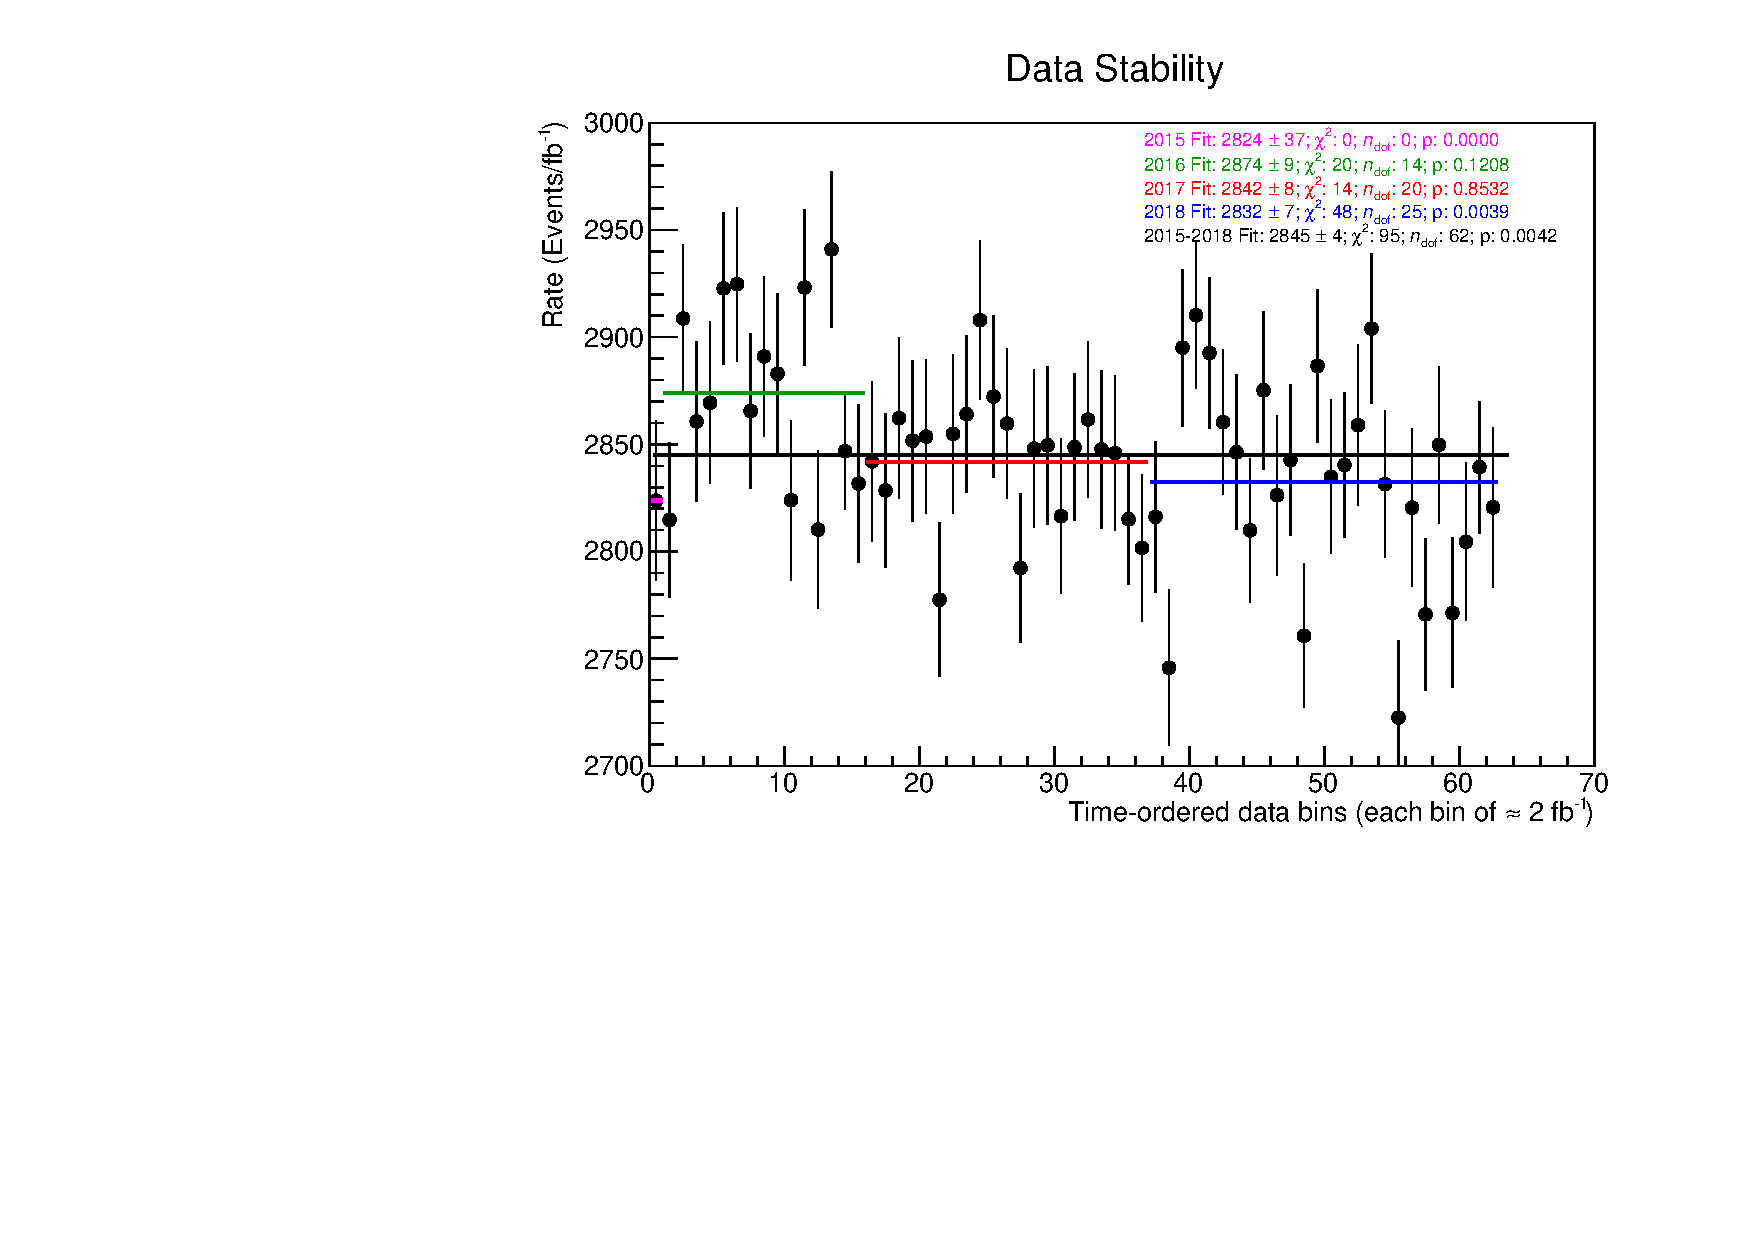
\includegraphics[width=0.75\textwidth]{figures/DataStability.pdf}
  \caption{Events per fb$^{-1}$ for year 2015 to 2018, where each time-ordered data bin contains 2 fb$^{-1}$ luminosity.
    $p$-values and chi-squared values are calculated using statistical uncertainty only. Additional bias is expected due to the changing beam conditions (more or less pileup, affecting e.g.\ lepton isolation).
  }
  \label{fig:DataStability}
\end{figure}

\subsection{Observed and predicted kinematic distributions}
\label{sec:datamc}
Figure~\ref{fig:MuActual} shows the actual interactions per bunch crossing $\mu$ for the individual data periods, as well as the full Run 2 dataset.
Figure~\ref{fig:pTmll} gives the $\pt$ and $m$ distributions for the dilepton system, and figure~\ref{fig:pTetamus} gives the $\pt$ and $\eta$ distributions for both the leading and sub-leading muon.
The $\pt$ and $y$ distributions for the leading and sub-leading track jet are shown in figure~\ref{fig:pTyjets}, and figure~\ref{fig:jetsubstructure} and~\ref{fig:ntrackinjets} show some
selected jet substructure variables and the number of constituents, respectively.  The substructure variables are the $n$-subjettiness observables~\cite{Thaler:2010tr,Thaler:2011gf}, which have the form

\begin{align}
\tau_N=\left(\frac{1}{\sum_{i\in\text{jet}} R_0p_{T,i}}\right)\sum_{i\in\text{jet}} p_{T,i}\min_{j\in\{1,...,N\}}\left\{\Delta R_{j,n}\right\}\,,
\end{align}
%
where $R_0$ is the jet algorithm radius and $\Delta R_{j,n}$ is the $\Delta R$ between the jet constituent and the $j^\text{th}$ subjet axis. Finally, the properties of the tracks used for the analysis are shown in figure~\ref{fig:trackInfo}.

Additional figures with these distributions shown per year of data taking can be found in appendix~\ref{app:AddDataMC}.

\begin{figure}[h!]
  \centering
  \includegraphics[page=5,width=0.45\textwidth]{figures/ZjetOmnifoldMCDataComp.pdf}
  \includegraphics[page=6,width=0.45\textwidth]{figures/ZjetOmnifoldMCDataComp.pdf} \\
  \includegraphics[page=7,width=0.45\textwidth]{figures/ZjetOmnifoldMCDataComp.pdf}
  \includegraphics[page=8,width=0.45\textwidth]{figures/ZjetOmnifoldMCDataComp.pdf}
  \caption{The ``actual'' mean interactions per bunch crossing, $\mu$, for 2015--2016 data (top left), 2017 data (top right), 2018 data (bottom left), and the full Run-2 dataset (bottom right). Note that the pileup-reweighing uses actual $\mu$ for 2017 and 2018 data, while $\mu_\mathrm{avg}$, i.e.\ $\mu$ calculated by averaging the actual $\mu$ of all bunches, were used for 2015--2016 data. Hence a worse agreement is seen for this period.}
  \label{fig:MuActual}
\end{figure}

\begin{figure}[h!]
  \centering
  \includegraphics[page=12,width=0.45\textwidth]{figures/ZjetOmnifoldMCDataComp.pdf}
  \includegraphics[page=16,width=0.45\textwidth]{figures/ZjetOmnifoldMCDataComp.pdf}
  \caption{Distributions for the $\pt$ and $m$ of the dilepton system. Due to the high $\pt$ phase space, it is expected that the MC simulation will underpredict the data.}
  \label{fig:pTmll}
\end{figure}

\begin{figure}[h!]
  \centering
  \subfloat[Leading muon]{\includegraphics[page=24,width=0.45\textwidth]{figures/ZjetOmnifoldMCDataComp.pdf}\includegraphics[page=32,width=0.45\textwidth]{figures/ZjetOmnifoldMCDataComp.pdf}} \\
  \subfloat[Sub-leading muon]{\includegraphics[page=28,width=0.45\textwidth]{figures/ZjetOmnifoldMCDataComp.pdf}\includegraphics[page=36,width=0.45\textwidth]{figures/ZjetOmnifoldMCDataComp.pdf}}
  \caption{The $\pt$ and $\eta$ distributions for the (a) leading and (b) the sub-leading muon}
  \label{fig:pTetamus}
\end{figure}

\begin{figure}[h!]
  \centering
  \subfloat[Leading track jet]{\includegraphics[page=72,width=0.45\textwidth]{figures/ZjetOmnifoldMCDataComp.pdf}\includegraphics[page=76,width=0.45\textwidth]{figures/ZjetOmnifoldMCDataComp.pdf}} \\
  \subfloat[Sub-leading track jet]{\includegraphics[page=88,width=0.45\textwidth]{figures/ZjetOmnifoldMCDataComp.pdf}\includegraphics[page=92,width=0.45\textwidth]{figures/ZjetOmnifoldMCDataComp.pdf}}
  \caption{The $\pt$ and $y$ distributions for the (a) leading and (b) the sub-leading jet}
  \label{fig:pTyjets}
\end{figure}

\begin{figure}[h!]
  \centering
  \includegraphics[page=84,width=0.45\textwidth]{figures/ZjetOmnifoldMCDataComp.pdf}
  \includegraphics[page=100,width=0.45\textwidth]{figures/ZjetOmnifoldMCDataComp.pdf} \\
  \includegraphics[page=104,width=0.45\textwidth]{figures/ZjetOmnifoldMCDataComp.pdf}
    \includegraphics[page=116,width=0.45\textwidth]{figures/ZjetOmnifoldMCDataComp.pdf}\\
  \includegraphics[page=108,width=0.45\textwidth]{figures/ZjetOmnifoldMCDataComp.pdf}
      \includegraphics[page=120,width=0.45\textwidth]{figures/ZjetOmnifoldMCDataComp.pdf}\\
  \includegraphics[page=112,width=0.45\textwidth]{figures/ZjetOmnifoldMCDataComp.pdf}
      \includegraphics[page=124,width=0.45\textwidth]{figures/ZjetOmnifoldMCDataComp.pdf}
  \caption{Jet substructure features for the leading (left) and subleading (right) track jets.}
  \label{fig:jetsubstructure}
\end{figure}

\begin{figure}[h!]
  \centering
  \includegraphics[page=136,width=0.45\textwidth]{figures/ZjetOmnifoldMCDataComp.pdf}
  \includegraphics[page=140,width=0.45\textwidth]{figures/ZjetOmnifoldMCDataComp.pdf} \\
  \caption{The number of constituents in the leading (left) and subleading (right) track jets.}
  \label{fig:ntrackinjets}
\end{figure}

\begin{figure}[h!]
  \centering
  \includegraphics[page=128,width=0.45\textwidth]{figures/ZjetOmnifoldMCDataComp.pdf}
  \includegraphics[page=144,width=0.45\textwidth]{figures/ZjetOmnifoldMCDataComp.pdf} \\
  \includegraphics[page=148,width=0.45\textwidth]{figures/ZjetOmnifoldMCDataComp.pdf}
  \includegraphics[page=152,width=0.45\textwidth]{figures/ZjetOmnifoldMCDataComp.pdf}
  \caption{Distributions for the number of tracks per event (top left), and the $\pt$ (top right), $\eta$ (bottom left), and $\phi$ (bottom right) for each reconstructed track}
  \label{fig:trackInfo}
\end{figure}

\clearpage
\subsection{Event displays}
\label{sec:event-displays}

Figure~\ref{fig:EventDisplay} shows an event display for an event that passes the event selection. This event contains two muons and 45 charged hadrons at the truth level (with $\pt>\SI{0.5}{\GeV}$ and $|\eta|<2.5$). 37 tracks are reconstructed. Most tracks have a clear matching truth particles, but we can see many examples of charged hadrons that did not produce a track, and some examples of ``fake'' tracks that do not have any matching charged truth hadron. More event displays like this are listed in Appendix~\ref{app:event-displays}.

\begin{figure}[h!]
  \centering
  \includegraphics[page=26,width=0.48\textwidth]{figures/EventDisplays.pdf}
  \includegraphics[page=27,width=0.48\textwidth]{figures/EventDisplays.pdf} \\
  \includegraphics[page=29,width=0.48\textwidth]{figures/EventDisplays.pdf}
  \includegraphics[page=30,width=0.48\textwidth]{figures/EventDisplays.pdf}
  \caption{Displays of a simulated event that passes all cuts. Full event views are provided both at the reconstructed level (top left) and at the particle level (top right).
    Muons are shown as red dots, the charged particles (hadrons or tracks) are shown as gray or black crosses and the dilepton system is displayed as a red cross.
    Track jets are shown as blue circles, and leading jet constituents are represented with black crosses.
    A zoomed view of the leading jet is shown at the bottom left simultaneously for reconstructed tracks and truth charged hadrons. The momenta for most particles in the event are also listed (bottom right).
    Note that the goal with the OmniFold analysis is to provide unfolded events that contain a list of four vectors corresponding to all individual particles seen in the upper right figure: two muons, and a full list of charged hadrons particles.}
  \label{fig:EventDisplay}
\end{figure}

\clearpage


%-------------------------------------------------------------------------------
\section{Methodology}
\label{sec:strategy}

\subsection{Unfolding procedures}

\subsubsection{Introduction}
\label{sec:UnfoldIntro}

Unfolding is the process of removing detector effects from data in order to infer the properties of particle-level spectra (see~\cite{Cowan:2002in,Blobel:2203257,doi:10.1002/9783527653416.ch6,Balasubramanian:2019itp} for reviews).  In other fields, this is often called \textit{deconvolution}, since one can think of detector effects as the convolution of a noise function with the spectrum of interest.  Unfolding needs to correct for many effects:

\begin{enumerate}[label={(\arabic*)}]
\item Acceptance and efficiency: particles produced may not be measured.
\item Detector noise: particles measured may not be from real particles, at least not the desired particles (e.g. fakes) within a fiducial volume (migrating into acceptance).
\item Background processes: if one wants to measure the differential cross section of a particular process, then you may want to subtract the contributions from background processes.
\item Combinatorics: if there are $n$ particles and you want to measure the properties of a particular order (e.g. leading $p_T$), the detector effects can change the order.
\item Detector distortions: the detector response introduces bias and resolution effects.
\end{enumerate}

A well-structured measurement will be dominated by (5).  It is possible to setup a measurement so that (4) is not relevant (e.g. operating at the level of events as sets instead of using individual objects).  By using a pure (e.g. $Z$+jets) or inclusive (e.g. dijets) event selection, (3) can be made irrelevant.  It is also possible to mitigate (1) and (2) by performing the unfolding in a bigger phase space than is eventually used for the final measurement.  In our case, we will also reduce these effects by using the highly efficient $Z$ to select events and then using (mostly) the hadronic recoil for the measurement.

Corrections are derived using simulations, by creating a match between particle-level events and detector-level events.  Until now, all measurements in high energy physics have been performed using binned data.   In this case, detector effects can be modeled by a set of linear equations:
\begin{align}
\label{eq:foldingequation}
\left(\textbf{R}\cdot (\textbf{t}\odot \textbf{c})\right)\odot 1/\textbf{f}+\textbf{b}=\textbf{d}\,,
\end{align}
where bold letters denote vectors or matrices, $\cdot$ is the usual matrix product, $\odot$ is the Hadamard (component-wise) product, and the division is defined component-wise\footnote{An equivalent way to write Eq.~\ref{eq:foldingequation} is $\left(\sum_{i}R_{ij}\,t_i\,c_i\right)/f_j+b_j=d_j$, where $i$ and $j$ are indices for the reconstructed and particle level bins, respectively.}. The symbol $\textbf{t}$ is the particle-level distribution, $\textbf{d}$ is the detector-level distribution, $\textbf{b}$ is the background detector-level distribution, and $\textbf{R}$ is the response matrix.  The correction factors $\textbf{c}$ represent the fraction of particle-level events that also pass the detector-level selection and the fake factors $\textbf{f}$ represent the fraction of detector-level events that have a corresponding particle-level event that passes the selection.  The solution to Eq.~\ref{eq:foldingequation} is given by
\begin{align}
\label{eq:unfolding}
\textbf{t}_\text{measured} = \textbf{R}^{-1}\left( (\textbf{d}-\textbf{b})\odot \textbf{f}\right)\odot 1/\textbf{c}.
\end{align}
Many of the of the common unfolding methods follow the form in Eq.~\ref{eq:unfolding}.
Uncertainties on the measurement are obtained using uncertainty propagation. In particular, the unfolding uncertainties are evaluated by varying the response matrix term $\mathbf{R}^{-1}$, which typically is done coherently with the $\mathbf{f}$ and $\mathbf{c}$ terms (e.g.\ by switching MC generator or propagating an experimental or theoretical systematic that affect the event kinematics).
%but vary in their estimation of $\textbf{R}^{-1}$.
For a variety of reasons, it is advantageous to not directly invert the response matrix.  In particular, \textbf{R} may not be invertible because it is singular or not even a square matrix.  The simple matrix inverse is also susceptible to oscillations from significant off-diagonal components.

One of the most widely used unfolding methods is the Iterative Bayesian Unfolding (IBU) technique\footnote{In other fields, this is called Lucy-Richardson deconvolution~\cite{1974AJ.....79..745L,Richardson:72}.}.   For simplicity, assume that $\textbf{b}=\textbf{0}$ and $\textbf{f}=\textbf{c}=\textbf{1}$.  When this is not the case, these are corrected for in the binned case as done in Eq.~\ref{eq:unfolding}.   The IBU method then proceeds as follows:
\begin{align}
t_i^{(n)}&=\sum_j \Pr(t_i|d_j) d_j \\
&=\sum_j \frac{\Pr(d_j|t_i)\Pr^{(n)}(t_i)}{\sum_i \Pr(d_j|t_i)\Pr^{(n)}(t_i)} d_j \\
&=\sum_j \frac{R_{ji}\Pr^{(n)}(t_i)}{\sum_i R_{ji}\Pr^{(n)}(t_i)} d_j.
\end{align}
%
Typically, one choses the prior $\Pr^{(n)}(t_i)=t_i^{(n-1)}$ and $\Pr^{(0)}(t_i)=t_i$ (from simulation), assuming $\textbf{t}$ is normalized.  It has been shown that as $n\rightarrow\infty$, the IBU estimate approaches the maximum likelihood estimator~\cite{shepp1982maximum}.  Typically, $n\sim 3$ as a form of regularization to balance amplifying statistical fluctuations with mitigating systematic uncertainties from the prior dependence.

\subsubsection{OmniFold}
\label{subsec:omnifold}

IBU and other standard unfolding methods face three challenges.  First, they require the data to be binned.  This binning must be chosen ahead of time and is often chosen manually.  Second, only a small number of observables (or a small number of bins for a given number of observables) can be unfolded simultaneously in order to keep the total number of bins to a manageable level.  Finally, the matrix $\textbf{R}$ only depends on the unfolded features and not on any other auxiliary features that may be useful for determining the detector response.  Even though the inputs to the unfolding may be calibrated, if the detector response depends on additional features, the result will be suboptimal and potentially biased.

OmniFold is an approach that addresses all three of the above challenges by using neural networks.  Like IBU, OmniFold is an iterative method.  Furthermore, OmniFold is a natural generalization of IBU in the sense that when the OmniFold method is applied to binned data, it reproduces IBU at each iteration.
As the Omnifold method is unbinned, it works directly with events and we will use $\vec{x}_i$ as the particle-level properties of event $i$, and $\vec{x}_{\mathrm{reco},i}$ would be the corresponding detector-level quantities ($i$ is no longer a bin index as in previous equations).  The properties could be a fixed set of observables or they could be a variable-length set of particles, each with their own properties.  OmniFold can handle any of these cases (with a suitably chosen neural network architecture).
The OmniFold method proceeds as follows:

\begin{description}
\item Iterate:
  \begin{enumerate}[label={(\arabic*)}]
    \item Determine a reweighting function $\omega(\vec{x}_\mathrm{reco})$ that adjusts the detector-level simulation ('MC Reco') to match data ('Data Reco').
    \item Propagate the weights from (1) to the particle-level simulation ('MC Truth'), and determine a new reweighting function $\nu(\vec{x})$ that replicates this reweighing based on particle-level quantities $\vec{x}$. The particle level weights $\nu(\vec{x})$ are next propagated to detector-level.
 \end{enumerate}
\end{description}
%
The final result after $n$ iterations is a function $\nu(\vec{x})$ that provides weights to a particle-level MC sample such that will become ``unfolded data'' for any observable constructed from the event features $\vec{x}$.

As an algorithm, the OmniFold procedure does not require neural networks; however, these tools are well-suited to be the reweighting functions described above (more on this below).  Step (2) of the OmniFold algorithm is important because the weights from (1) are not a function of the particle-level phase space.  In particular, two events in the same particle-level phase space can be mapped to different detector-level events.  However, to be a proper unfolding, we require that two events with the same particle-level phase space have the same weight.  This is achieved with Step (2).

The OmniFold procedure is illustrated schematically in Fig.~\ref{fig:omnifoldschematic}.  The detector-level weights at a given step are represented by the symbol $\omega_n$ while the particle-level weights are represented by the symbol $\nu_n$.  Note that for Step (2), we could reweight from the original particle-level simulation to the weighted simulation or from the weights derived at the previous step to weights from (1).  Both achieve the same results, but there may be advantages to learning an incremental reweighting (as in Fig.~\ref{fig:omnifoldschematic}) since each step is a correction on the previous step.

As mentioned, the output of the OmniFold method is a set of events with weights.  One can then construct any observables from the features used in the unfolding, and from those features, one can construct histograms using whatever binning is desired.

\begin{figure}[h!]
\centering
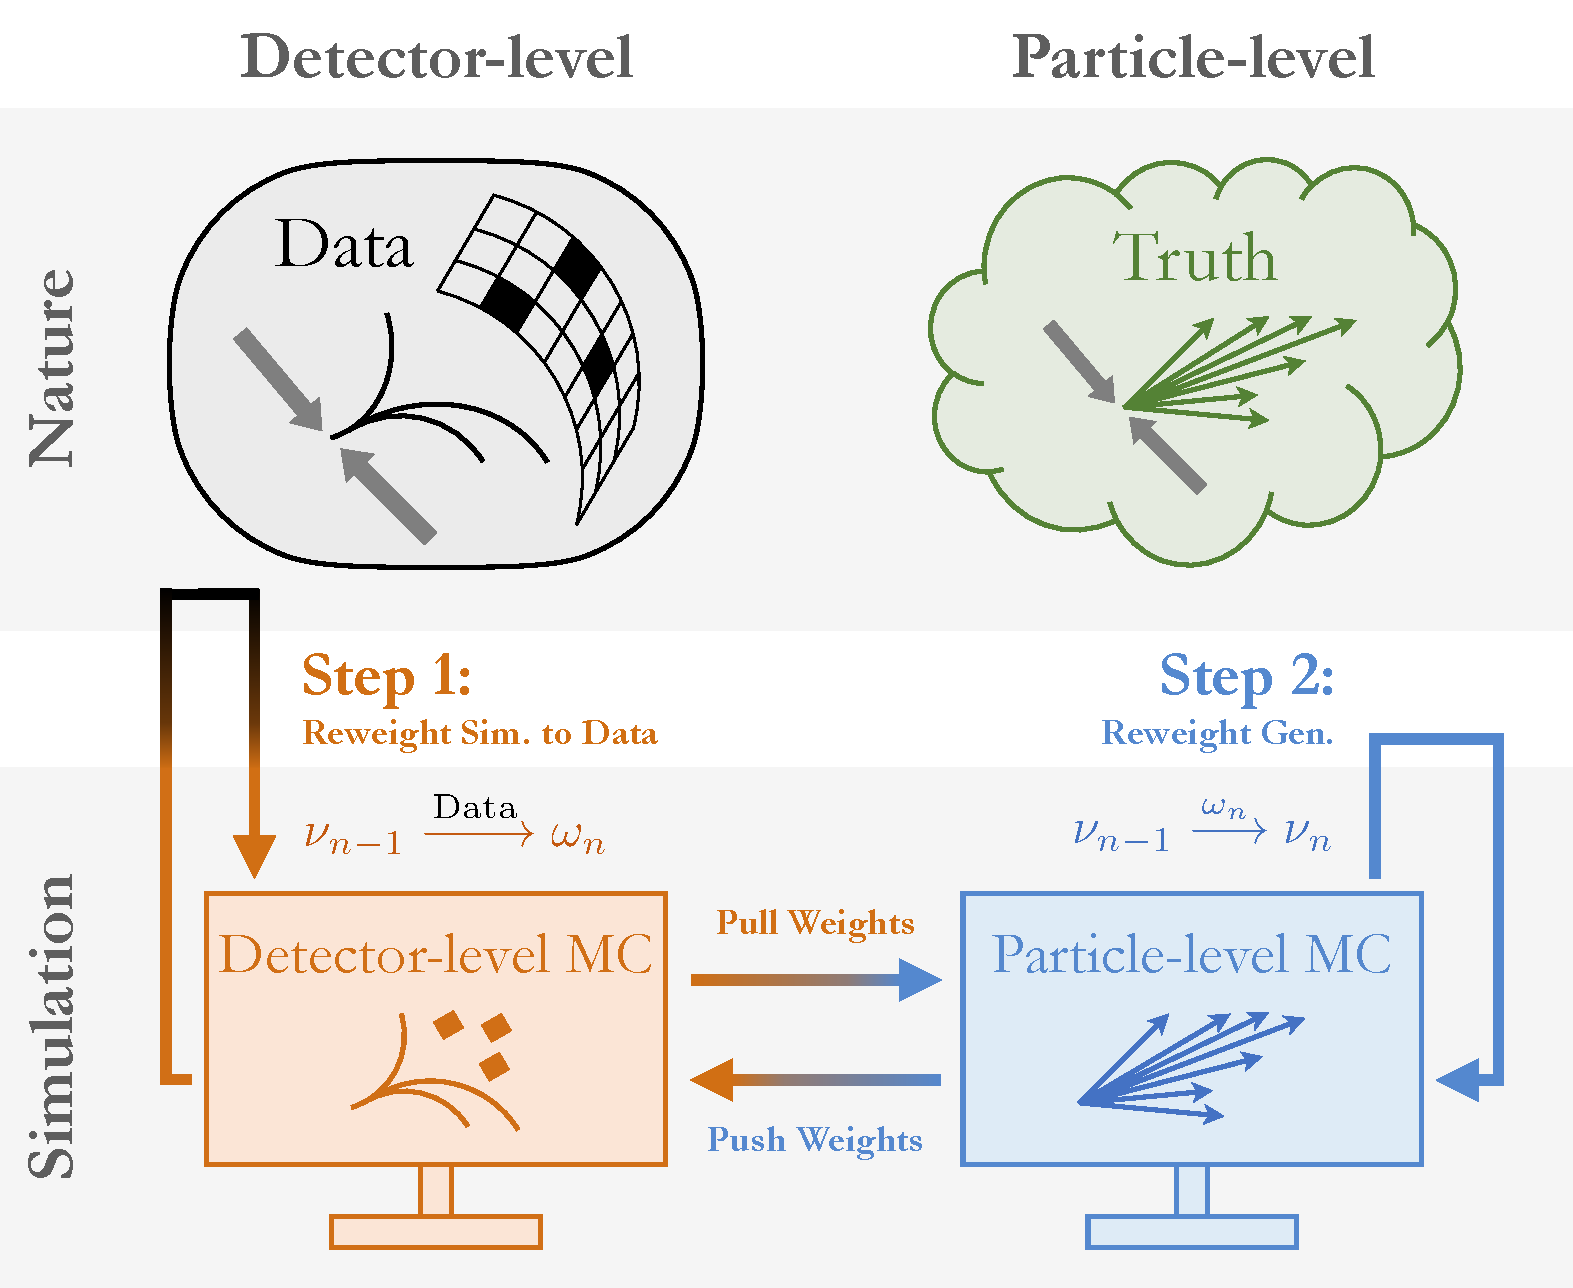
\includegraphics[width=0.6\textwidth]{Figures/schematic.pdf}
\caption{Figure adapted from Ref.~\cite{1911.09107}.}
\label{fig:omnifoldschematic}
\end{figure}

An effective strategy for implementing the OmniFold protocol is to use neural networks as reweighting functions.  A reweighting function is simply a ratio of two probability densities.  It is a fact that the optimal classifier between two event samples is the same quantity - the likelihood ratio (or any monotonic function of it).  Therefore, we build a reweighting function by training a classifier and properly interpreting the output.
In particular, a classifier $f$ trained using the standard binary cross entropy loss function on events with features $\vec{x}_i$ and event weights $w_i$
%
\begin{align}
\label{eq:binarycrossentropy}
        f^*=\argmin_f~~-\sum_{i\in\text{dataset 1}}w_i \log(f(\vec{x}_i)) -\sum_{i\in\text{dataset 2}} w_i\log(1-f(\vec{x}_i)),
\end{align}
%
has the property\footnote{This fact is well-known~\cite{hastie01statisticallearning,sugiyama_suzuki_kanamori_2012} and also has been used in many contexts in high-energy physics~\cite{2010.03569,1907.08209,Stoye:2018ovl,Hollingsworth:2020kjg,Brehmer:2018kdj,Brehmer:2018eca,Brehmer:2019xox,Brehmer:2018hga,Cranmer:2015bka,Badiali:2020wal,Andreassen:2020nkr,Andreassen:2019cjw,Fischer-ACAT2019}.} that asymptotically (i.e.\ with enough training data, flexible enough network architecture and training):
%
\begin{align}
\frac{f^*(\vec{x})}{1-f^*(\vec{x})}\propto \frac{p(\vec{x}|\text{dataset 1})}{p(\vec{x}|\text{dataset 2})}.
\end{align}
%
The proportionality is equality if the two datasets contain the same number of events; however, a constant is not important from the point of view of reweighting.

The power of neural networks is that they are naturally unbinned and can process high-dimensional data.  Furthermore, neural networks can also process variable-length data.  We will refer to the case that the inputs are one-dimensional as UniFold, the case that the inputs are multi- (but fixed-)dimensional as MultiFold, and the case where there are of variable dimension (namely, the raw particle data) as OmniFold.  If it is clear from context, we will simply refer to all of these approaches as OmniFold.

To develop an intuition for how OmniFold operates, the next section compares various approaches in a two-bin example where it is easy to derive the steps analytically.  Following that, we show a Gaussian example where the power of the neural network becomes clear.

\subsubsection{Illustration of Different Methods}

In order to illustrate the OmniFold procedure and how it compares to other techniques, it is useful to consider a simple two-bin example.  Suppose that there are only two possible values at particle-level and detector-level: $(T_1,T_2)$ and $(R_1,R_2)$, respectively.  The random variable $T_i$ is the number of events with a value $i$ at particle level (and similarly for $R_i$).  Further suppose that the detector response is given by:
%
\begin{align}
\Pr(R_1|T_1)&=100\%\,,\\
\Pr(R_1|T_2)&=50\%\,,
\end{align}
%
where $\Pr(x|y)$ is the conditional probability of $x$ given $y$.  The simulation has probability mass $\Pr_\text{MC}(T_i)=50\%$ so that $\Pr_\text{MC}(R_1)=75\%$ and $\Pr_\text{MC}(R_2)=25\%$.   Finally, we observe $\Pr_\text{Data}(R_1)=50\%$ in data.
With the notation used in Eq.~\ref{eq:foldingequation}, this situation is given by
%
\begin{eqnarray}
	\mathbf{R} = \begin{bmatrix} 1 & 0.5\\ 0 & 0.5\end{bmatrix}, & \mathbf{d} = \begin{bmatrix} 0.5\\ 0.5\end{bmatrix}, & \mathbf{c}=\mathbf{f}=\mathbf{1},~~\mathbf{b}=\mathbf{0}.
\end{eqnarray}
%
What do the various method predict for $\Pr_\text{unfolded}(T_1)$?   Before proceeding, note that the correct answer is $\Pr_\text{Data}(T_1)=0$, i.e.\ $\mathbf{t}=[0 1]^\intercal$.

\paragraph{OmniFold}  The first step of OmniFold is to derive weights $\omega_1$ to make the MC match the data.  The weight function is specified by two numbers, one for each of the two bin values.  These weights are given by $\omega_1(R_i)=\Pr_\text{Data}(R_i)/\Pr_\text{MC}(R_i)$, which is $\omega_1(R_1)=2/3$ and $\omega_1(R_2)=2$.  These weights are then pulled back to particle level.  In MC, 50\% of events have $(T_1,R_1)$, 25\% of events have $(T_2,R_1)$ and 25\% of events have $(T_2,R_2)$.   The first two of these types of events get assigned $\omega(R_1)$ and the last one gets assigned $\omega(R_2)$.  Therefore, the weighted particle-level probability mass function is $\Pr_\text{MC,1}(T_1)=1/3$.  The second step of OmniFold derives weights $\nu_1=\Pr_\text{MC,1}(T_i)/\Pr_\text{MC}(T_i)$, which are $\nu_1(T_1)=2/3$ and $\nu_1(T_2)=4/3$.

The above procedure is then repeated using the weights $\nu_1$ pushed to detector-level.  The new detector-level probability mass is given by $\Pr_\text{MC,2}(R_1)=2/3$.  Detector-level weights are derived according to $\omega_2(R_i)=\Pr_\text{Data}(R_i)/\Pr_\text{MC,2}(R_i)$.  Table~\ref{lab:omnifoldexample} shows the evolution of OmniFold over many iterations.

\begin{table}[h!]
\centering
\begin{tabular}{|ccccccc| }
\hline
$i$ & $\omega_i(R_1)$ & $\omega_i(R_2)$ & $\nu_i(R_1)$ & $\nu_i(R_2)$ & $\Pr_\text{MC,$i$}(R_1)$ & $\Pr_\text{MC,$i$}(T_1)$ \\
\hline
0 & 1 & 1 & 1 & 1 & $\sfrac{3}{4}$ & $\sfrac{1}{2}$ \\
1 & $\sfrac{2}{3}$ & $2$ & $\sfrac{2}{3}$ & $\sfrac{4}{3}$ & $\sfrac{2}{3}$ & $\sfrac{1}{3}$ \\
2 & $\sfrac{3}{4}$ & $\sfrac{3}{2}$ & $\sfrac{1}{2}$ & $\sfrac{3}{2}$ & $\sfrac{5}{8}$ & $\sfrac{1}{4}$ \\
\vdots & \vdots & \vdots & \vdots & \vdots & \vdots & \vdots \\
$\infty$ & 1 & 1 & 0 & 2 & \sfrac{1}{2} & 0\\
\hline
\end{tabular}
\caption{The evolution of OmniFold for the simple two-bin example described in the text.}
\label{lab:omnifoldexample}
\end{table}

\paragraph{Conditional GAN Unfolding (CGU)} In the training phase of CGU, one learns $\Pr(T_i|R_j)$ based on the simulation.  In the simple binned case, this probability mass is specified by four numbers.

\begin{align}
\Pr(T_i|R_j)&=\frac{\Pr(R_j|T_i)\Pr(T_i)}{\Pr(R_j|T_1)\Pr(T_1)+\Pr(R_j|T_2)\Pr(T_2)}\\
&=\frac{\Pr(R_j|T_i)}{\Pr(R_j|T_1)+\Pr(R_j|T_2)}\\
&=\left\{\begin{matrix}\sfrac{2}{3} & \text{$i=1$ and $j=1$} \cr 0 & \text{$i=1$ and $j=2$}  \cr \sfrac{1}{3}& \text{$i=2$ and $j=1$}  \cr 1& \text{$i=2$ and $j=2$}  \end{matrix}\right.
\end{align}
%
Applied to data, we would measure
%
\begin{align}
\Pr{}_\text{unfolded}(T_1)&=\Pr(T_1|R_1)\Pr{}_\text{data}(R_1)+\Pr(T_1|R_2)\Pr{}_\text{data}(R_2)=\sfrac{1}{6}\,,\\
\Pr{}_\text{unfolded}(T_2)&=\Pr(T_2|R_1)\Pr{}_\text{data}(R_1)+\Pr(T_2|R_2)\Pr{}_\text{data}(R_2)=\sfrac{5}{6}\,,
\end{align}
%
which is the wrong answer.

\paragraph{Conditional Normalizing Flow Unfolding (CNFU)} In the binned case, this is equivalent to matrix inversion.   The response matrix is

\begin{align}
\mathbf{R}=\begin{pmatrix} 1& \sfrac{1}{2}\cr 0 & \sfrac{1}{2}\end{pmatrix}\implies \mathbf{R}^{-1}=\begin{pmatrix} 1 & -1 \cr 0 & 2\end{pmatrix}\,.
\end{align}
%
Applying $\mathbf{R}^{-1}$ to $(\sfrac{1}{2},\sfrac{1}{2}$) results in $(0,1)$, the correct answer.  There are many undesirable features of matrix inversion, but it does result in an unbiased measurement.

\paragraph{Iterative Bayesian Unfolding (IBU)}

Table~\ref{lab:ibuexample} shows the evolution of IBU over many iterations.  Note that the second column of Table~\ref{lab:ibuexample} is the same as the last column of Table~\ref{lab:omnifoldexample} - this is because OmniFold and IBU are equivalent in the binned case.

\begin{table}[h!]
\centering
\begin{tabular}{|cccccc| }
\hline
$i$ & $\Pr_\text{MC,$i$}(T_1)$ & $\Pr_0(T_1|M_1)$ & $\Pr_0(T_1|M_2)$ & $\Pr_0(T_2|M_1)$ & $\Pr_0(T_2|M_2)$\\
\hline
$0$ & $\sfrac{1}{2}$ & $\sfrac{2}{3}$ & 0 & $\sfrac{1}{3}$ & $1$\\
$1$ & $\sfrac{1}{3}$ & $\sfrac{1}{2}$ & 0 & $\sfrac{1}{2}$ & $1$\\
$2$ & $\sfrac{1}{4}$ & $\sfrac{2}{5}$ & 0 & $\sfrac{3}{5}$ & $1$\\
\vdots & \vdots & \vdots & \vdots & \vdots & \vdots  \\
$\infty$ & 0 & 0 & 0 & 1 & 1\\
\hline
\end{tabular}
\caption{The evolution of IBU for the simple two-bin example described in the text.}
\label{lab:ibuexample}
\end{table}

\subsection{Gaussian Example}
\label{sec:gaus}

This section shows the unfolding of a one-dimensional Gaussian random variable with a Gaussian noise model.  Figure~\ref{fig:gaussian:inputs} shows the `data' and `simulation'.  The data has a mean of 1 and a standard deviation of 1.5 while the simulation has a mean of 0 and a standard deviation of 1.  In both cases, the distributions are made up of ten million events and the detector effects (noise) are an additive Gaussian with mean 0 and unit variance.

The neural network implemented for reweighting is comprised of 3 layers, with 50 nodes per layer.  Rectified linear units (ReLU) connect the intermediate layers and the output is Softmax.  The training/validation split is 75/25.  The network is trained for 200 epochs with early stopping using a patience of 10\footnote{The training ends if the validation loss is not improved for 10 epochs.  The network weights with the lowest validation loss are restored.}, and the training time is about 5 seconds per epoch on an NVIDIA Quadro RTX 6000 GPU. The batch size is $10^5$.  All neural networks are implemented using \textsc{Keras}~\cite{keras} with the \textsc{Tensorflow} backend~\cite{tensorflow} and optimized with \textsc{Adam}~\cite{adam}.  Networks are trained using the binary cross entropy loss function described in Eq.~\ref{eq:binarycrossentropy}.

Six iterations resulting in successful unfolding using the OmniFold procedure is demonstrated in Fig.~\ref{fig:gaussian:iterations}.

To model the effects of initial Monte Carlo (MC) generation event weights, we inject artificial initial event weights. Specifically, each event in the particle-level truth and particle-level simulation $x_i$ is given a weight $w_i$ with $w_i$ drawn from $\mathcal{N}(x_i, 1)$; effectively, events further from the origin are more heavily weighted. This results in the distributions shown in Figure~\ref{fig:gaussian:MCinputs}. We then carry out an identical unfolding procedure as described above, simply initializing $\omega_0$ as the initial event weights $w_i$ for simulation.

Again, six iterations resulting in successful unfolding using the OmniFold procedure for the case with initial MC weights injected is demonstrated in Fig.~\ref{fig:gaussian:MCiterations}.

\begin{figure}[h!]
\centering
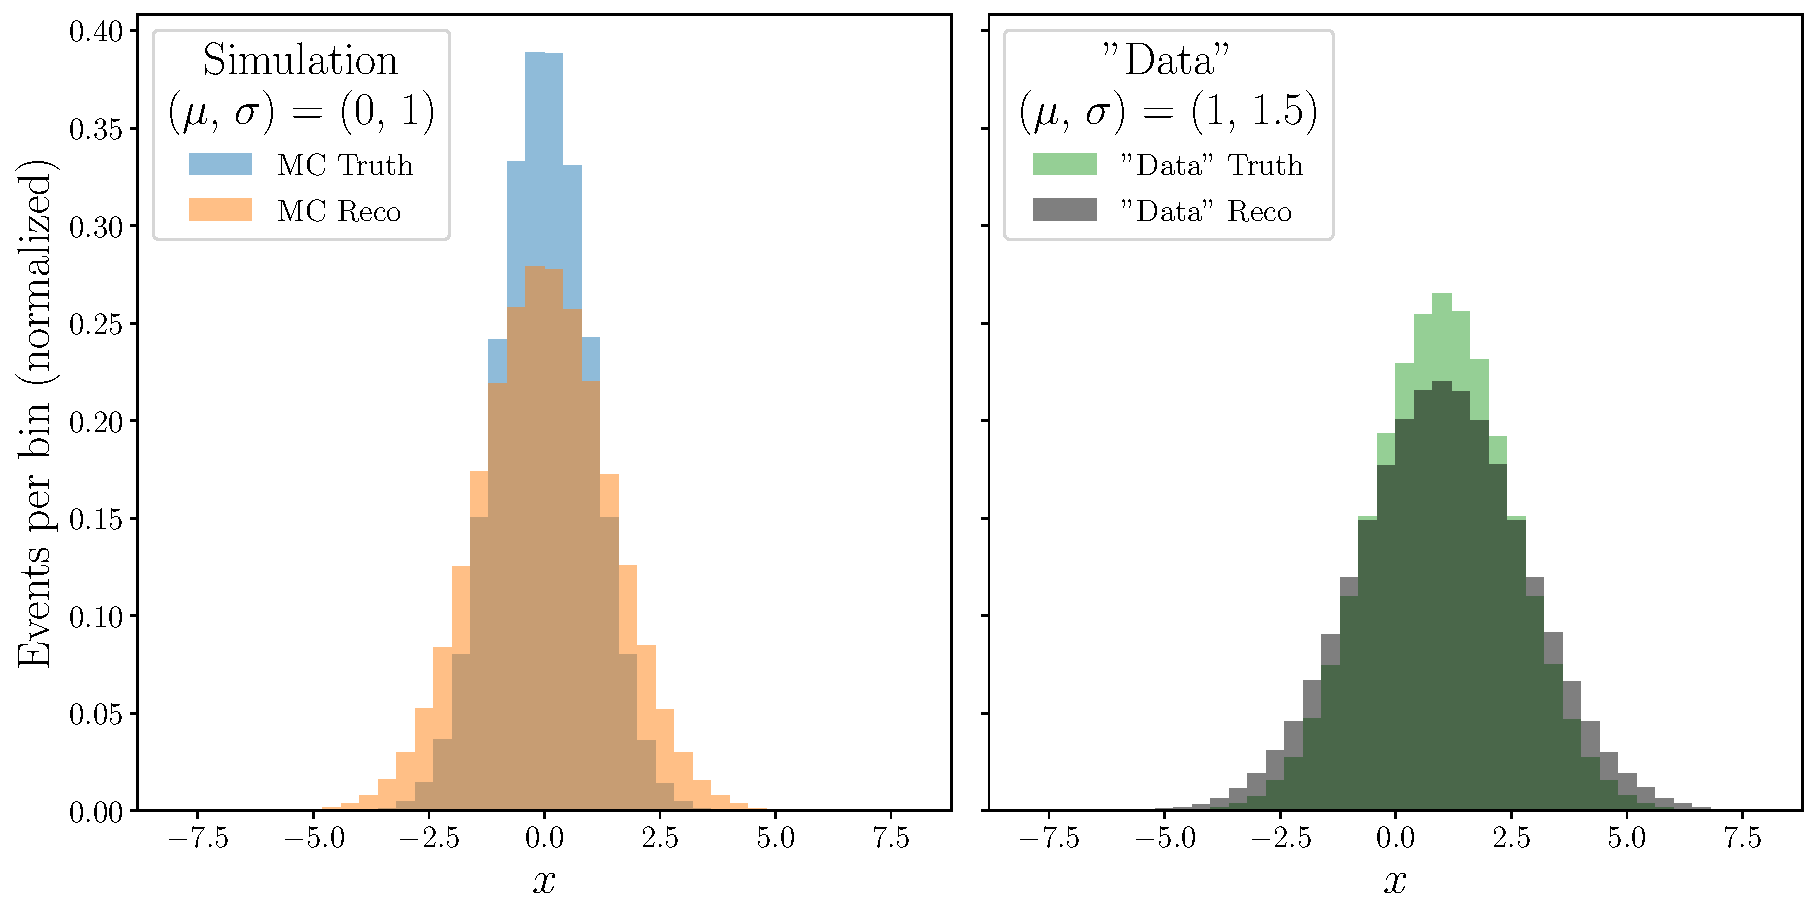
\includegraphics[width=0.6\textwidth]{Figures/GaussianToyExample/GaussianToyExample-Distributions.pdf}
\caption{The `simulation' (left) and `data' (right) for the one-dimensional Gaussian illustration.  The narrower histograms are the particle-level distributions and the wider ones are the detector-level distributions.}
\label{fig:gaussian:inputs}
\end{figure}

\begin{figure}[h!]
\centering
\subfloat[1 iteration]{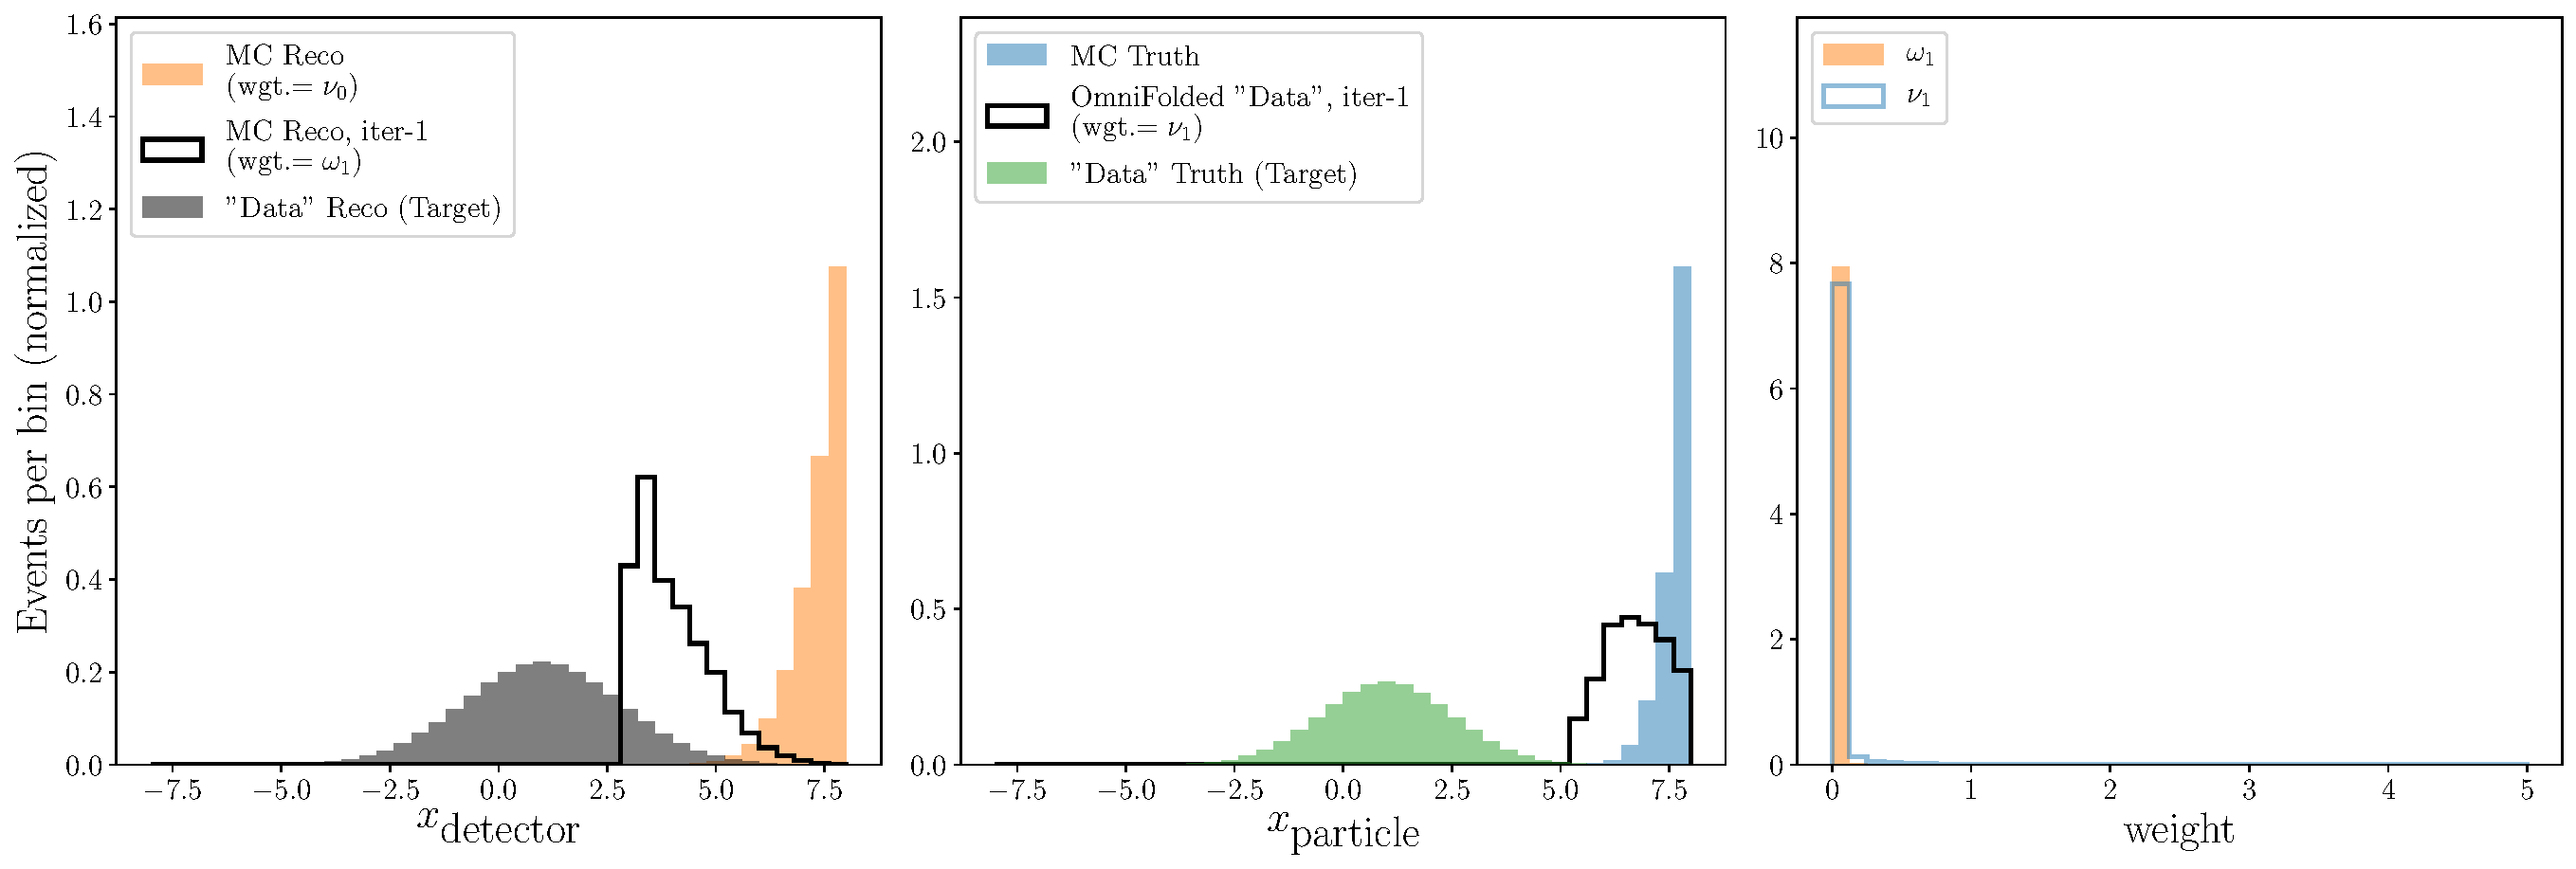
\includegraphics[width=0.45\textwidth]{Figures/GaussianToyExample/GaussianToyExample-UnfoldingResultsIteration01.pdf}}\subfloat[2 iterations]{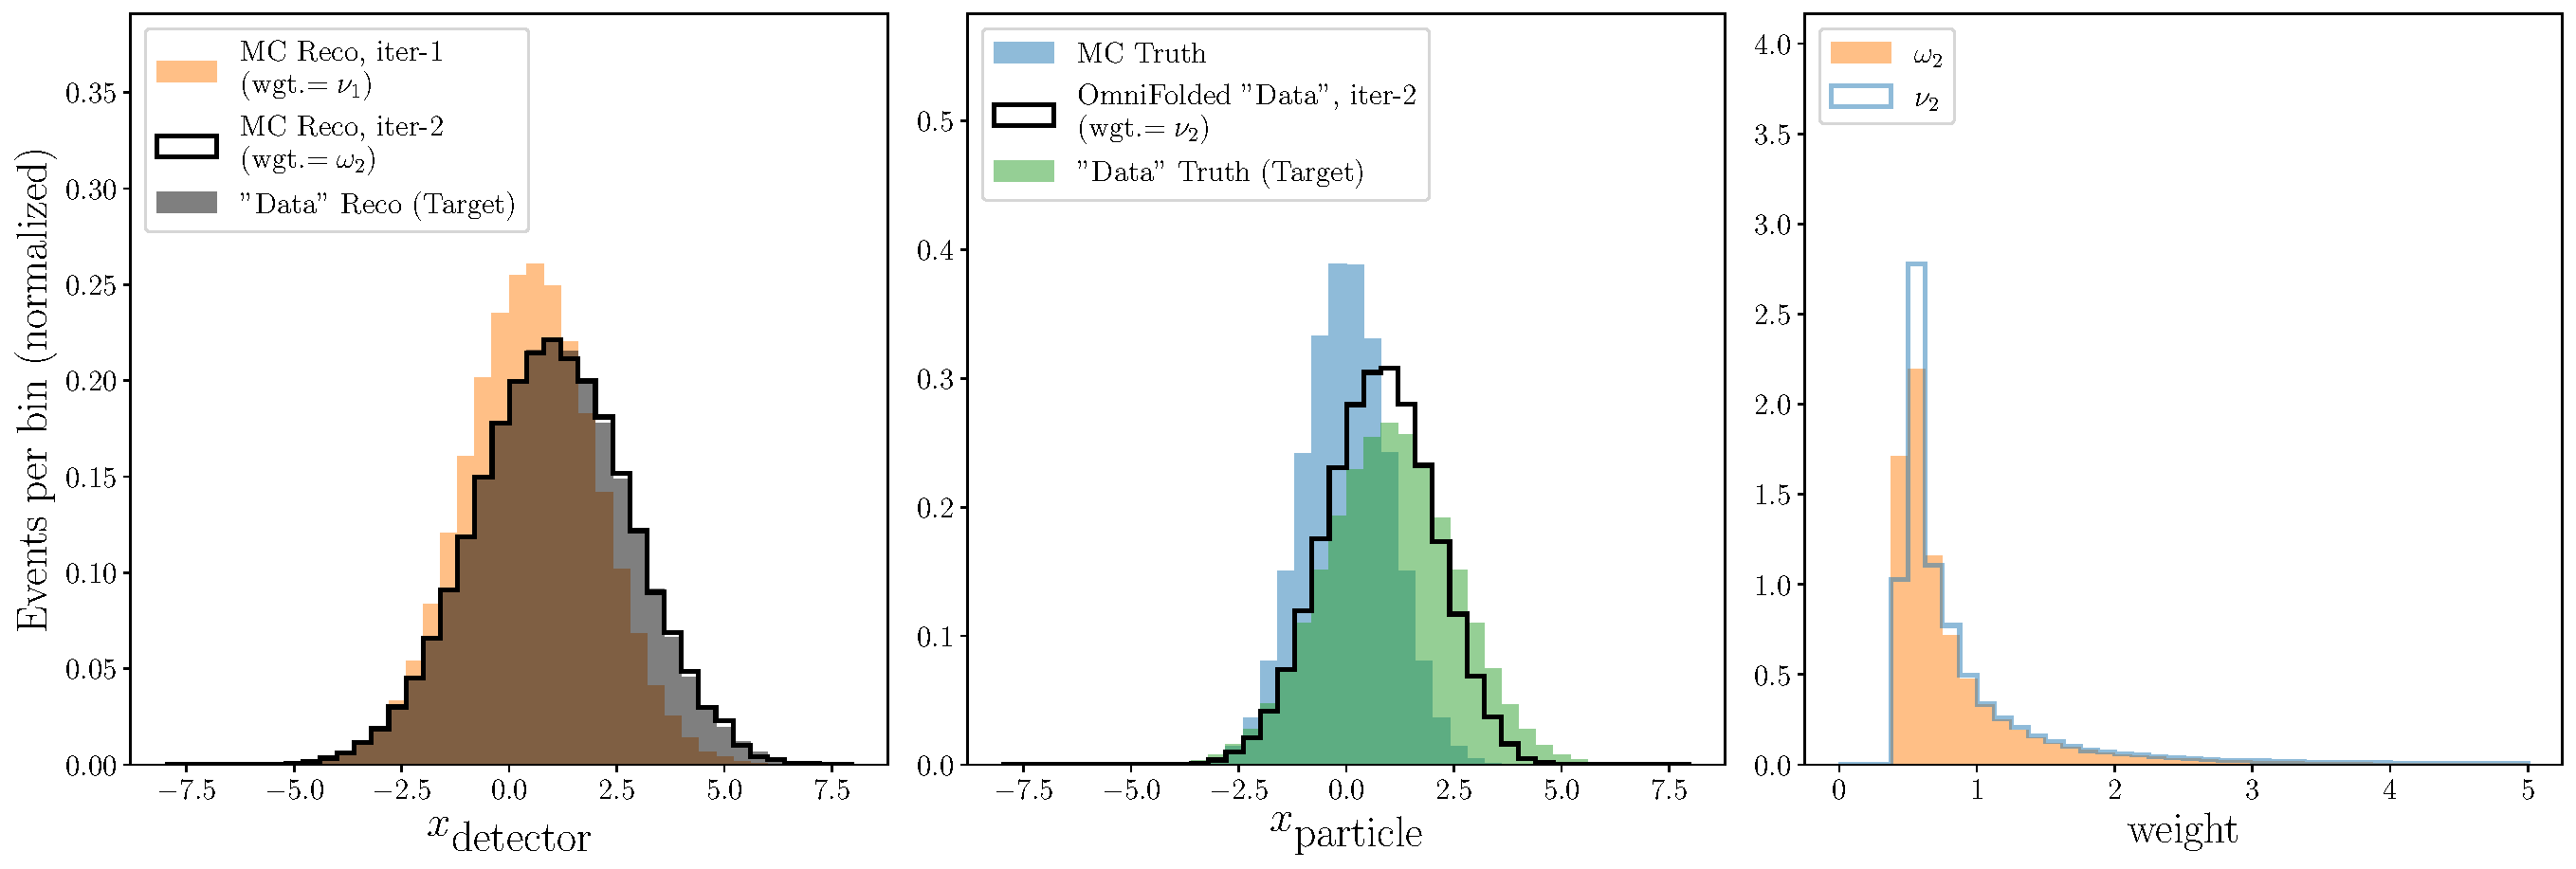
\includegraphics[width=0.45\textwidth]{Figures/GaussianToyExample/GaussianToyExample-UnfoldingResultsIteration02.pdf}}\\
\subfloat[3 iterations]{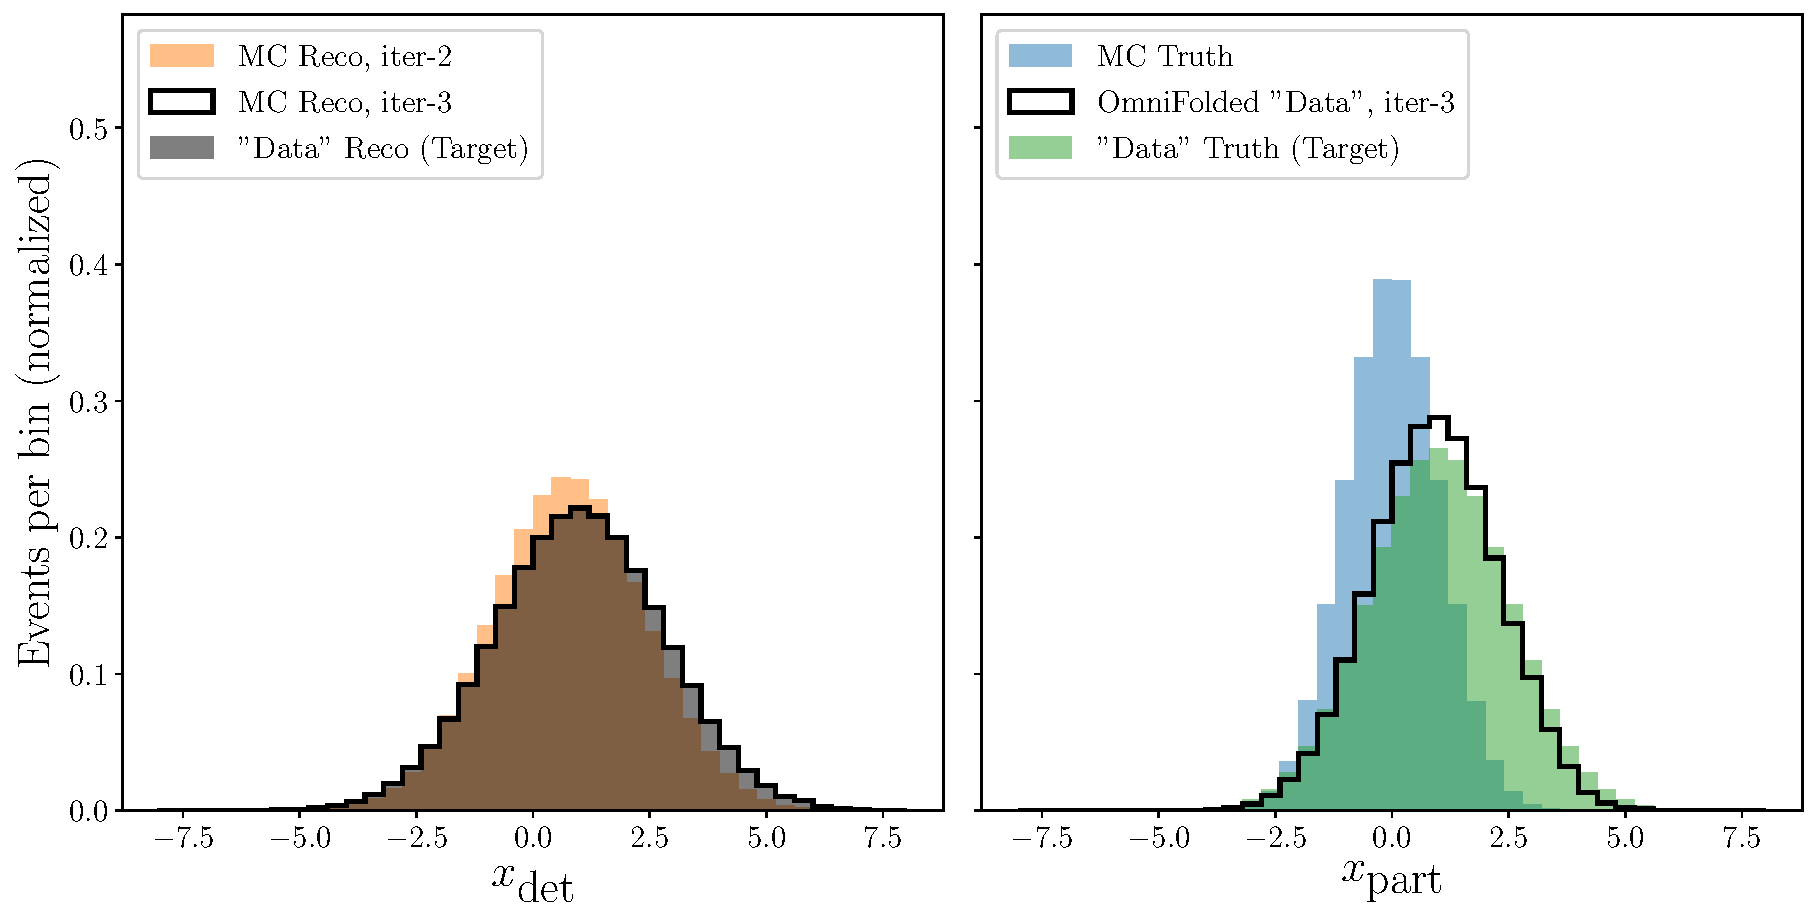
\includegraphics[width=0.45\textwidth]{Figures/GaussianToyExample/GaussianToyExample-UnfoldingResultsIteration03.pdf}}\subfloat[4 iterations]{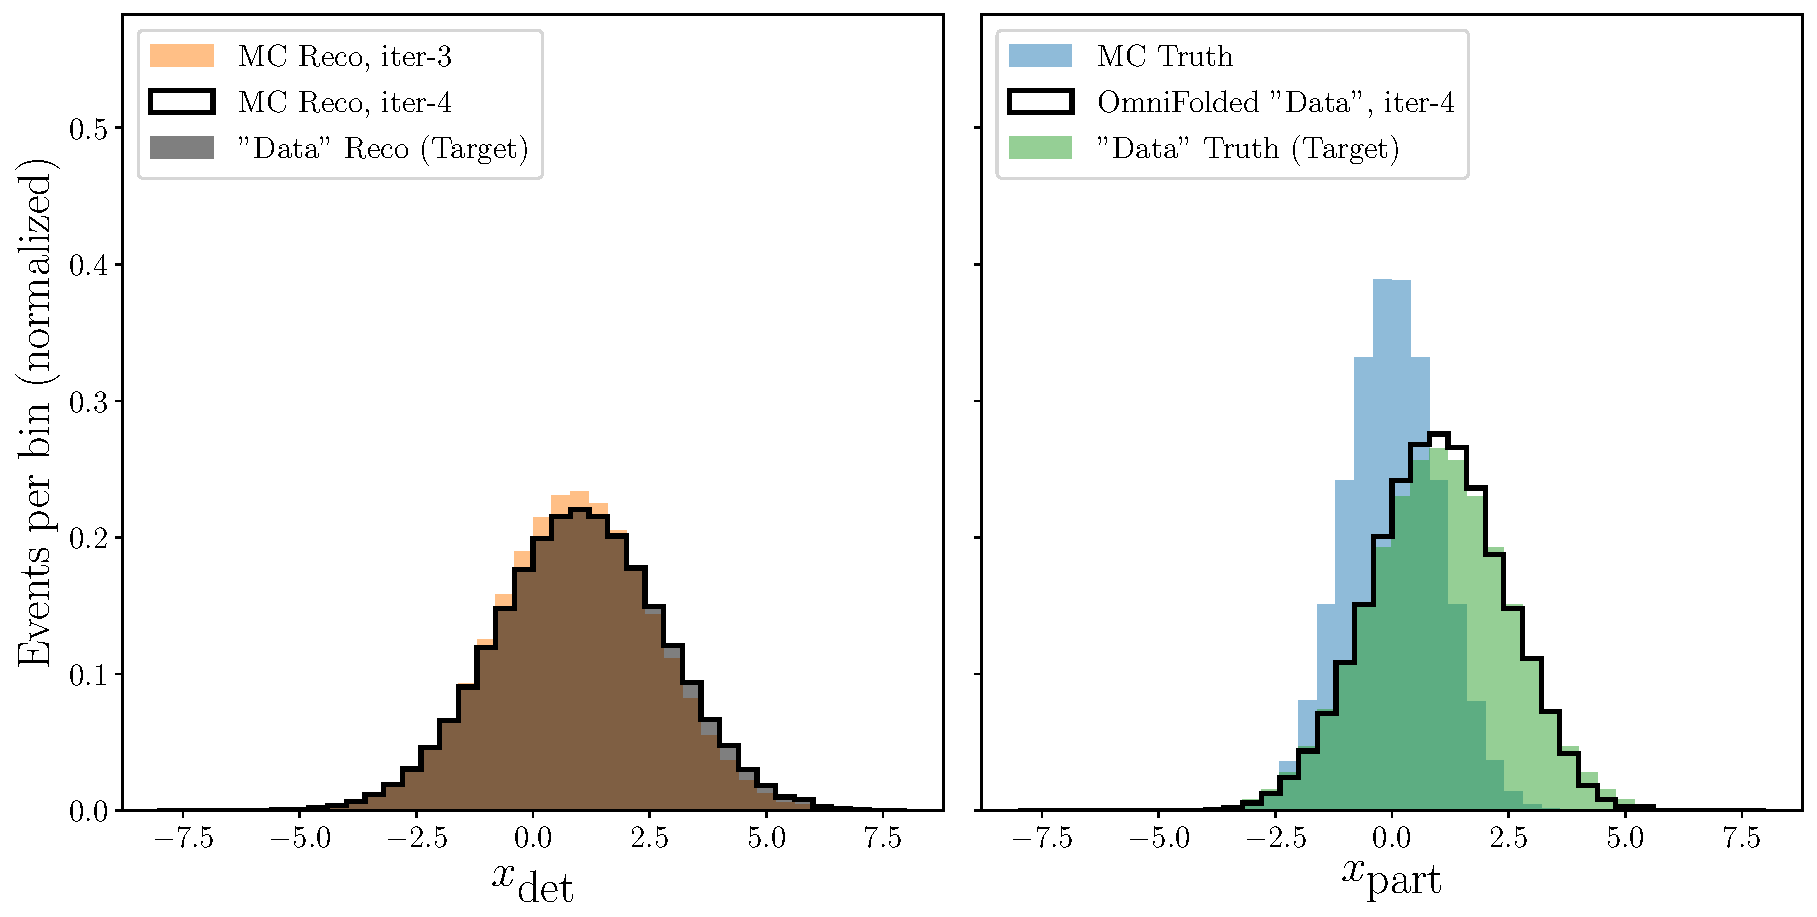
\includegraphics[width=0.45\textwidth]{Figures/GaussianToyExample/GaussianToyExample-UnfoldingResultsIteration04.pdf}}\\
\subfloat[5 iterations]{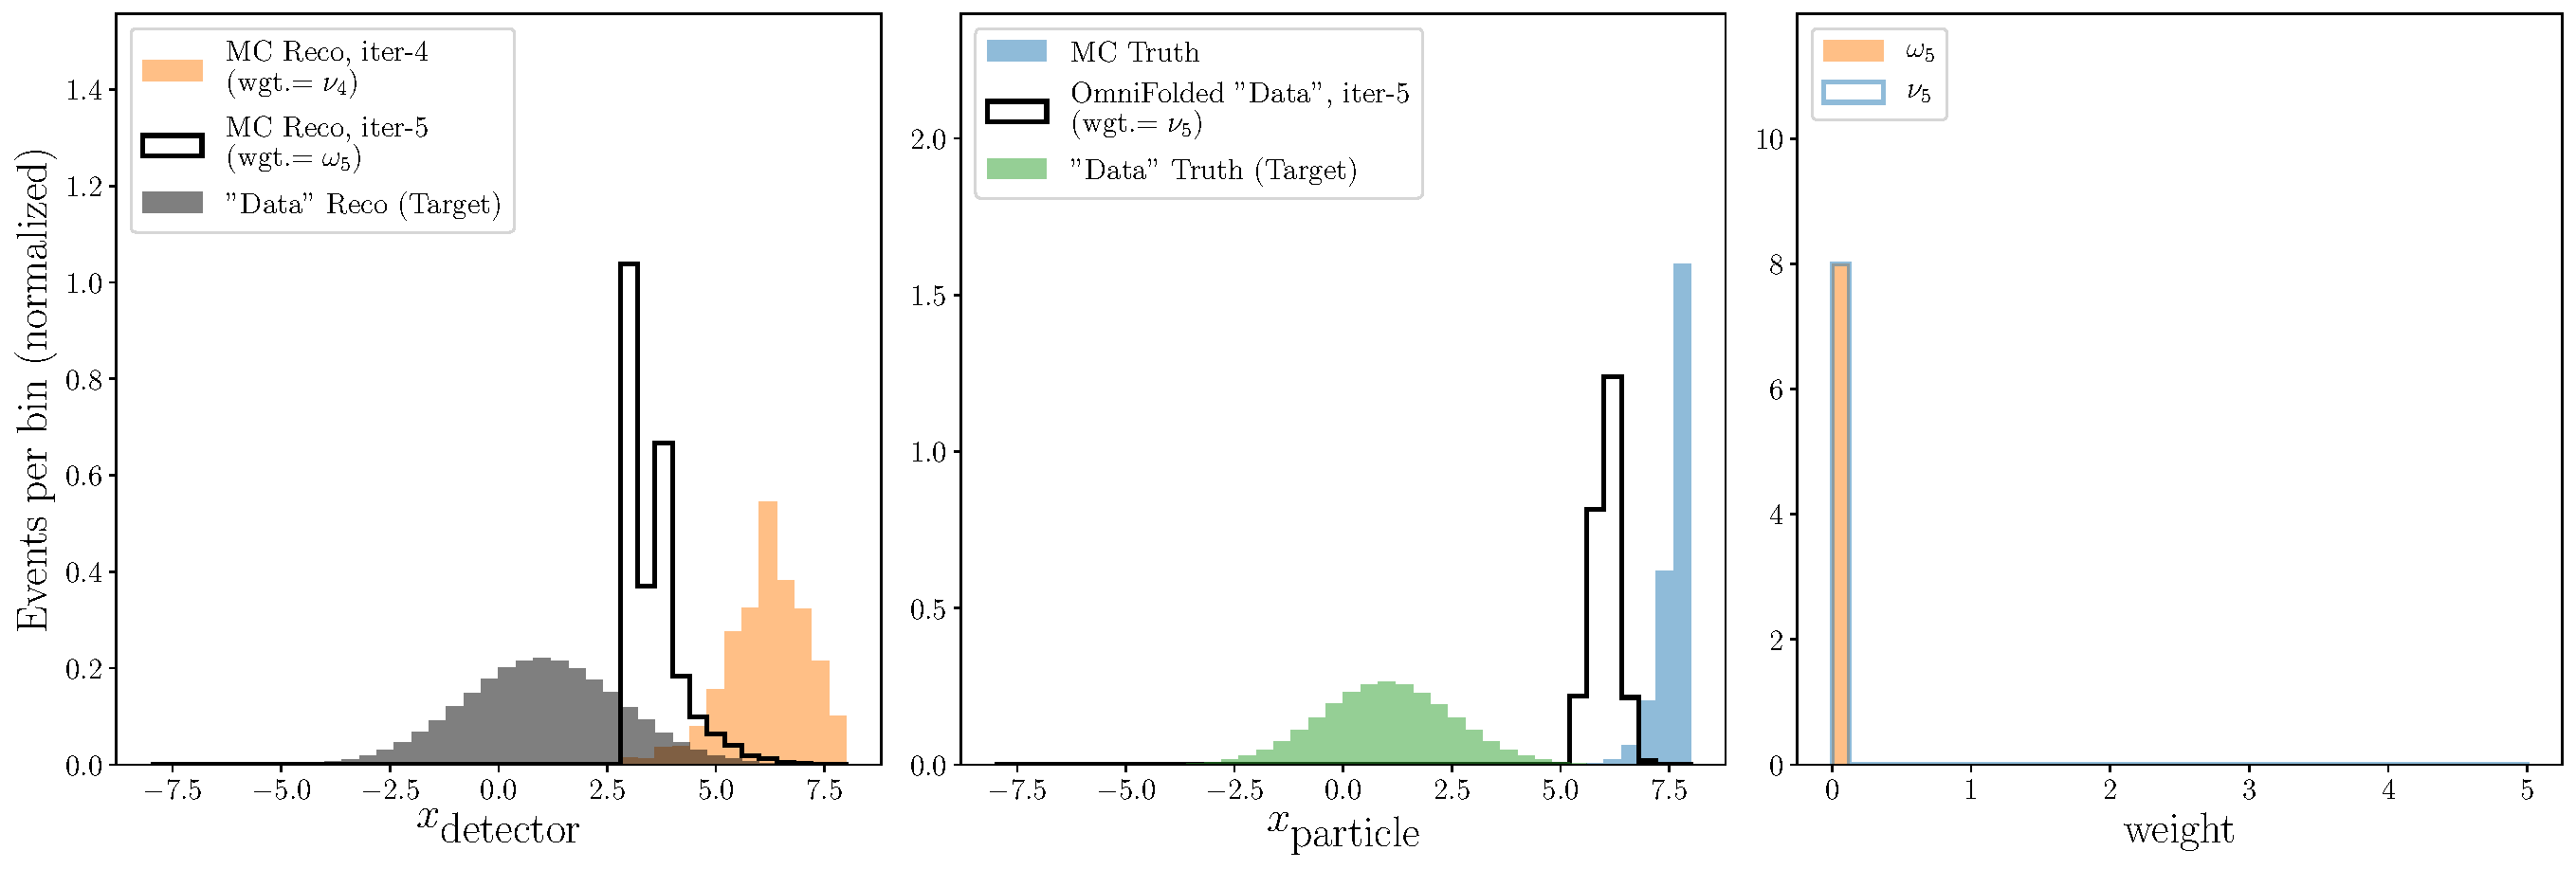
\includegraphics[width=0.45\textwidth]{Figures/GaussianToyExample/GaussianToyExample-UnfoldingResultsIteration05.pdf}}\subfloat[6 iterations]{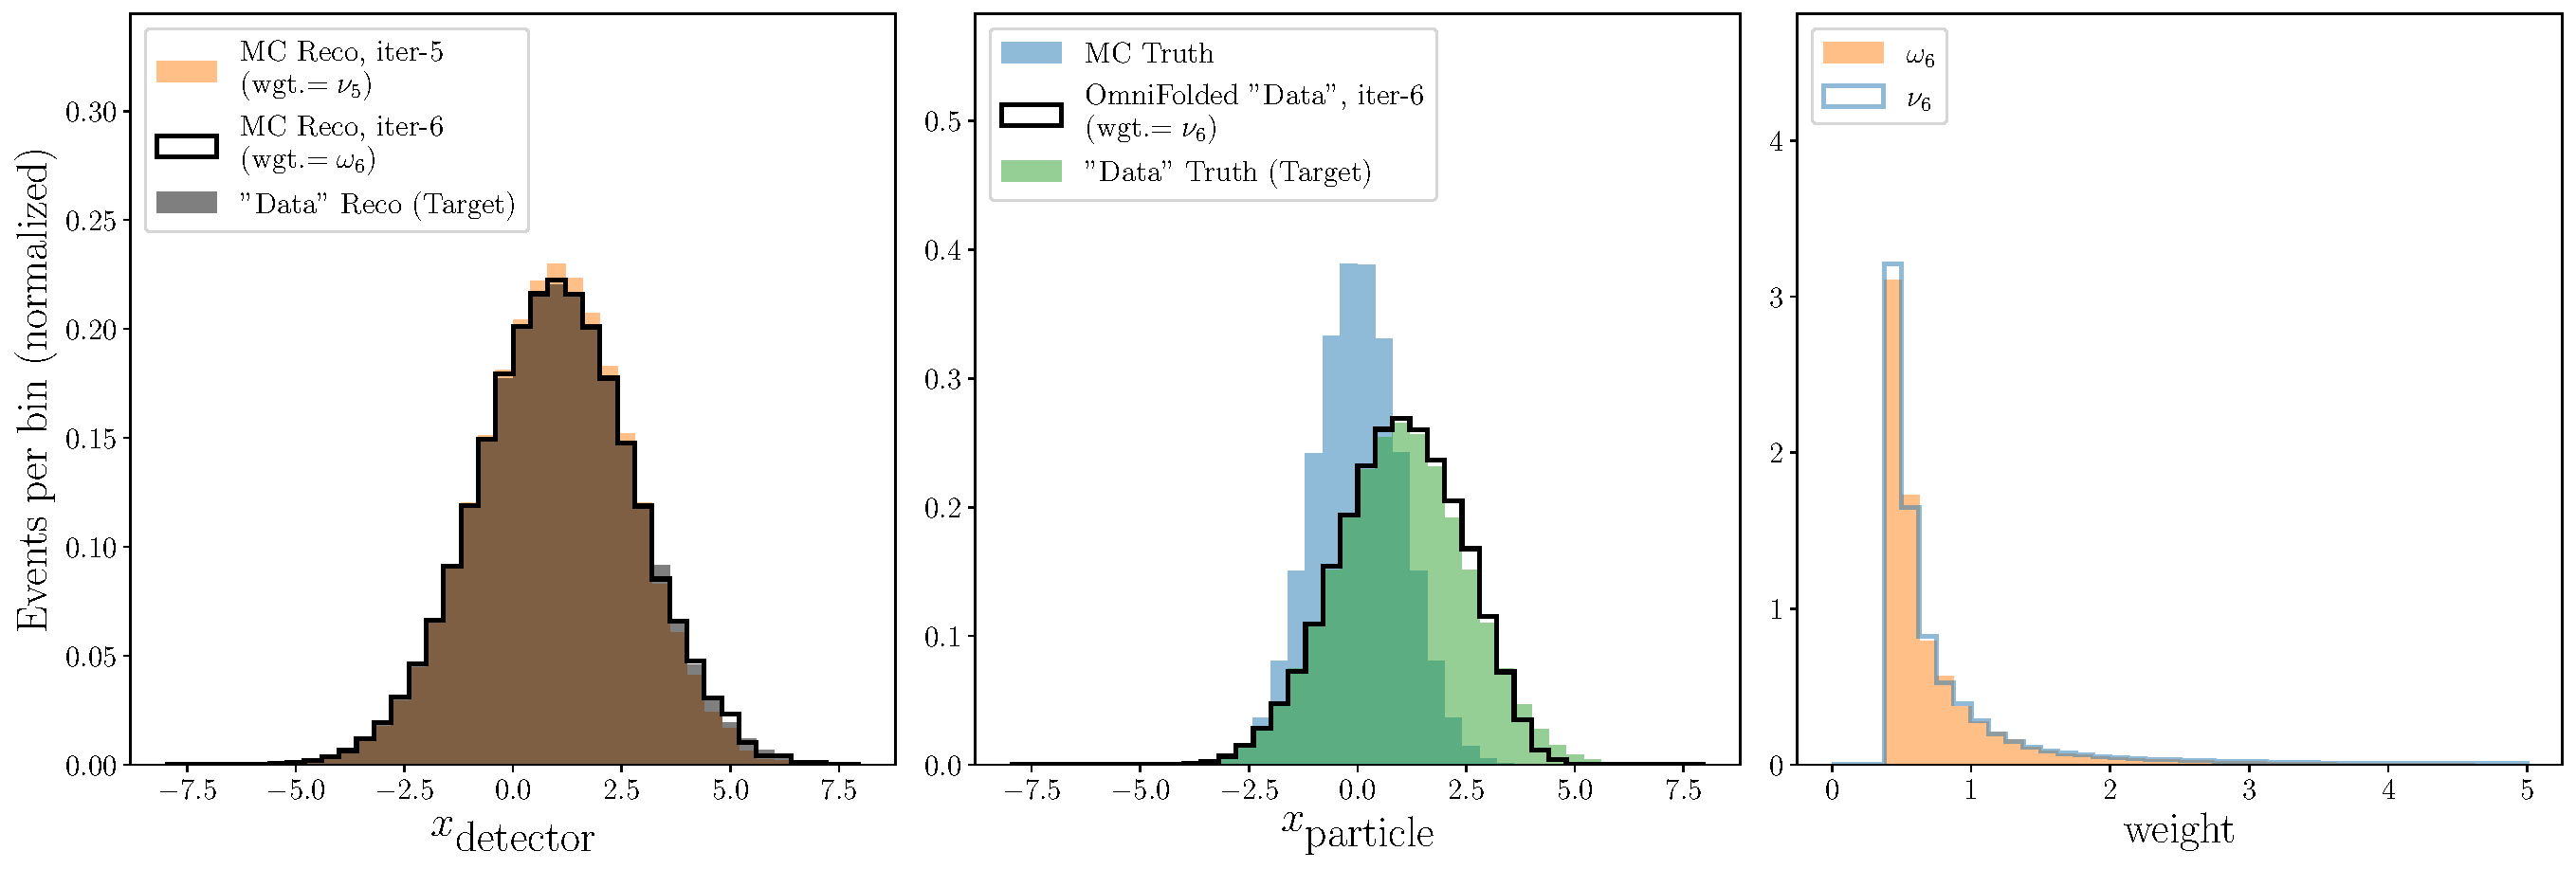
\includegraphics[width=0.45\textwidth]{Figures/GaussianToyExample/GaussianToyExample-UnfoldingResultsIteration06.pdf}}
\caption{An illustration of six iterations of the OmniFold algorithm to the one-dimensional Gaussian example.  For each iteration, the left plot is the detector-level distribution with weights $\omega_n$ and the right plot is the particle-level distribution with weights $\nu_n$.}
\label{fig:gaussian:iterations}
\end{figure}

\begin{figure}[h!]
\centering
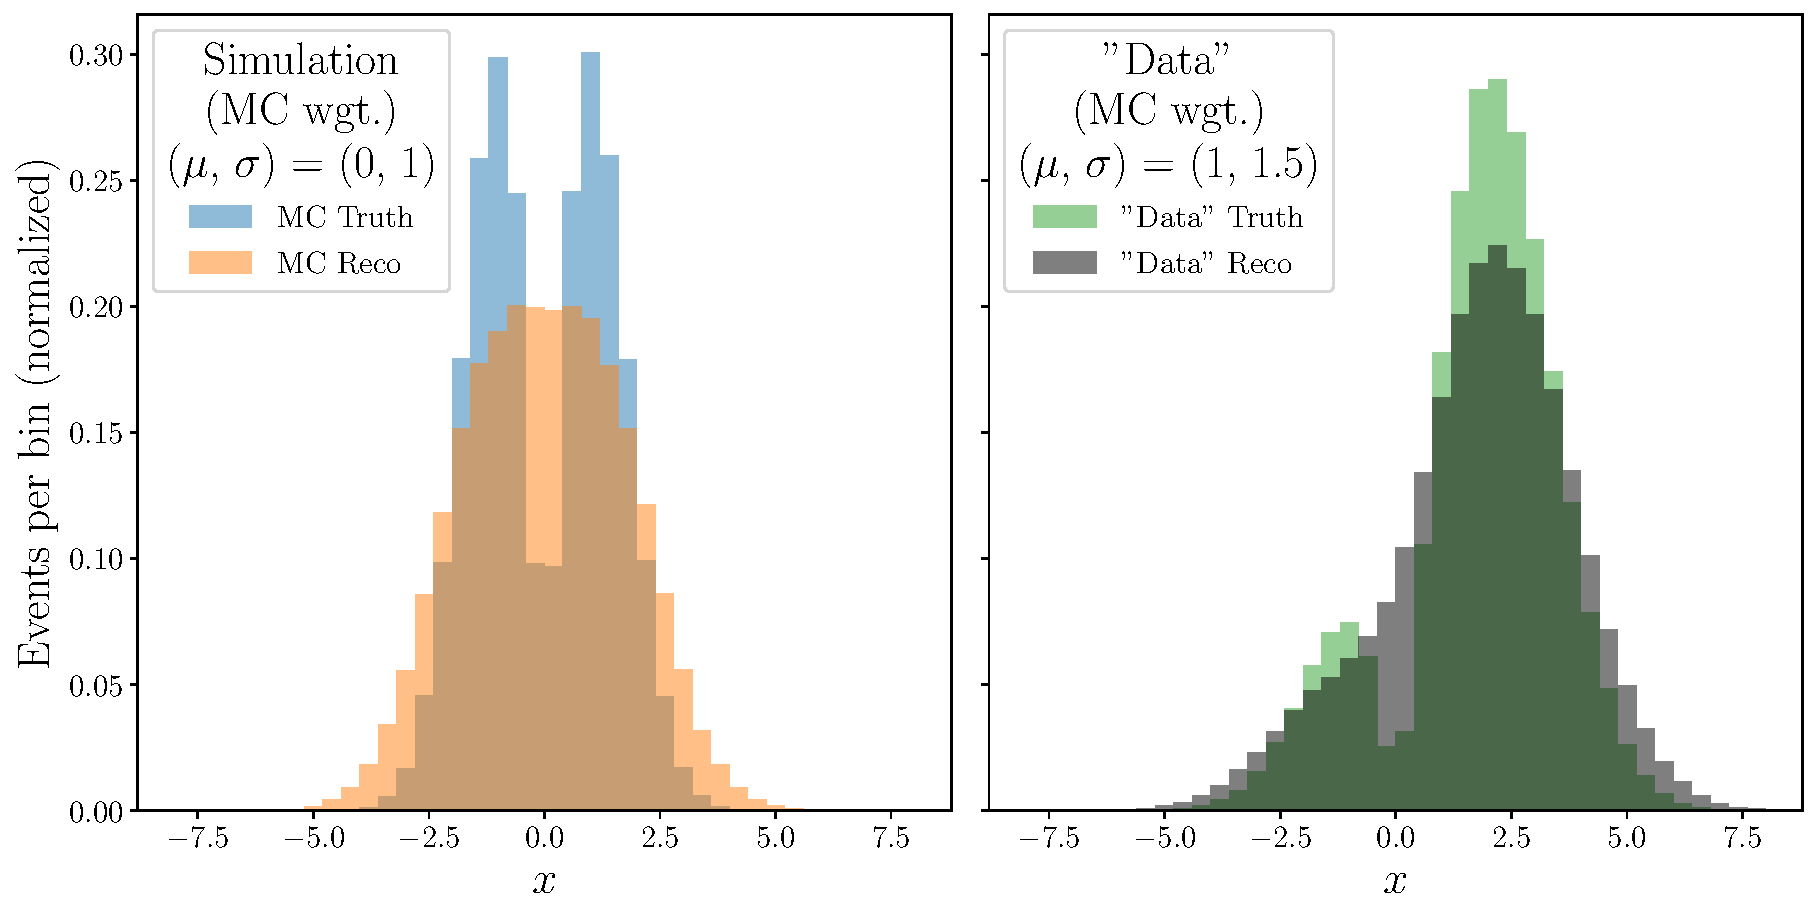
\includegraphics[width=0.6\textwidth]{Figures/GaussianToyExample/GaussianToyExample-MCDistributions.pdf}
\caption{The `simulation' (left) and `data' (right) for the one-dimensional Gaussian illustration with initial MC event weights included.}
\label{fig:gaussian:MCinputs}
\end{figure}

\begin{figure}[h!]
\centering
\subfloat[1 iteration]{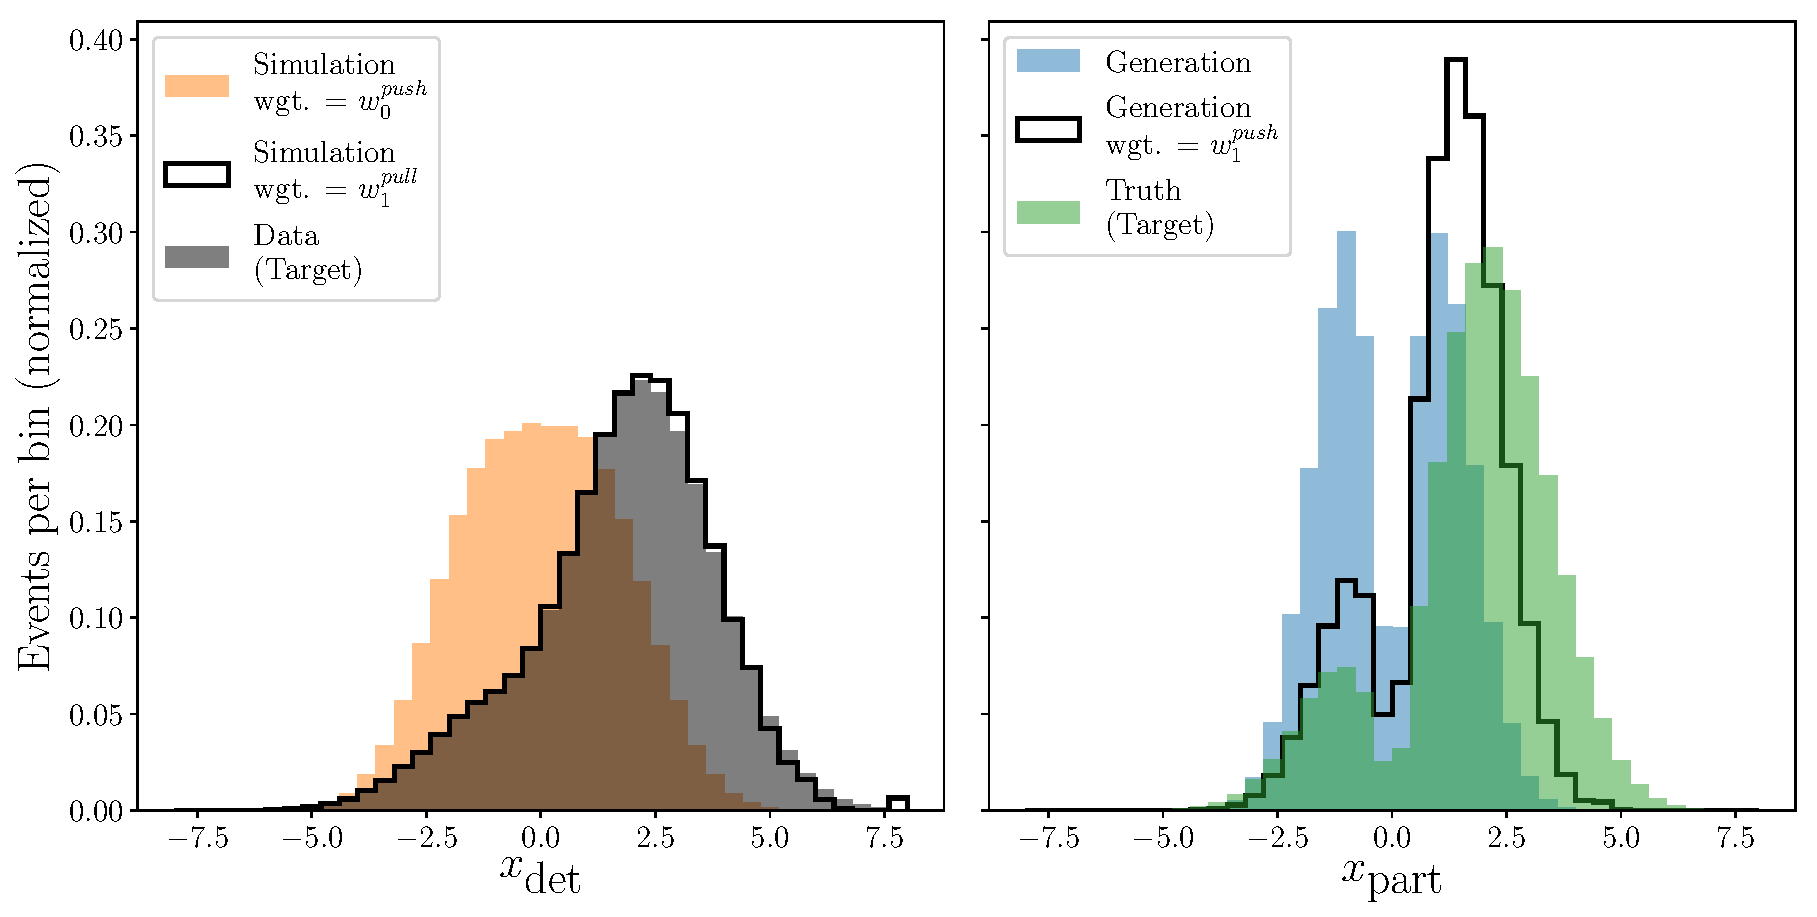
\includegraphics[width=0.45\textwidth]{Figures/GaussianToyExample/GaussianToyExample-MCUnfoldingResultsIteration01.pdf}}\subfloat[2 iterations]{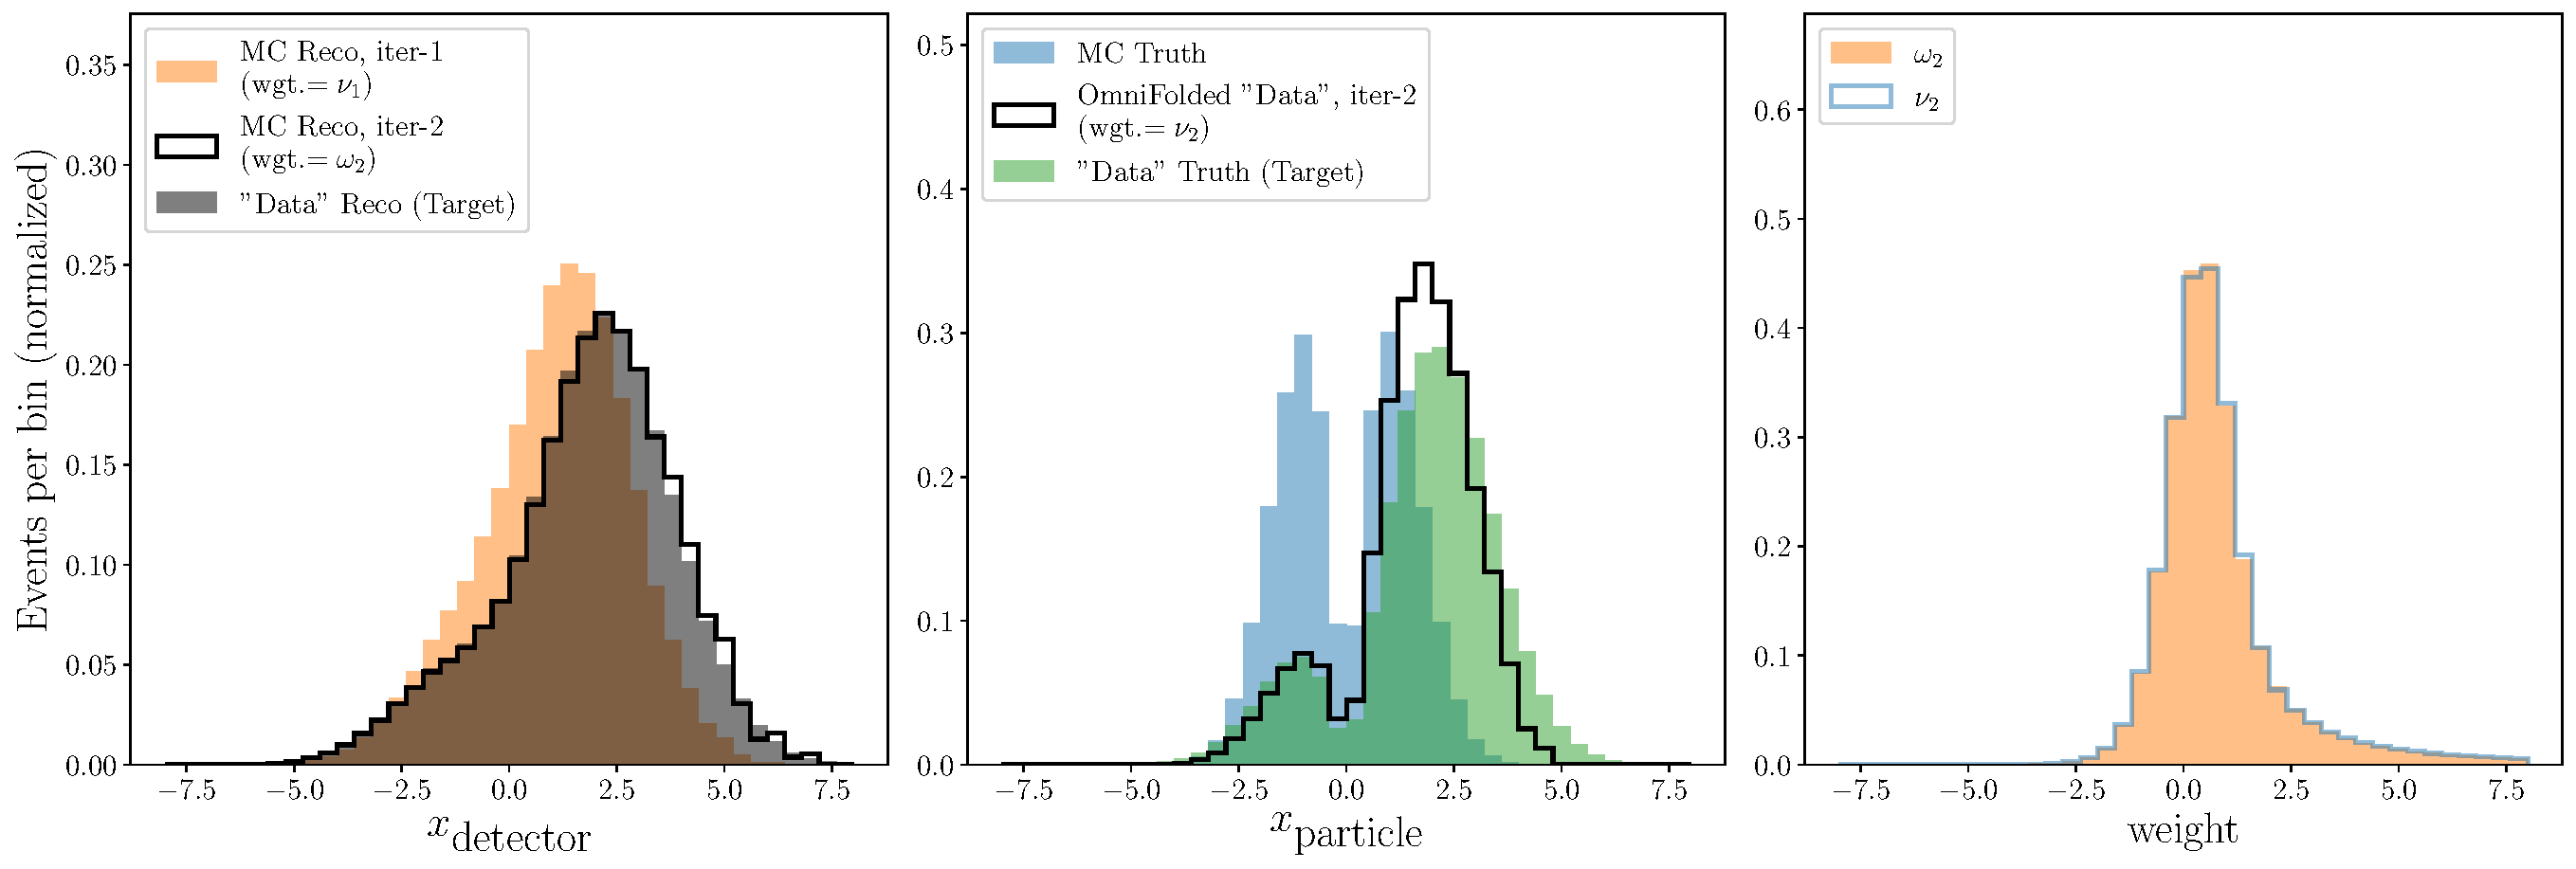
\includegraphics[width=0.45\textwidth]{Figures/GaussianToyExample/GaussianToyExample-MCUnfoldingResultsIteration02.pdf}}\\
\subfloat[3 iterations]{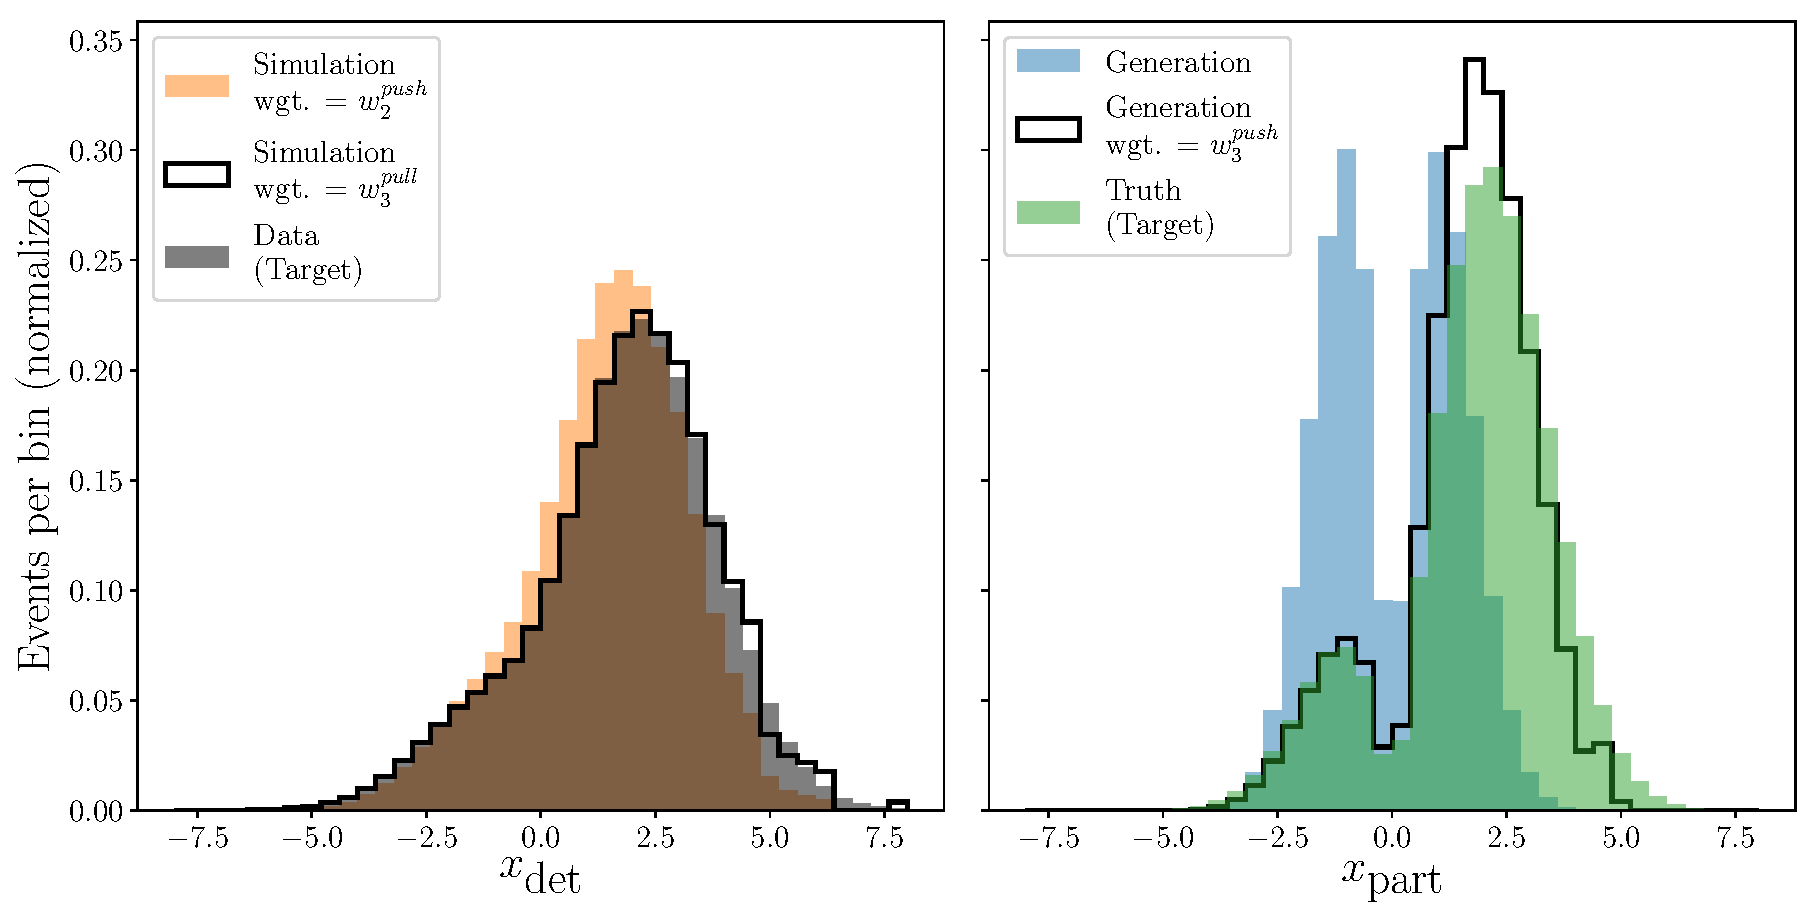
\includegraphics[width=0.45\textwidth]{Figures/GaussianToyExample/GaussianToyExample-MCUnfoldingResultsIteration03.pdf}}\subfloat[4 iterations]{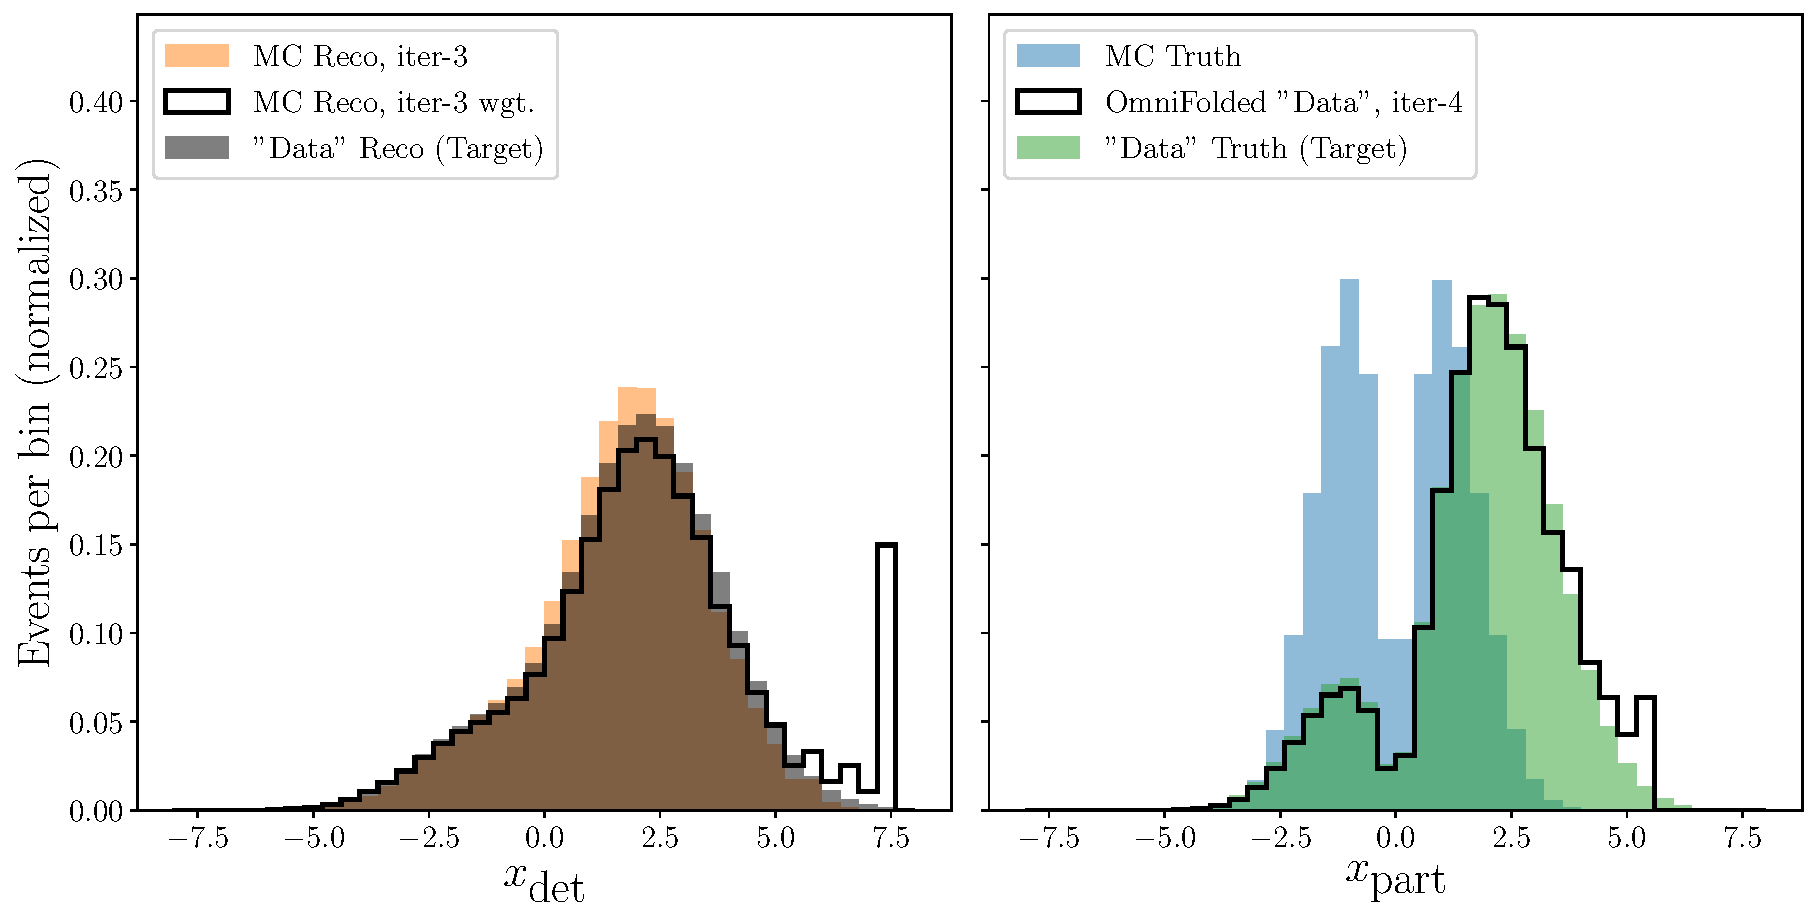
\includegraphics[width=0.45\textwidth]{Figures/GaussianToyExample/GaussianToyExample-MCUnfoldingResultsIteration04.pdf}}\\
\subfloat[5 iterations]{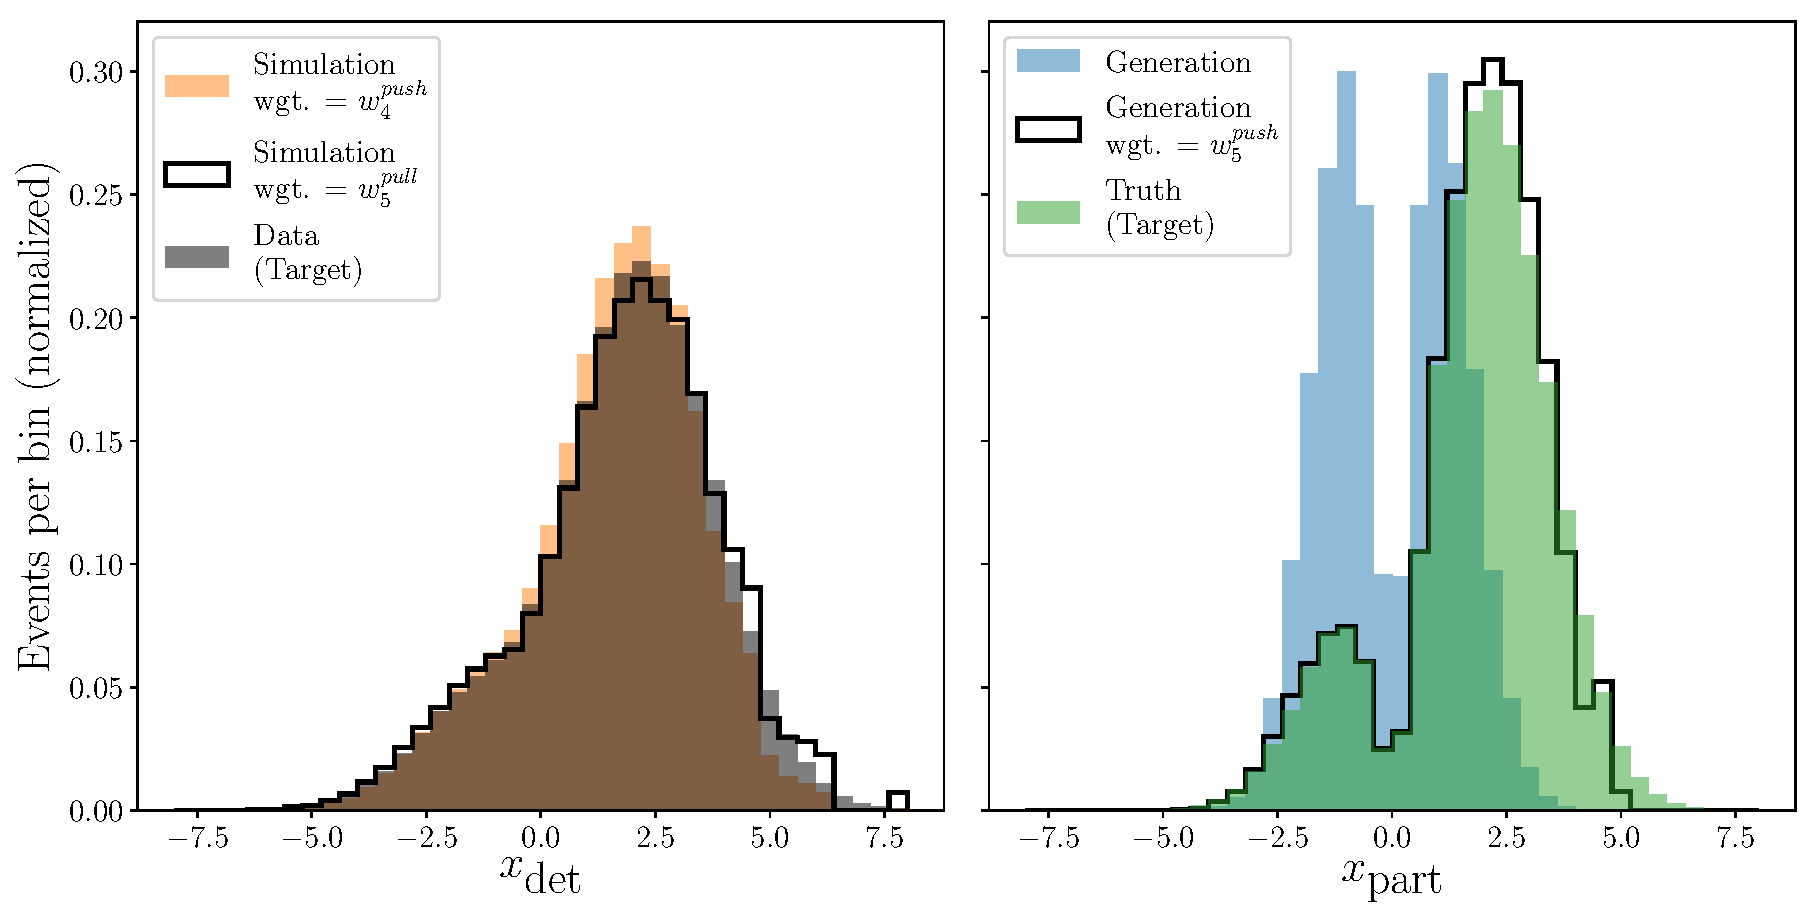
\includegraphics[width=0.45\textwidth]{Figures/GaussianToyExample/GaussianToyExample-MCUnfoldingResultsIteration05.pdf}}\subfloat[6 iterations]{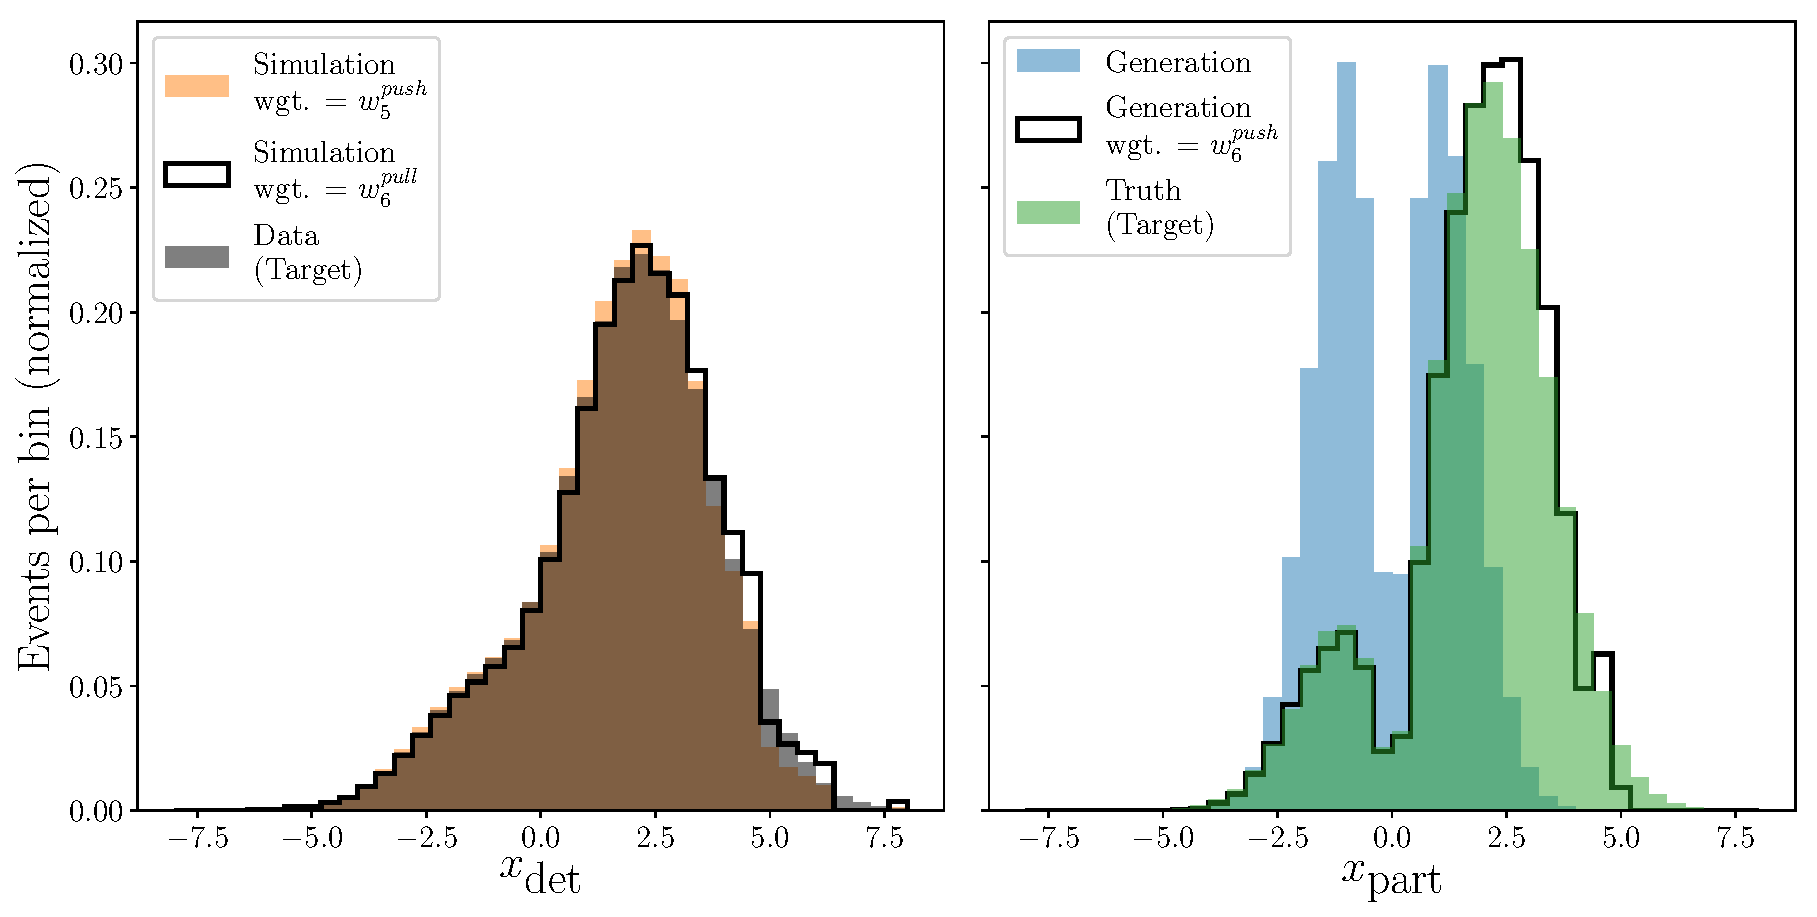
\includegraphics[width=0.45\textwidth]{Figures/GaussianToyExample/GaussianToyExample-MCUnfoldingResultsIteration06.pdf}}
\caption{An illustration of six iterations of the OmniFold algorithm to the one-dimensional Gaussian example with initial MC event weights injected.  For each iteration, the left plot is the detector-level distribution with weights $\omega_n$ and the right plot is the particle-level distribution with weights $\nu_n$.}
\label{fig:gaussian:MCiterations}
\end{figure}

\clearpage

\clearpage

\section{Systematic uncertainties}
\label{sec:uncerts}

Uncertainties on the unfolded result are evaluated using error propagation, consistent with the standard approach used at ATLAS.
Uncertainties are split into sources (sometimes called ``uncertainty components'') that are each treated as uncorrelated to each other.
For each such uncertainty source, a perturbation is introduced either to the MC or data corresponding to its impact: $+1\sigma$, and in case of two-sided uncertainties, also $-1\,\sigma$. The unfolding (``full analysis'') is then repeated using the modified samples, which results in a OmniFold weight $\nu'$ for each event that is slightly different from the nominal OmniFold weight $\nu$. Each event in the unfolded dataset is hence assigned one nominal weight and a list of alternative weights, each corresponding to a systematic uncertainty source, or statistical replica variation.

\subsection{Data and Monte Carlo statistical uncertainties}
These uncertainties will be computed via bootstrapping.  A set of $N$ pseudodatasets are constructed where each event has a weight $W_\text{pseudo}\,w_\text{nominal}$, where $w_\text{nominal}$ is unity for data and $w_\text{MC}$ for simulation. $W_\text{pseudo}$ is a value sampled randomly from a Poisson distribution with a mean of unity.  To ensure that the ``uncertainty on the uncertainty'' is negligible an ensemble of $N\gtrsim 100$ such pseudodatasets can be used.  These uncertainties are straightforward to compute, but are computationally expensive and thus we will compute them once all other results are finished.

\subsection{Pileup reweighting uncertainties}
As discussed in section~\ref{subsec:PRW}, a correction is applied to MC events such that the pileup modeling in the simulation corresponds to what is seen in data. As such, there are variations associated with this modeling
that must be taken into account.

In addition, a scaling correction is applied to the data during pileup reweighting. Nominally, this scaling correction is equal to 1/1.03, and the up and down variations are set to 1/1.072 and 1/1.35 respectively.

Figure~\ref{fig:PRWpTll} shows the effect of these variations for the dilepton \pt across all years.

\begin{figure}[h!]
  \centering
  \subfloat[MC16a]{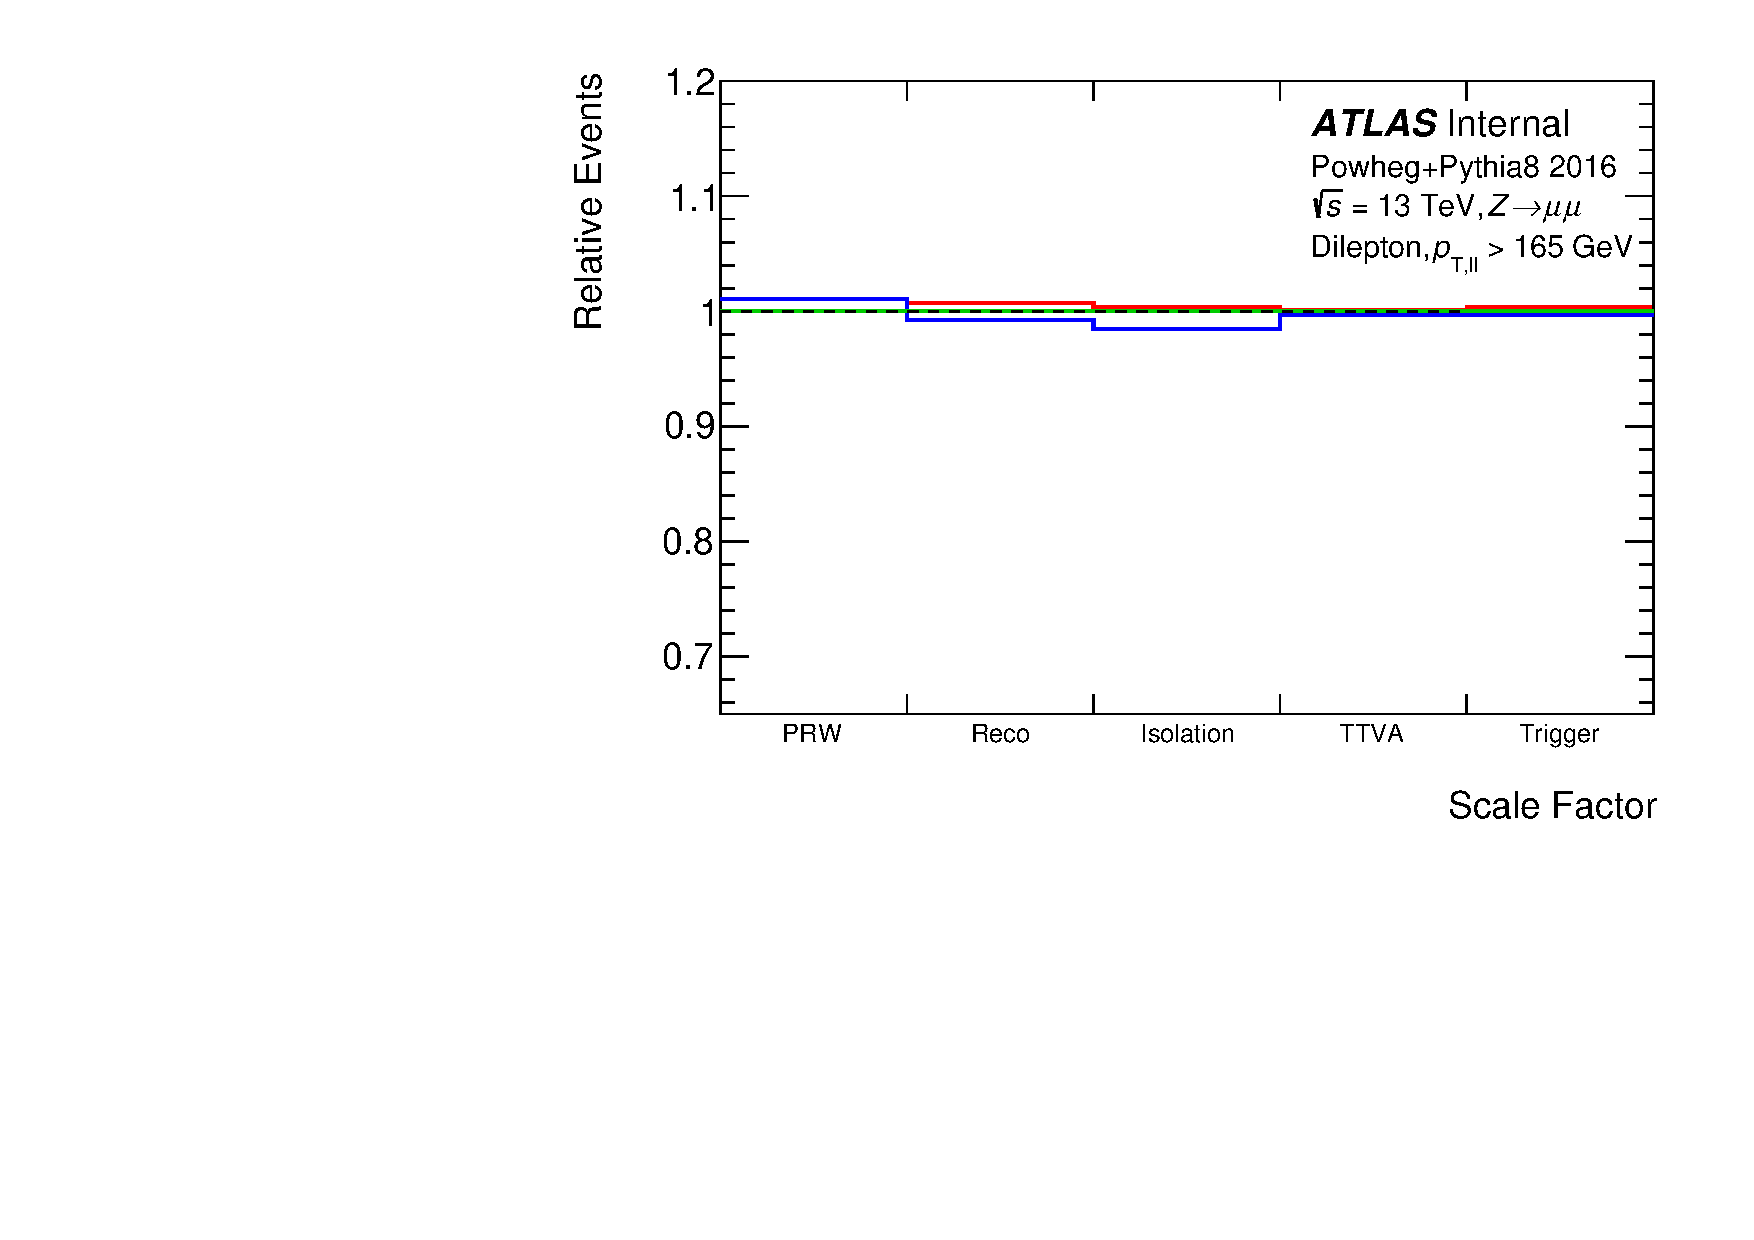
\includegraphics[page=1,width=0.45\textwidth]{figures/ZjetOmnifoldSystematics.pdf}}
  \subfloat[MC16d]{\includegraphics[page=103,width=0.45\textwidth]{figures/ZjetOmnifoldSystematics.pdf}} \\
  \subfloat[MC16e]{\includegraphics[page=205,width=0.45\textwidth]{figures/ZjetOmnifoldSystematics.pdf}}
  \subfloat[Run 2]{\includegraphics[page=307,width=0.45\textwidth]{figures/ZjetOmnifoldSystematics.pdf}}
  \caption{The fractional systematic impact of the up and down variations of the pileup reweighting across all years for the \powheg+\pythia~sample.}
  \label{fig:PRWpTll}
\end{figure}

\subsection{Muon uncertainties}
\label{sec:muonuncerts}

\subsubsection{Muon efficiency uncertainties}
As summarized in section~\ref{subsec:MCCorr} there are several scale factors associated with muon reconstruction related to efficiencies in the trigger, reconstruction, isolation and track-to-vertex association.
Hence, there are 2 systematic variations associated with the trigger efficiency, 2 for the isolation efficiency, 4 for the reconstruction efficiency, and 2 for the TTVA efficiency:
\begin{itemize}
  \setlength{\itemsep}{1pt}\setlength{\parskip}{0pt}\setlength{\parsep}{0pt}
  \item MUON\_EFF\_TrigSystUncertainty
  \item MUON\_EFF\_TrigStatUncertainty
  \item MUON\_EFF\_ISO\_SYS
  \item MUON\_EFF\_ISO\_STAT
  \item MUON\_EFF\_RECO\_SYS
  \item MUON\_EFF\_RECO\_SYS\_LOWPT
  \item MUON\_EFF\_RECO\_STAT
  \item MUON\_EFF\_RECO\_STAT\_LOWPT
  \item MUON\_EFF\_TTVA\_SYS
  \item MUON\_EFF\_TTVA\_STAT
\end{itemize}

The impact of the efficiency systematics is summarized in figure~\ref{fig:PP8SFSyst}.

\begin{figure}[h!]
  \centering
  \subfloat[MC16a]{\includegraphics[page=2,width=0.45\textwidth]{figures/ZjetOmnifoldSystematics.pdf}}
  \subfloat[MC16d]{\includegraphics[page=104,width=0.45\textwidth]{figures/ZjetOmnifoldSystematics.pdf}} \\
  \subfloat[MC16e]{\includegraphics[page=206,width=0.45\textwidth]{figures/ZjetOmnifoldSystematics.pdf}}
  \subfloat[Run 2]{\includegraphics[page=308,width=0.45\textwidth]{figures/ZjetOmnifoldSystematics.pdf}}
  \caption{The fractional systematic impact for the muon efficiencies for the \powheg+\pythia~samples across all years as a function of the dilepton \pt.}
  \label{fig:PP8SFSyst}
\end{figure}

\subsubsection{Muon calibration uncertainties}
There are also systematic variations associated with the calibration applied to the muons. These will have an affect on the muon kinematics. The systematic variations are listed below, and include
one for momentum variations due to measurements made in the inner detector, one for momentum effects related to the muon spectrometer, one for the momentum scale, and 2 systematics related to the measured sagitta value.
\begin{itemize}
  \setlength{\itemsep}{1pt}\setlength{\parskip}{0pt}\setlength{\parsep}{0pt}
  \item MUON\_ID (inner detector track resolution)
  \item MUON\_MS (muon spectrometer track resolution)
  \item MUON\_SCALE (momentum scale)
  \item MUON\_SAGITTA\_RESBIAS (residual bias correction)
  \item MUON\_SAGITTA\_RHO (combined measurement correction)
\end{itemize}

The effects of these variations on the dilepton \pt and mass are shown in figure~\ref{fig:PP8MuCalSystpTll} and~\ref{fig:PP8MuCalSystmll}.

\begin{figure}[h!]
  \centering
  \subfloat[MC16a]{\includegraphics[page=97,width=\textwidth]{figures/ZjetOmnifoldSystematics.pdf}} \\
  \subfloat[MC16d]{\includegraphics[page=199,width=\textwidth]{figures/ZjetOmnifoldSystematics.pdf}} \\
  \subfloat[MC16e]{\includegraphics[page=301,width=\textwidth]{figures/ZjetOmnifoldSystematics.pdf}} \\
  \subfloat[Run 2]{\includegraphics[page=403,width=\textwidth]{figures/ZjetOmnifoldSystematics.pdf}}
  \caption{The fractional systematic impact for variations to the muon calibration for the \powheg+\pythia~samples for all years as a function of the dilepton \pt. The upwards shift is presented in red, and the downwards shift in blue.}
  \label{fig:PP8MuCalSystpTll}
\end{figure}

\begin{figure}[h!]
  \centering
  \subfloat[MC16a]{\includegraphics[page=99,width=\textwidth]{figures/ZjetOmnifoldSystematics.pdf}} \\
  \subfloat[MC16d]{\includegraphics[page=201,width=\textwidth]{figures/ZjetOmnifoldSystematics.pdf}} \\
  \subfloat[MC16e]{\includegraphics[page=303,width=\textwidth]{figures/ZjetOmnifoldSystematics.pdf}} \\
  \subfloat[Run 2]{\includegraphics[page=405,width=\textwidth]{figures/ZjetOmnifoldSystematics.pdf}}
  \caption{The fractional systematic impact for variations to the muon calibration for the \powheg+\pythia~samples for all years as a function of the dilepton mass. The upwards shift is presented in red, and the downwards shift in blue.}
  \label{fig:PP8MuCalSystmll}
\end{figure}

\subsection{Track uncertainties}

The systematic uncertainties associated with the tracks are:

\begin{itemize}
  \setlength{\itemsep}{1pt}\setlength{\parskip}{0pt}\setlength{\parsep}{0pt}
  \item InDet::TRK\_EFF\_TIGHT\_GLOBAL
  \item InDet::TRK\_EFF\_TIGHT\_IBL
  \item InDet::TRK\_EFF\_TIGHT\_PP0
  \item InDet::TRK\_EFF\_TIGHT\_PHYSMODEL
  \item InDet::TRK\_EFF\_LOOSE\_TIDE
  \item InDet::TRK\_FAKE\_RATE\_LOOSE
  \item InDet::TRK\_BIAS\_QOVERP\_SAGITTA\_WM
\end{itemize}

The first four are combined into one nuisance parameter and are due to variations of the tracking efficiency. The fifth describes the variations to the tracking efficiency when the track is inside a jet.
The sixth represents variations to the fake rate. The last varies the \pt of the track based on the residual alignment uncertainties. Figure~\ref{fig:PP8TrackSyst} shows the effect of these variations on the \pt of the tracks in the \powheg+\pythia~sample across all years.

\begin{figure}[h!]
  \centering
  \subfloat[MC16a]{\includegraphics[page=102,width=0.45\textwidth]{figures/ZjetOmnifoldSystematics.pdf}}
  \subfloat[MC16d]{\includegraphics[page=204,width=0.45\textwidth]{figures/ZjetOmnifoldSystematics.pdf}} \\
  \subfloat[MC16e]{\includegraphics[page=306,width=0.45\textwidth]{figures/ZjetOmnifoldSystematics.pdf}}
  \subfloat[Run 2]{\includegraphics[page=408,width=0.45\textwidth]{figures/ZjetOmnifoldSystematics.pdf}}
  \caption{The fractional systematic impact for variations applied to the tracks for the \powheg+\pythia~samples for all years. Note that only the down variations are shown for the inclusive efficiency, inside jet efficiency and the fake rate.
  The variations are symmetrized for use in the analysis.}
  \label{fig:PP8TrackSyst}
\end{figure}

The track systematics will also have an effect on the track jet observables. Figure~\ref{fig:PP8TrackJetSyst} shows the fractional effect of the track systematics on the \pt, $y$, $m$, $\tau_1$, and the number of constituents of the leading track jet.

\begin{figure}[h!]
  \centering
  \subfloat{\includegraphics[page=332,width=0.45\textwidth]{figures/ZjetOmnifoldSystematics.pdf}}
  \subfloat{\includegraphics[page=335,width=0.45\textwidth]{figures/ZjetOmnifoldSystematics.pdf}} \\
  \subfloat{\includegraphics[page=341,width=0.45\textwidth]{figures/ZjetOmnifoldSystematics.pdf}}
  \subfloat{\includegraphics[page=344,width=0.45\textwidth]{figures/ZjetOmnifoldSystematics.pdf}} \\
  \subfloat{\includegraphics[page=374,width=0.45\textwidth]{figures/ZjetOmnifoldSystematics.pdf}}
  \caption{The fractional systematic impact of the track variations on various track jet observables for the full Run 2 dataset of the \powheg+\pythia~sample.}
  \label{fig:PP8TrackJetSyst}
\end{figure}

\subsection{Modeling and unfolding uncertainties}

Modeling uncertainties are determined by unfolding the data with simulations that have different physics models.  We will do this by first comparing the result when unfolding with \pythia{} and when unfolding with \sherpa.  This is a crude uncertainty because there are multiple differences between these generators.  We will complement this comparison by unfolding with various \powheg+\pythia{} samples (see Sec.~\ref{sec:theoryuncerts}) that have been re-weighted based on truth-level samples that have targeted variations (e.g.\ A14 tune variations).  Additional samples are being prepared by the PMG but will likely not be ready in time for this analysis.

Unfolding uncertainties are designed to quantify the method closure.  We will do this by unfolding \pythia{} with \sherpa{} and then comparing to the \pythia{} truth (and vice versa).  This may have some double-counting with modeling uncertainties and is often mitigated by performing some reweighting\footnote{\url{https://twiki.cern.ch/twiki/bin/viewauth/AtlasProtected/StandardModelUnfolding}}~\cite{Malaescu:2009dm} (which actually is similar to OmniFold Step 1).  However, we will choose the more conservative approach for this first high-dimensional analysis.

\clearpage

\subsection{Theoretical uncertainties}
\label{sec:theoryuncerts}
\subsubsection{QCD renormalization and factorization scale variations}
The variation of the QCD renormalization ($\mu_r$) and factorization ($\mu_f$) scale on the process was studied using the \sherpa\ event generator (one of our nominal samples).
This sample contains event weights corresponding to the standard variations of $\times 2$ and $\times 0.5$ for each scale.
%This generator can vary each scale independently and provides combinations of up (2$\mu_(r,f)$) and down (0.5$\mu_(r,f)$) variations of each scale.
The impact of each variation relative to the nominal scale choice is shown in figure~\ref{fig:QCDscale_mjj}.
Both $\mu_r$ and $\mu_f$ varied up is denoted ``uu'' and both varied down ``dd'', while ``n" indicates the nominal quantity etc.
A larger renormalization scales results in a smaller cross section and hence less events in the observed dilepton \pt spectrum, and vice versa.
Varying the factorization scale has very little impact.

\begin{figure}[h!]
  \centering
  \subfloat[MC16a]{\includegraphics[page=2,width=0.45\textwidth]{figures/systQCD.pdf}}
  \subfloat[MC16d]{\includegraphics[page=4,width=0.45\textwidth]{figures/systQCD.pdf}} \\
  \subfloat[MC16e]{\includegraphics[page=6,width=0.45\textwidth]{figures/systQCD.pdf}}
  \subfloat[Run 2]{\includegraphics[page=7,width=0.45\textwidth]{figures/systQCD.pdf}}
  \caption{The fractional impact of the QCD scale variations for the \sherpa~samples on the dilepton \pt spectrum for all the years and full Run2. The result of varying $\mu_r$ and $\mu_f$ in the up direction is shown in dark red and the downwards shift is in dark blue color. The lighter blue and red show the result of only varying $\mu_r$, and the green lines only varying $\mu_f$.}
  \label{fig:QCDscale_mjj}
\end{figure}

\subsubsection{Parton Shower (PS) uncertainties}
To compute uncertainty for PS, the \powheg$+$\pythia~sample with AZNLO tune are used [listed in~\ref{app:datasets}]. A set of systematic variations is provided for the AZNLO tune, based on the eigentune method. In order to cover the full range of PS uncertainties, a subset of tune variations which together provide maximal coverage of the observables: one pair mainly for underlying event effects (Var1), one pair mainly for jet structure effects (Var2), along with scale variations (RenUp and RenDown) and MultipartonInteractions (MPI) variations (MPIUp and MPIDown) is used. The impact of these variation relative to the nominal sample is shown in figure~\ref{fig:PS_MPI}.

\begin{figure}[h!]
  \centering
  \subfloat[]{\includegraphics[page=1,width=0.45\textwidth]{figures/ShowerVartions_pTll.pdf}}
  \subfloat[]{\includegraphics[page=1,width=0.45\textwidth]{figures/ShowerVartions_Ntracks.pdf}} \\
  \subfloat[]{\includegraphics[page=2,width=0.45\textwidth]{figures/ShowerVartions_Ntracks.pdf}}
  \subfloat[]{\includegraphics[page=3,width=0.45\textwidth]{figures/ShowerVartions_Ntracks.pdf}}\\
  \subfloat[]{\includegraphics[page=4,width=0.45\textwidth]{figures/ShowerVartions_Ntracks.pdf}}
  \subfloat[]{\includegraphics[page=2,width=0.45\textwidth]{figures/ShowerVartions_etaTracks.pdf}}
  \caption{The fractional impact of the MC tuning and MPI variations for the \pythia~samples on the track jet properties and dilepton \pt for full Run2. Systematic effect evaluated by varying different parameters of the MC samples. The statistical uncertainties on these uncertainties are about 0.001\%, 0.05\% and 3\% in the three bins.}
  \label{fig:PS_MPI}
\end{figure}

\subsubsection{Parton Distribution Function (PDF) variations}
The variability of the underlying PDF is calculated using the \sherpa~samples. The nominal PDF used by the generator is the central value of some underlying PDF distribution, the \sherpa~generator provides 100 variations to this nominal pdf that are generated from this underlying statistical distribution.  The RMS of these 100 results is interpreted as a systematic uncertainty, this spread is shown for the measurement in figure~\ref{fig:PDF_RMS}. Also the fractional impact of the $\alpha_{s}$ variations and two alternative PDF sets is shown in figure~\ref{fig:alpha_S}.
\begin{figure}[h!]
  \centering
  \subfloat[]{\includegraphics[page=1,width=0.45\textwidth]{figures/systPDF_100.pdf}}
  \subfloat[]{\includegraphics[page=1,width=0.45\textwidth]{figures/systPDF_RMS.pdf}} \\
  \caption{Spread of 100 PDF variations per bin (left) and impact of systematic uncertainty as RMS of these 100 results (right) on dilepton \pt. To show smooth variations in these plots, some events with large negative weights are skipped.}
  \label{fig:PDF_RMS}
\end{figure}

\begin{figure}[h!]
  \centering
  \includegraphics[page=2,width=0.45\textwidth]{figures/syst_alphaS.pdf} \\
  \caption{The fractional impact of the $\alpha_{s}$ variations for the \sherpa~samples on the dilepton \pt spectrum. The result of varying $\alpha_{s}$ in the up direction is shown in dark red and the downwards shift is in dark blue color. The lighter green and black color show uncertainty for the two alternative PDF sets.}
  \label{fig:alpha_S}
\end{figure}


%-------------------------------------------------------------------------------
\section{Results}
\label{sec:result}
\subsection{Blinding strategy}

We have investigated data/MC differences at detector-level, but we remain blinded to the unfolded data until following the Editorial Board's approval of the procedure.

\subsection{Proposed presentation of results}

Unlike all other ATLAS measurements to date, the results here are \textbf{unbinned}.
Starting from the unbinned results, it is trivial to create histograms with any binning, which is convenient for presentation and comparison with binned measurments performed using traditional techniques.
The proposed main results to be included in the first paper is:

%Clearly, we can represent the data as histograms, but that is restrictive.

\begin{itemize}
\item
  Unbinned simultaneous unfolding of a set of 24 observables using the MultiFold technique.
  The observables are:
  \begin{itemize}
    \item
      the transverse momentum \ptll{} and rapidity $\yll$ of the dimuon system, which probes the $Z$-boson kinematics;
    \item
      the transverse momentum (\ptlm, \ptsm),
      %OR ($p_{\mathrm{T},\mu 1}$, $p_{\mathrm{T},\mu 2}$)
      rapidity (\ylm{}, \ysm) and azimuthal angle (\philm, \phism) of the two muons probing the $Z$-boson decay kinematics;
    \item
      the transverse momentum (\ptlj, \ptsj), rapidity (\ylj{}, \ysj), azimuth (\philj, \phisj) of the two highest-\pt{} charged hadron jets in the event, which probes the jet kinematics; and
    \item
      the mass (\mlj, \msj), charged hadron multiplicity (\Nclj, \Ncsj) and $N$-subjettiness quantities \taulj{1}, %$\tau_1(j1)$, $\tau_{1,\mathrm{j1}}$ 
      \tausj{1}, \taulj{2}, \tausj{2}, \taulj{3} and \tausj{3} that measures the substructure of the leading two charged-hadron jets. 
  \end{itemize}  
\item
   A plot will be produced for each observable comparing the unfolded spectrum with a measurement performed using IBU (i.e.\ the standard technique used in ATLAS SM measurements).
   IBU requires a predefined binning, which has been derived for each observable as described in appendix~\ref{app:IBU}. This binning is presented in table~\ref{tab:IBUBins}.
%Our paper will contain a small number of unfolded histograms to illustrate the breadth of the result.
%We will show plots that show the spectra of the multifold observables, using IBU, MultiFold, and OmniFold in the support note (and also include the correlation dimension~\cite{Komiske:2019fks}) and then we will discuss with the Editorial Board which plots to go in the paper.
\item
  \todo{This is only for OmniFold, right? We'd need to make a flat n-tuple with 24 branches, I think, which should be stated here}
  We make public the weight function(s) (as a neural network, saving the model architecture and weights from TensorFlow) and the exact configuration used to generate the nominal MC events.  There will be one function per systematic uncertainty.  This, combined with a Rivet routine of the analysis selection, will ensure that the data can be used and readily and widely reinterpreted.
\item (Alternative: we make public our simulated MC sample with a vector of weights for each event)
\end{itemize}


For a second, future paper, the idea is to include...


%-------------------------------------------------------------------------------
\section{Conclusion}
\label{sec:conclusion}
%-------------------------------------------------------------------------------

\textit{To be filled in once we have unblinded.}


%-------------------------------------------------------------------------------
% If you use biblatex and either biber or bibtex to process the bibliography
% just say \printbibliography here
\printbibliography
% If you want to use the traditional BibTeX you need to use the syntax below.
%\bibliographystyle{bib/bst/atlasBibStyleWithTitle}
%\bibliography{ANA-STDM-2020-17-INT1,bib/ATLAS,bib/CMS,bib/ConfNotes,bib/PubNotes}
%-------------------------------------------------------------------------------

%-------------------------------------------------------------------------------
% Print the list of contributors to the analysis
% The argument gives the fraction of the text width used for the names
%-------------------------------------------------------------------------------
\clearpage
%The supporting notes for the analysis should also contain a list of contributors.
%This information should usually be included in \texttt{mydocument-metadata.tex}.
%The list should be printed either here or before the Table of Contents.
%\PrintAtlasContribute{0.30}


%-------------------------------------------------------------------------------
\clearpage
\appendix
\part*{Appendices}
\addcontentsline{toc}{part}{Appendices}
%-------------------------------------------------------------------------------

%% Appendix A
\section{Software}

We use the STDM7 derivation\footnote{\url{https://gitlab.cern.ch/atlas/athena/-/blob/master/PhysicsAnalysis/DerivationFramework/DerivationFrameworkSM/share/STDM7.py}} from the Standard Model group because it stores all of the tracks in events and has a dilepton requirement. 

The event selection software can be found at \url{https://gitlab.cern.ch/carleton-ATLAS/omnifold-analysis} and the unfolding software can be found at \url{https://github.com/bnachman/ATLASOmniFold}.  Both of these are currently private repositories, since they are not hosted on CERN's Gitlab, but we are happy to add anyone who would like to see them.  The reason for this setup is that we have non-ATLAS author collaborators.  

%% Appendix B
\section{Data and Monte Carlo samples}
\label{app:datasets}

\subsection{Data}
\begin{tiny}
\begin{verbatim}
data15_13TeV.periodD.physics_Main.PhysCont.DAOD_STDM7.grp23_v01_4397
data15_13TeV.periodE.physics_Main.PhysCont.DAOD_STDM7.grp23_v01_4397
data15_13TeV.periodF.physics_Main.PhysCont.DAOD_STDM7.grp23_v01_4397
data15_13TeV.periodG.physics_Main.PhysCont.DAOD_STDM7.grp23_v01_4397
data15_13TeV.periodH.physics_Main.PhysCont.DAOD_STDM7.grp23_v01_4397
data15_13TeV.periodJ.physics_Main.PhysCont.DAOD_STDM7.grp23_v01_4397

data16_13TeV.periodA.physics_Main.PhysCont.DAOD_STDM7.grp23_v01_4397
data16_13TeV.periodB.physics_Main.PhysCont.DAOD_STDM7.grp23_v01_4397
data16_13TeV.periodC.physics_Main.PhysCont.DAOD_STDM7.grp23_v01_4397
data16_13TeV.periodD.physics_Main.PhysCont.DAOD_STDM7.grp23_v01_4397
data16_13TeV.periodE.physics_Main.PhysCont.DAOD_STDM7.grp23_v01_4397
data16_13TeV.periodF.physics_Main.PhysCont.DAOD_STDM7.grp23_v01_4397
data16_13TeV.periodG.physics_Main.PhysCont.DAOD_STDM7.grp23_v01_4397
data16_13TeV.periodI.physics_Main.PhysCont.DAOD_STDM7.grp23_v01_4397
data16_13TeV.periodK.physics_Main.PhysCont.DAOD_STDM7.grp23_v01_4397
data16_13TeV.periodL.physics_Main.PhysCont.DAOD_STDM7.grp23_v01_4397

data17_13TeV.periodB.physics_Main.PhysCont.DAOD_STDM7.grp23_v01_p4397
data17_13TeV.periodC.physics_Main.PhysCont.DAOD_STDM7.grp23_v01_p4397
data17_13TeV.periodD.physics_Main.PhysCont.DAOD_STDM7.grp23_v01_p4397
data17_13TeV.periodE.physics_Main.PhysCont.DAOD_STDM7.grp23_v01_p4397
data17_13TeV.periodF.physics_Main.PhysCont.DAOD_STDM7.grp23_v01_p4397
data17_13TeV.periodH.physics_Main.PhysCont.DAOD_STDM7.grp23_v01_p4397
data17_13TeV.periodI.physics_Main.PhysCont.DAOD_STDM7.grp23_v01_p4397
data17_13TeV.periodK.physics_Main.PhysCont.DAOD_STDM7.grp23_v01_p4397

data18_13TeV.periodB.physics_Main.PhysCont.DAOD_STDM7.grp23_v01_p4397
data18_13TeV.periodC.physics_Main.PhysCont.DAOD_STDM7.grp23_v01_p4397
data18_13TeV.periodD.physics_Main.PhysCont.DAOD_STDM7.grp23_v01_p4397
data18_13TeV.periodF.physics_Main.PhysCont.DAOD_STDM7.grp23_v01_p4397
data18_13TeV.periodI.physics_Main.PhysCont.DAOD_STDM7.grp23_v01_p4397
data18_13TeV.periodK.physics_Main.PhysCont.DAOD_STDM7.grp23_v01_p4397
data18_13TeV.periodL.physics_Main.PhysCont.DAOD_STDM7.grp23_v01_p4397
data18_13TeV.periodM.physics_Main.PhysCont.DAOD_STDM7.grp23_v01_p4397
data18_13TeV.periodO.physics_Main.PhysCont.DAOD_STDM7.grp23_v01_p4397
data18_13TeV.periodQ.physics_Main.PhysCont.DAOD_STDM7.grp23_v01_p4397

\end{verbatim}
\end{tiny}

\subsection{Monte Carlo}

\subsubsection{Powheg+Pythia8 samples}

\begin{tiny}
\begin{verbatim}
mc16_13TeV.361107.PowhegPythia8EvtGen_AZNLOCTEQ6L1_Zmumu.deriv.DAOD_STDM7.e3601_s3126_r9364_p4145
mc16_13TeV.361107.PowhegPythia8EvtGen_AZNLOCTEQ6L1_Zmumu.deriv.DAOD_STDM7.e3601_s3126_r10201_p4145
mc16_13TeV.361107.PowhegPythia8EvtGen_AZNLOCTEQ6L1_Zmumu.deriv.DAOD_STDM7.e3601_s3126_r10724_p4145
\end{verbatim}
\end{tiny}

\subsubsection{Sherpa 2.2.1 samples}

\begin{tiny}
\begin{verbatim}
mc16_13TeV.364100.Sherpa_221_NNPDF30NNLO_Zmumu_MAXHTPTV0_70_CVetoBVeto.deriv.DAOD_STDM7.e5271_s3126_r9364_p4357
mc16_13TeV.364101.Sherpa_221_NNPDF30NNLO_Zmumu_MAXHTPTV0_70_CFilterBVeto.deriv.DAOD_STDM7.e5271_s3126_r9364_p4357
mc16_13TeV.364102.Sherpa_221_NNPDF30NNLO_Zmumu_MAXHTPTV0_70_BFilter.deriv.DAOD_STDM7.e5271_s3126_r9364_p4357
mc16_13TeV.364103.Sherpa_221_NNPDF30NNLO_Zmumu_MAXHTPTV70_140_CVetoBVeto.deriv.DAOD_STDM7.e5271_s3126_r9364_p4357
mc16_13TeV.364104.Sherpa_221_NNPDF30NNLO_Zmumu_MAXHTPTV70_140_CFilterBVeto.deriv.DAOD_STDM7.e5271_s3126_r9364_p4357
mc16_13TeV.364105.Sherpa_221_NNPDF30NNLO_Zmumu_MAXHTPTV70_140_BFilter.deriv.DAOD_STDM7.e5271_s3126_r9364_p4357
mc16_13TeV.364106.Sherpa_221_NNPDF30NNLO_Zmumu_MAXHTPTV140_280_CVetoBVeto.deriv.DAOD_STDM7.e5271_s3126_r9364_p4357
mc16_13TeV.364107.Sherpa_221_NNPDF30NNLO_Zmumu_MAXHTPTV140_280_CFilterBVeto.deriv.DAOD_STDM7.e5271_s3126_r9364_p4357
mc16_13TeV.364108.Sherpa_221_NNPDF30NNLO_Zmumu_MAXHTPTV140_280_BFilter.deriv.DAOD_STDM7.e5271_s3126_r9364_p4357
mc16_13TeV.364109.Sherpa_221_NNPDF30NNLO_Zmumu_MAXHTPTV280_500_CVetoBVeto.deriv.DAOD_STDM7.e5271_s3126_r9364_p4357
mc16_13TeV.364110.Sherpa_221_NNPDF30NNLO_Zmumu_MAXHTPTV280_500_CFilterBVeto.deriv.DAOD_STDM7.e5271_s3126_r9364_p4357
mc16_13TeV.364111.Sherpa_221_NNPDF30NNLO_Zmumu_MAXHTPTV280_500_BFilter.deriv.DAOD_STDM7.e5271_s3126_r9364_p4357
mc16_13TeV.364112.Sherpa_221_NNPDF30NNLO_Zmumu_MAXHTPTV500_1000.deriv.DAOD_STDM7.e5271_s3126_r9364_p4357
mc16_13TeV.364113.Sherpa_221_NNPDF30NNLO_Zmumu_MAXHTPTV1000_E_CMS.deriv.DAOD_STDM7.e5271_s3126_r9364_p4357

mc16_13TeV.364100.Sherpa_221_NNPDF30NNLO_Zmumu_MAXHTPTV0_70_CVetoBVeto.deriv.DAOD_STDM7.e5271_s3126_r10201_p4357
mc16_13TeV.364101.Sherpa_221_NNPDF30NNLO_Zmumu_MAXHTPTV0_70_CFilterBVeto.deriv.DAOD_STDM7.e5271_s3126_r10201_p4357
mc16_13TeV.364102.Sherpa_221_NNPDF30NNLO_Zmumu_MAXHTPTV0_70_BFilter.deriv.DAOD_STDM7.e5271_s3126_r10201_p4357
mc16_13TeV.364103.Sherpa_221_NNPDF30NNLO_Zmumu_MAXHTPTV70_140_CVetoBVeto.deriv.DAOD_STDM7.e5271_s3126_r10201_p4357
mc16_13TeV.364104.Sherpa_221_NNPDF30NNLO_Zmumu_MAXHTPTV70_140_CFilterBVeto.deriv.DAOD_STDM7.e5271_s3126_r10201_p4357
mc16_13TeV.364105.Sherpa_221_NNPDF30NNLO_Zmumu_MAXHTPTV70_140_BFilter.deriv.DAOD_STDM7.e5271_s3126_r10201_p4357
mc16_13TeV.364106.Sherpa_221_NNPDF30NNLO_Zmumu_MAXHTPTV140_280_CVetoBVeto.deriv.DAOD_STDM7.e5271_s3126_r10201_p4357
mc16_13TeV.364107.Sherpa_221_NNPDF30NNLO_Zmumu_MAXHTPTV140_280_CFilterBVeto.deriv.DAOD_STDM7.e5271_s3126_r10201_p4357
mc16_13TeV.364108.Sherpa_221_NNPDF30NNLO_Zmumu_MAXHTPTV140_280_BFilter.deriv.DAOD_STDM7.e5271_s3126_r10201_p4357
mc16_13TeV.364109.Sherpa_221_NNPDF30NNLO_Zmumu_MAXHTPTV280_500_CVetoBVeto.deriv.DAOD_STDM7.e5271_s3126_r10201_p4357
mc16_13TeV.364110.Sherpa_221_NNPDF30NNLO_Zmumu_MAXHTPTV280_500_CFilterBVeto.deriv.DAOD_STDM7.e5271_s3126_r10201_p4357
mc16_13TeV.364111.Sherpa_221_NNPDF30NNLO_Zmumu_MAXHTPTV280_500_BFilter.deriv.DAOD_STDM7.e5271_s3126_r10201_p4357
mc16_13TeV.364112.Sherpa_221_NNPDF30NNLO_Zmumu_MAXHTPTV500_1000.deriv.DAOD_STDM7.e5271_s3126_r10201_p4357
mc16_13TeV.364113.Sherpa_221_NNPDF30NNLO_Zmumu_MAXHTPTV1000_E_CMS.deriv.DAOD_STDM7.e5271_s3126_r10201_p4357

mc16_13TeV.364100.Sherpa_221_NNPDF30NNLO_Zmumu_MAXHTPTV0_70_CVetoBVeto.deriv.DAOD_STDM7.e5271_s3126_r10724_p4357
mc16_13TeV.364101.Sherpa_221_NNPDF30NNLO_Zmumu_MAXHTPTV0_70_CFilterBVeto.deriv.DAOD_STDM7.e5271_s3126_r10724_p4357
mc16_13TeV.364102.Sherpa_221_NNPDF30NNLO_Zmumu_MAXHTPTV0_70_BFilter.deriv.DAOD_STDM7.e5271_s3126_r10724_p4357
mc16_13TeV.364103.Sherpa_221_NNPDF30NNLO_Zmumu_MAXHTPTV70_140_CVetoBVeto.deriv.DAOD_STDM7.e5271_s3126_r10724_p4357
mc16_13TeV.364104.Sherpa_221_NNPDF30NNLO_Zmumu_MAXHTPTV70_140_CFilterBVeto.deriv.DAOD_STDM7.e5271_s3126_r10724_p4357
mc16_13TeV.364105.Sherpa_221_NNPDF30NNLO_Zmumu_MAXHTPTV70_140_BFilter.deriv.DAOD_STDM7.e5271_s3126_r10724_p4357
mc16_13TeV.364106.Sherpa_221_NNPDF30NNLO_Zmumu_MAXHTPTV140_280_CVetoBVeto.deriv.DAOD_STDM7.e5271_s3126_r10724_p4357
mc16_13TeV.364107.Sherpa_221_NNPDF30NNLO_Zmumu_MAXHTPTV140_280_CFilterBVeto.deriv.DAOD_STDM7.e5271_s3126_r10724_p4357
mc16_13TeV.364108.Sherpa_221_NNPDF30NNLO_Zmumu_MAXHTPTV140_280_BFilter.deriv.DAOD_STDM7.e5271_s3126_r10724_p4357
mc16_13TeV.364109.Sherpa_221_NNPDF30NNLO_Zmumu_MAXHTPTV280_500_CVetoBVeto.deriv.DAOD_STDM7.e5271_s3126_r10724_p4357
mc16_13TeV.364110.Sherpa_221_NNPDF30NNLO_Zmumu_MAXHTPTV280_500_CFilterBVeto.deriv.DAOD_STDM7.e5271_s3126_r10724_p4357
mc16_13TeV.364111.Sherpa_221_NNPDF30NNLO_Zmumu_MAXHTPTV280_500_BFilter.deriv.DAOD_STDM7.e5271_s3126_r10724_p4357
mc16_13TeV.364112.Sherpa_221_NNPDF30NNLO_Zmumu_MAXHTPTV500_1000.deriv.DAOD_STDM7.e5271_s3126_r10724_p4357
mc16_13TeV.364113.Sherpa_221_NNPDF30NNLO_Zmumu_MAXHTPTV1000_E_CMS.deriv.DAOD_STDM7.e5271_s3126_r10724_p4357
\end{verbatim}
\end{tiny}


%% Appendix C
\section{Particle composition and detector response of hadronic recoil}

This section examines the particle composition and the detector response of the leading jet that balance the $Z$~boson in the fiducial region of the analysis.
The Powheg $Z\to \mu\mu$ sample is used. The particle origin of each track is obtained using the \texttt{truthParticleLink} to find the truth identification of each reconstructed track (see section~\ref{sec:samples}). In addition to the standard event preselection described in section~\ref{sec:selection}, extra cuts are used to make sure the leading reconstructed jet matches the leading particle jet in each event.
%To ensure the closet matching between the leading reconstructed jet and leading truth jet, and always have very good DR between them, the cut on ratio of
This is achieved by requiring $|y_\mathrm{j1}|<2.1$ and $\pTlj / \pTsj < 0.7$. The selection is applied on reconstructed level. However, due to the additional criterion, the leading particle-level (truth) jet will always match the leading reco jet. Note that the jets will have a very high \pt{} since the event selection includes the selection $\pTll > \SI{165}{\GeV}$, and the jet will have a similar \pt{} to that of the $Z$~boson. 

Further events are required to pass track-to-vertex association (TTVA) recommendations as described in section~\ref{subsubsec:trigger}. There are three recommending working points for \texttt{TTVA}, however studies have been done for two only i.e \texttt{loose} and \texttt{tight TTVA} selection.  

Particles are classified depending to their type in the following categories: \texttt{pion} for $\pi^+$ and $\pi^-$; \texttt{kaon} for charged kaons; \texttt{proton};
\texttt{mu} for $\mu^-$ or $\mu^+$; \texttt{e} for $e^-$ or $e^+$;
strange for any charge hadron with strange content other than kaons; \texttt{neutral} for any neutral hadron; \texttt{gam} for photons. As mentioned above, tracks are classified in the same categories using the \texttt{truthParticleLink}. In case there is no truth particle match, it is labelled unmatched. This includes contributions from pileup particles and fake tracks (and possibly secondaries).

All of the reconstructed tracks inside leading jet as well as charged-particles in the associated particle-level jets that are not matched to reconstructed tracks are used for the plots shown in this section. 

Figures~\ref{fig:r_pion_kaon} to ~\ref{fig:r_trackjet} are showing the detector response for each particle category for tight and loose TTVA working point. The pion and kaon response for \texttt{loose} and \texttt{tight TTVA} is ~94\% and ~93\% respectively.

Figure~\ref{fig:frac_unmatchedtracks} depicts fraction of unmatched track w.r.t reco level jet, which indicates ~3\% and ~8\% unmatched tracks for \texttt{tight} and \texttt{loose TTVA} working point respectively. Since \texttt{tight TTVA}  selection reduces ~5\% unmatched tracks as compare to \texttt{loose TTVA}, therefore for the current analysis we are using \texttt{tight TTVA} working point. 

\begin{figure}[b]
\centering
\includegraphics[scale=0.3, page=4]{figures/jet_comp_study_powheg_Tight_pTFraction_mc16e.pdf}
\includegraphics[scale=0.3, page=5]{figures/jet_comp_study_powheg_Tight_pTFraction_mc16e.pdf}
\caption {The response of pions (left) and  kaons (right) as a function of jet \pT. We can see that \texttt{tight TTVA} has $\approx 42$\% tracking efficiency while \texttt{loose TTVA} improved it by $\approx 1$\%}
\label{fig:r_pion_kaon}
\end{figure}

\begin{figure}[b]
\centering
\includegraphics[scale=0.3, page=6]{figures/jet_comp_study_powheg_Tight_pTFraction_mc16e.pdf}
\includegraphics[scale=0.3, page=7]{figures/jet_comp_study_powheg_Tight_pTFraction_mc16e.pdf}
\caption {The response of protons (left) and muons (right) as a function of jet \pT.}
\label{fig:r_proton_muon}
\end{figure}

\begin{figure}[b]
\centering
\includegraphics[scale=0.3, page=8]{figures/jet_comp_study_powheg_Tight_pTFraction_mc16e.pdf}
\includegraphics[scale=0.3, page=9]{figures/jet_comp_study_powheg_Tight_pTFraction_mc16e.pdf}
\caption {The response of electrons (left) and strange particles (right) as a function of jet \pT.}
\label{fig:r_electron_starnge}
\end{figure}

\begin{figure}[b]
\centering
\includegraphics[scale=0.3, page=16]{figures/jet_comp_study_powheg_Tight_pTFraction_mc16e.pdf}
\caption {The fraction of unmatched tracks w.r.t reco level jet as a function of jet \pT. We can see that \texttt{loose TTVA} has $\approx 8$\% unmatched tracks, while \texttt{tight TTVA} reduced unmatched tracks by $\approx 5$\%.}
\label{fig:frac_unmatchedtracks}
\end{figure}

\begin{figure}[b]
\centering
\includegraphics[scale=0.3, page=17]{figures/jet_comp_study_powheg_Tight_pTFraction_mc16e.pdf}
\caption {The response of  all the reconstructed tracks w.r.t charged particles as a function of jet \pT. The \texttt{loose TTVA} shows $\approx 4$\% higher track jet response than \texttt{tight TTVA}. However \texttt{loose TTVA} introduces $\approx 5$\% more tracking inefficiencies as compare to \texttt{tight TTVA} as shown in Figure~\ref{fig:frac_unmatchedtracks}.}
\label{fig:r_trackjet}
\end{figure}

For the following composition plots \texttt{tight TTVA} selection is used to study jet composition for different particles and the comparison of individual particles fraction is shown at \texttt{reco} and \texttt{truth} level.

Figure~\ref{fig:truthJetComp} shows the jet composition as a fraction of the particle multiplicity (left) and their momentum (right) as a function of the leading truth jet \pT{}. The $\approx 50$\% of reconstructed tracks make up pions about of the total, kaons are about $\approx 8$\% of the total and the rest $\approx 42$\% are neutral particles. The momentum fraction as a function of jet pT is shown in right in Figure~\ref{fig:truthJetComp}. The momentum fraction for different particles varies slightly as compare to multiplicity fraction.

\begin{figure}[b]
\centering
\includegraphics[width=0.48\textwidth,page=1]{figures/jet_comp_study_fixedGamma.pdf}
\includegraphics[width=0.48\textwidth,page=2]{figures/jet_comp_study_fixedGamma.pdf}%
\caption{Composition of the leading jet in terms of particle multiplicity (left) and \pt{} (right) as a function of jet \pt{}. The photon multiplicity is divided by 2 in the left plot, since most photons are produced in pairs by a neutral hadron (e.g.\ $\pi\to\gamma\gamma$).
We can see that $\approx 42$\% of the jet \pt{} is carried by neutral particles.}
\label{fig:truthJetComp}
\end{figure}

Figure~\ref{fig:chargedparticles} shows the fraction of the particle multiplicity (left) and their \pT{} as a function of the truth jet \pT in the particle-level jet. 

\begin{figure}[b]
\centering
\includegraphics[width=0.48\textwidth,page=1]{figures/jetcompstudy_MultiplicityFraction.pdf}
\includegraphics[width=0.48\textwidth,page=1]{figures/jet_comp_study_powheg_Tight_pTFraction_mc16e.pdf}%
\caption {The fraction of the reconstructed tracks multiplicity (left) and \pT (right) inside reconstructed leading jet as a function of jet pT for various categories. From charged particle compositions, mostly are pions $\approx71$\%, kaons are $\approx13$\% and rest $\approx16$\% comprise other charged particle.}
\label{fig:chargedparticles}
\end{figure}

Figure~\ref{fig:chargedparticles_truthjet} shows similar plots for all the charged particles compositions in the leading jet. 

\begin{figure}[b]
\centering
\includegraphics[scale=0.38, page=2]{figures/jetcompstudy_MultiplicityFraction.pdf}
\includegraphics[scale=0.38, page=2]{figures/jet_comp_study_powheg_Tight_pTFraction_mc16e.pdf}%
\caption {The fraction of the charged particle multiplicity (left) and \pT (right) inside particle level leading jet as a function of jet pT for various categories (see the text for details).}
\label{fig:chargedparticles_truthjet}
\end{figure}

Similarly, figures~\ref{fig:pions_kaons} to ~\ref{fig:electrons_sparticles} are showing the fraction of individual particles at truth level and reconstructed level. As shown in figure~\ref{fig:chargedparticles_truthjet}, pions make most of jet fraction, and for muons, electrons and strange particles this fraction is much lower. The muon and electron response is very low because these particles come from semi-leptonic decay of heavy hadrons, so we have a displaced vertex.

\begin{figure}[b]
\centering
\includegraphics[scale=0.3, page=10]{figures/jet_comp_study_powheg_Tight_pTFraction_mc16e.pdf}
\includegraphics[scale=0.3, page=11]{figures/jet_comp_study_powheg_Tight_pTFraction_mc16e.pdf}
\caption {The fraction of pions (left) and kaons (right) in the reconstructed tracks as a function of jet \pT, which shows  $\approx73$\% pions and $\approx14$\% kaons as reco level.}
\label{fig:pions_kaons}
\end{figure}

\begin{figure}[b]
\centering
\includegraphics[scale=0.3, page=12]{figures/jet_comp_study_powheg_Tight_pTFraction_mc16e.pdf}
\includegraphics[scale=0.3, page=13]{figures/jet_comp_study_powheg_Tight_pTFraction_mc16e.pdf}
\caption {The fraction of protons (left) and muons (right) in the reconstructed tracks as a function of jet \pT, which shows  $\approx7$\% proton at reco level and fraction of muons is very low.}
\label{fig:protons_muons}
\end{figure}

\begin{figure}[b]
\centering
\includegraphics[scale=0.3, page=14]{figures/jet_comp_study_powheg_Tight_pTFraction_mc16e.pdf}
\includegraphics[scale=0.3, page=15]{figures/jet_comp_study_powheg_Tight_pTFraction_mc16e.pdf}
\caption {The fraction of electrons (left) and strange particles (right) in the reconstructed tracks as a function of jet \pT.}
\label{fig:electrons_sparticles}
\end{figure}

\clearpage


%% Appendix D
\section{Event displays}
\label{app:event-displays}
Figure~\ref{fig:event-display-1} shows an example event display for an event which passes all analysis cuts.

\begin{figure}[h!]
  \centering
  \includegraphics[page=26,width=0.48\textwidth]{figures/EventDisplays.pdf}
  \includegraphics[page=27,width=0.48\textwidth]{figures/EventDisplays.pdf} \\
  \includegraphics[page=29,width=0.48\textwidth]{figures/EventDisplays.pdf}
  \includegraphics[page=30,width=0.48\textwidth]{figures/EventDisplays.pdf}
  \caption{Event display for an event that passes all cuts. 
    The muons are shown as red dots, the charged particles (hadrons or tracks) are shown as gray or black crosses and the dilepton system is displayed as a red cross, separately at the reconstructed level (top left) and at the particle level (top right). 
    %, the centre of the dilepton system is shown with a red X and the individual muons with a red dot.
    Track jets are shown as blue circles, and leading jet constituents are represented with black crosses.
    % while other jet constituents are shown with a purple X. 
    The leading jet is also shown (bottom left) simulaniously for reconstructed tracks and truth charged hadrons, and most particle momenta are listed (bottom right).
    %with the reconstructed constituents represented by a black X, and truth charged hadrons represented by a blue circle.}
    More event displays like this are listed in Appendix~\ref{app:event-displays}. 
    Note that the goal with this analysis is to provide unfolded events that contain a list of four vectors corresponding to all individual particles seen in the upper right figure: two muons, and a full list of charged hadrons particles.}
  \label{fig:event-display-1}
\end{figure}


% Appendix E: Technical closure
\section{MultiFold technical closure}
\label{sec:multifoldtechnicalclosure}

The remaining 11 observables not shown in Sec.~\ref{sec:technicalclosure:multifold} are shown in Fig.~\ref{fig:technicalclosureMulti:mass2},~\ref{fig:technicalclosureMulti:ntracksjet2},~\ref{fig:technicalclosureMulti:pT_trackj2},~\ref{fig:technicalclosureMulti:tau1_trackj2}, and~\ref{fig:technicalclosureMulti:y_trackj2},~\ref{fig:technicalclosureMulti:tau2_trackj1},~\ref{fig:technicalclosureMulti:tau2_trackj2},~\ref{fig:technicalclosureMulti:tau3_trackj1},~\ref{fig:technicalclosureMulti:tau3_trackj2},~\ref{fig:technicalclosureMulti:yll},~\ref{fig:technicalclosureMulti:ptll}.

\begin{figure}[h!]
\centering
\subfloat[Input histograms]{\includegraphics[width=0.95\textwidth]{figures/ATLASOmniFold-StressTest/ATLASOmniFold-TechnicalClosureTest/MultiFold/m_trackj2/ATLASOmniFold-TechnicalClosureTest-MultiFold-m_trackj2-Distributions.pdf}}\\
\subfloat[After 1 iteration]{\includegraphics[width=0.95\textwidth]{figures/ATLASOmniFold-StressTest/ATLASOmniFold-TechnicalClosureTest/MultiFold/m_trackj2/ATLASOmniFold-TechnicalClosureTest-MultiFold-m_trackj2-Iteration01.pdf}}
\caption{A technical closure test for the mass of the subleading track jet using using MultiFold (16 observables are simultaneously unfolded).  The top plot show the input histograms and the bottom plots are the results after one iteration of OmniFold.  By construction the top left and top right histograms are statistically identical.}
\label{fig:technicalclosureMulti:mass2}
\end{figure}

\begin{figure}[h!]
\centering
\subfloat[Input histograms]{\includegraphics[width=0.95\textwidth]{figures/ATLASOmniFold-StressTest/ATLASOmniFold-TechnicalClosureTest/MultiFold/Ntracks_trackj2/ATLASOmniFold-TechnicalClosureTest-MultiFold-Ntracks_trackj2-Distributions.pdf}}\\
\subfloat[After 1 iteration]{\includegraphics[width=0.95\textwidth]{figures/ATLASOmniFold-StressTest/ATLASOmniFold-TechnicalClosureTest/MultiFold/Ntracks_trackj2/ATLASOmniFold-TechnicalClosureTest-MultiFold-Ntracks_trackj2-Iteration01.pdf}}
\caption{A technical closure test for the number of tracks in the subleading track jet using MultiFold (16 observables are simultaneously unfolded).  The top plot show the input histograms and the bottom plots are the results after one iteration of OmniFold.  By construction the top left and top right histograms are statistically identical.}
\label{fig:technicalclosureMulti:ntracksjet2}
\end{figure}

\begin{figure}[h!]
\centering
\subfloat[Input histograms]{\includegraphics[width=0.95\textwidth]{figures/ATLASOmniFold-StressTest/ATLASOmniFold-TechnicalClosureTest/MultiFold/pT_trackj2/ATLASOmniFold-TechnicalClosureTest-MultiFold-pT_trackj2-Distributions.pdf}}\\
\subfloat[After 1 iteration]{\includegraphics[width=0.95\textwidth]{figures/ATLASOmniFold-StressTest/ATLASOmniFold-TechnicalClosureTest/MultiFold/pT_trackj2/ATLASOmniFold-TechnicalClosureTest-MultiFold-pT_trackj2-Iteration01.pdf}}
\caption{A technical closure test for the $p_T$ of the subleading track jet using MultiFold (16 observables are simultaneously unfolded).  The top plot show the input histograms and the bottom plots are the results after one iteration of OmniFold.  By construction the top left and top right histograms are statistically identical.}
\label{fig:technicalclosureMulti:pT_trackj2}
\end{figure}

\begin{figure}[h!]
\centering
\subfloat[Input histograms]{\includegraphics[width=0.89\textwidth]{figures/ATLASOmniFold-StressTest/ATLASOmniFold-TechnicalClosureTest/MultiFold/tau1_trackj2/ATLASOmniFold-TechnicalClosureTest-MultiFold-tau1_trackj2-Distributions.pdf}}\\
\subfloat[After 1 iteration]{\includegraphics[width=0.95\textwidth]{figures/ATLASOmniFold-StressTest/ATLASOmniFold-TechnicalClosureTest/MultiFold/tau1_trackj2/ATLASOmniFold-TechnicalClosureTest-MultiFold-tau1_trackj2-Iteration01.pdf}}
\caption{A technical closure test for the $\tau_1$ of the subleading track jet using MultiFold (16 observables are simultaneously unfolded).  The top plot show the input histograms and the bottom plots are the results after one iteration of OmniFold.  By construction the top left and top right histograms are statistically identical.}
\label{fig:technicalclosureMulti:tau1_trackj2}
\end{figure}

\begin{figure}[h!]
\centering
\subfloat[Input histograms]{\includegraphics[width=0.95\textwidth]{figures/ATLASOmniFold-StressTest/ATLASOmniFold-TechnicalClosureTest/MultiFold/y_trackj2/ATLASOmniFold-TechnicalClosureTest-MultiFold-y_trackj2-Distributions.pdf}}\\
\subfloat[After 1 iteration]{\includegraphics[width=0.95\textwidth]{figures/ATLASOmniFold-StressTest/ATLASOmniFold-TechnicalClosureTest/MultiFold/y_trackj2/ATLASOmniFold-TechnicalClosureTest-MultiFold-y_trackj2-Iteration01.pdf}}
\caption{A technical closure test for the rapidity of the subleading track jet using MultiFold (16 observables are simultaneously unfolded).  The top plot show the input histograms and the bottom plots are the results after one iteration of OmniFold.  By construction the top left and top right histograms are statistically identical.}
\label{fig:technicalclosureMulti:y_trackj2}
\end{figure}

\begin{figure}[h!]
\centering
\subfloat[Input histograms]{\includegraphics[width=0.89\textwidth]{figures/ATLASOmniFold-StressTest/ATLASOmniFold-TechnicalClosureTest/MultiFold/tau2_trackj1/ATLASOmniFold-TechnicalClosureTest-MultiFold-tau2_trackj1-Distributions.pdf}}\\
\subfloat[After 1 iteration]{\includegraphics[width=0.95\textwidth]{figures/ATLASOmniFold-StressTest/ATLASOmniFold-TechnicalClosureTest/MultiFold/tau2_trackj1/ATLASOmniFold-TechnicalClosureTest-MultiFold-tau2_trackj1-Iteration01.pdf}}
\caption{A technical closure test for the $\tau_2$ of the leading track jet using MultiFold (16 observables are simultaneously unfolded).  The top plot show the input histograms and the bottom plots are the results after one iteration of OmniFold.  By construction the top left and top right histograms are statistically identical.}
\label{fig:technicalclosureMulti:tau2_trackj1}
\end{figure}

\begin{figure}[h!]
\centering
\subfloat[Input histograms]{\includegraphics[width=0.89\textwidth]{figures/ATLASOmniFold-StressTest/ATLASOmniFold-TechnicalClosureTest/MultiFold/tau2_trackj2/ATLASOmniFold-TechnicalClosureTest-MultiFold-tau2_trackj2-Distributions.pdf}}\\
\subfloat[After 1 iteration]{\includegraphics[width=0.95\textwidth]{figures/ATLASOmniFold-StressTest/ATLASOmniFold-TechnicalClosureTest/MultiFold/tau2_trackj2/ATLASOmniFold-TechnicalClosureTest-MultiFold-tau2_trackj2-Iteration01.pdf}}
\caption{A technical closure test for the $\tau_2$ of the subleading track jet using MultiFold (16 observables are simultaneously unfolded).  The top plot show the input histograms and the bottom plots are the results after one iteration of OmniFold.  By construction the top left and top right histograms are statistically identical.}
\label{fig:technicalclosureMulti:tau2_trackj2}
\end{figure}

\begin{figure}[h!]
\centering
\subfloat[Input histograms]{\includegraphics[width=0.89\textwidth]{figures/ATLASOmniFold-StressTest/ATLASOmniFold-TechnicalClosureTest/MultiFold/tau3_trackj1/ATLASOmniFold-TechnicalClosureTest-MultiFold-tau3_trackj1-Distributions.pdf}}\\
\subfloat[After 1 iteration]{\includegraphics[width=0.95\textwidth]{figures/ATLASOmniFold-StressTest/ATLASOmniFold-TechnicalClosureTest/MultiFold/tau3_trackj1/ATLASOmniFold-TechnicalClosureTest-MultiFold-tau3_trackj1-Iteration01.pdf}}
\caption{A technical closure test for the $\tau_3$ of the leading track jet using MultiFold (16 observables are simultaneously unfolded).  The top plot show the input histograms and the bottom plots are the results after one iteration of OmniFold.  By construction the top left and top right histograms are statistically identical.}
\label{fig:technicalclosureMulti:tau3_trackj1}
\end{figure}

\begin{figure}[h!]
\centering
\subfloat[Input histograms]{\includegraphics[width=0.89\textwidth]{figures/ATLASOmniFold-StressTest/ATLASOmniFold-TechnicalClosureTest/MultiFold/tau3_trackj2/ATLASOmniFold-TechnicalClosureTest-MultiFold-tau3_trackj2-Distributions.pdf}}\\
\subfloat[After 1 iteration]{\includegraphics[width=0.95\textwidth]{figures/ATLASOmniFold-StressTest/ATLASOmniFold-TechnicalClosureTest/MultiFold/tau3_trackj2/ATLASOmniFold-TechnicalClosureTest-MultiFold-tau3_trackj2-Iteration01.pdf}}
\caption{A technical closure test for the $\tau_3$ of the subleading track jet using MultiFold (16 observables are simultaneously unfolded).  The top plot show the input histograms and the bottom plots are the results after one iteration of OmniFold.  By construction the top left and top right histograms are statistically identical.}
\label{fig:technicalclosureMulti:tau3_trackj2}
\end{figure}

\begin{figure}[h!]
\centering
\subfloat[Input histograms]{\includegraphics[width=0.89\textwidth]{figures/ATLASOmniFold-StressTest/ATLASOmniFold-TechnicalClosureTest/MultiFold/y_ll/ATLASOmniFold-TechnicalClosureTest-MultiFold-y_ll-Distributions.pdf}}\\
\subfloat[After 1 iteration]{\includegraphics[width=0.95\textwidth]{figures/ATLASOmniFold-StressTest/ATLASOmniFold-TechnicalClosureTest/MultiFold/y_ll/ATLASOmniFold-TechnicalClosureTest-MultiFold-y_ll-Iteration01.pdf}}
\caption{A technical closure test for $y_{ll}$ using MultiFold (16 observables are simultaneously unfolded).  The top plot show the input histograms and the bottom plots are the results after one iteration of OmniFold.  By construction the top left and top right histograms are statistically identical.}
\label{fig:technicalclosureMulti:yll}
\end{figure}

\begin{figure}[h!]
\centering
\subfloat[Input histograms]{\includegraphics[width=0.89\textwidth]{figures/ATLASOmniFold-StressTest/ATLASOmniFold-TechnicalClosureTest/MultiFold/pT_ll/ATLASOmniFold-TechnicalClosureTest-MultiFold-pT_ll-Distributions.pdf}}\\
\subfloat[After 1 iteration]{\includegraphics[width=0.95\textwidth]{figures/ATLASOmniFold-StressTest/ATLASOmniFold-TechnicalClosureTest/MultiFold/pT_ll/ATLASOmniFold-TechnicalClosureTest-MultiFold-pT_ll-Iteration01.pdf}}
\caption{A technical closure test for $p_{T,ll}$ using MultiFold (16 observables are simultaneously unfolded).  The top plot show the input histograms and the bottom plots are the results after one iteration of OmniFold.  By construction the top left and top right histograms are statistically identical.}
\label{fig:technicalclosureMulti:ptll}
\end{figure}

\clearpage

% Appendix F-I: Determinisitc and stochasitc stress tests
\section{Deterministic stress tests for UniFold}
\label{sec:stressunifolddet}

Figures~\ref{fig:stressa_pT_trackj1},~\ref{fig:stressa_tau1_trackj1}, and~\ref{fig:stressa_y_trackj1} show further examples of the deterministic weight stress test for UniFold, continuing from Sec.~\ref{sec:stress:deterministic}.

\begin{figure}[h!]
\centering
\subfloat[Weights]{\includegraphics[width=0.45\textwidth]{figures/ATLASOmniFold-StressTest/ATLASOmniFold-StressTestA/UniFold/pT_trackj1/ATLASOmniFold-StressTestA-UniFold-pT_trackj1-StressWeightsHist.pdf}}\\
\subfloat[Input histograms]{\includegraphics[width=0.85\textwidth]{figures/ATLASOmniFold-StressTest/ATLASOmniFold-StressTestA/UniFold/pT_trackj1/ATLASOmniFold-StressTestA-UniFold-pT_trackj1-Distributions}}\\
\subfloat[After 1 iteration]{\includegraphics[width=0.85\textwidth]{figures/ATLASOmniFold-StressTest/ATLASOmniFold-StressTestA/UniFold/pT_trackj1/ATLASOmniFold-StressTestA-UniFold-pT_trackj1-Iteration01}}\\
\subfloat[After 2 iterations]{\includegraphics[width=0.85\textwidth]{figures/ATLASOmniFold-StressTest/ATLASOmniFold-StressTestA/UniFold/pT_trackj1/ATLASOmniFold-StressTestA-UniFold-pT_trackj1-Iteration02}}
\phantomcaption 
\end{figure}

\begin{figure}[h!]
\centering
\ContinuedFloat
\subfloat[After 3 iterations]{\includegraphics[width=0.85\textwidth]{figures/ATLASOmniFold-StressTest/ATLASOmniFold-StressTestA/UniFold/pT_trackj1/ATLASOmniFold-StressTestA-UniFold-pT_trackj1-Iteration03}}\\
\subfloat[After 4 iterations]{\includegraphics[width=0.85\textwidth]{figures/ATLASOmniFold-StressTest/ATLASOmniFold-StressTestA/UniFold/pT_trackj1/ATLASOmniFold-StressTestA-UniFold-pT_trackj1-Iteration04}}\\
\subfloat[After 5 iterations]{\includegraphics[width=0.85\textwidth]{figures/ATLASOmniFold-StressTest/ATLASOmniFold-StressTestA/UniFold/pT_trackj1/ATLASOmniFold-StressTestA-UniFold-pT_trackj1-Iteration05}}\\
\subfloat[After 6 iterations]{\includegraphics[width=0.85\textwidth]{figures/ATLASOmniFold-StressTest/ATLASOmniFold-StressTestA/UniFold/pT_trackj1/ATLASOmniFold-StressTestA-UniFold-pT_trackj1-Iteration06}}
\caption{A stress test for UniFold applied to the leading track jet $p_T$.}
\label{fig:stressa_pT_trackj1}
\end{figure}

\begin{figure}[h!]
\centering
\subfloat[Weights]{\includegraphics[width=0.45\textwidth]{figures/ATLASOmniFold-StressTest/ATLASOmniFold-StressTestA/UniFold/tau1_trackj1/ATLASOmniFold-StressTestA-UniFold-tau1_trackj1-StressWeightsHist.pdf}}\\
\subfloat[Input histograms]{\includegraphics[width=0.85\textwidth]{figures/ATLASOmniFold-StressTest/ATLASOmniFold-StressTestA/UniFold/tau1_trackj1/ATLASOmniFold-StressTestA-UniFold-tau1_trackj1-Distributions}}\\
\subfloat[After 1 iteration]{\includegraphics[width=0.85\textwidth]{figures/ATLASOmniFold-StressTest/ATLASOmniFold-StressTestA/UniFold/tau1_trackj1/ATLASOmniFold-StressTestA-UniFold-tau1_trackj1-Iteration01}}\\
\subfloat[After 2 iterations]{\includegraphics[width=0.85\textwidth]{figures/ATLASOmniFold-StressTest/ATLASOmniFold-StressTestA/UniFold/tau1_trackj1/ATLASOmniFold-StressTestA-UniFold-tau1_trackj1-Iteration02}}
\phantomcaption 
\end{figure}

\begin{figure}[h!]
\centering
\ContinuedFloat
\subfloat[After 3 iterations]{\includegraphics[width=0.85\textwidth]{figures/ATLASOmniFold-StressTest/ATLASOmniFold-StressTestA/UniFold/tau1_trackj1/ATLASOmniFold-StressTestA-UniFold-tau1_trackj1-Iteration03}}\\
\subfloat[After 4 iterations]{\includegraphics[width=0.85\textwidth]{figures/ATLASOmniFold-StressTest/ATLASOmniFold-StressTestA/UniFold/tau1_trackj1/ATLASOmniFold-StressTestA-UniFold-tau1_trackj1-Iteration04}}\\
\subfloat[After 5 iterations]{\includegraphics[width=0.85\textwidth]{figures/ATLASOmniFold-StressTest/ATLASOmniFold-StressTestA/UniFold/tau1_trackj1/ATLASOmniFold-StressTestA-UniFold-tau1_trackj1-Iteration05}}\\
\subfloat[After 6 iterations]{\includegraphics[width=0.85\textwidth]{figures/ATLASOmniFold-StressTest/ATLASOmniFold-StressTestA/UniFold/tau1_trackj1/ATLASOmniFold-StressTestA-UniFold-tau1_trackj1-Iteration06}}
\caption{A stress test for UniFold applied to the leading track jet $\tau_1$.}
\label{fig:stressa_tau1_trackj1}
\end{figure}

\begin{figure}[h!]
\centering
\subfloat[Weights]{\includegraphics[width=0.45\textwidth]{figures/ATLASOmniFold-StressTest/ATLASOmniFold-StressTestA/UniFold/y_trackj1/ATLASOmniFold-StressTestA-UniFold-y_trackj1-StressWeightsHist.pdf}}\\
\subfloat[Input histograms]{\includegraphics[width=0.85\textwidth]{figures/ATLASOmniFold-StressTest/ATLASOmniFold-StressTestA/UniFold/y_trackj1/ATLASOmniFold-StressTestA-UniFold-y_trackj1-Distributions}}\\
\subfloat[After 1 iteration]{\includegraphics[width=0.85\textwidth]{figures/ATLASOmniFold-StressTest/ATLASOmniFold-StressTestA/UniFold/y_trackj1/ATLASOmniFold-StressTestA-UniFold-y_trackj1-Iteration01}}\\
\subfloat[After 2 iterations]{\includegraphics[width=0.85\textwidth]{figures/ATLASOmniFold-StressTest/ATLASOmniFold-StressTestA/UniFold/y_trackj1/ATLASOmniFold-StressTestA-UniFold-y_trackj1-Iteration02}}
\phantomcaption 
\end{figure}

\begin{figure}[h!]
\centering
\ContinuedFloat
\subfloat[After 3 iterations]{\includegraphics[width=0.85\textwidth]{figures/ATLASOmniFold-StressTest/ATLASOmniFold-StressTestA/UniFold/y_trackj1/ATLASOmniFold-StressTestA-UniFold-y_trackj1-Iteration03}}\\
\subfloat[After 4 iterations]{\includegraphics[width=0.85\textwidth]{figures/ATLASOmniFold-StressTest/ATLASOmniFold-StressTestA/UniFold/y_trackj1/ATLASOmniFold-StressTestA-UniFold-y_trackj1-Iteration04}}\\
\subfloat[After 5 iterations]{\includegraphics[width=0.85\textwidth]{figures/ATLASOmniFold-StressTest/ATLASOmniFold-StressTestA/UniFold/y_trackj1/ATLASOmniFold-StressTestA-UniFold-y_trackj1-Iteration05}}\\
\subfloat[After 6 iterations]{\includegraphics[width=0.85\textwidth]{figures/ATLASOmniFold-StressTest/ATLASOmniFold-StressTestA/UniFold/y_trackj1/ATLASOmniFold-StressTestA-UniFold-y_trackj1-Iteration06}}
\caption{A stress test for UniFold applied to the leading track jet rapidity.}
\label{fig:stressa_y_trackj1}
\end{figure}

\section{Deterministic Stress Tests for MultiFold}
\label{sec:stressmultifolddet}

Following from Sec.~\ref{sec:stress:deterministic}, Figures~\ref{fig:stressa_pT_trackj1Multi},~\ref{fig:stressa_y_trackj1Multi},~\ref{fig:stressa_tau1_trackj1Multi},~\ref{fig:stressa_tau2_trackj1Multi},~\ref{fig:stressa_tau3_trackj1Multi}, show the MultiFold results for the properties of the leading track jet, Figs.~\ref{fig:stressa_massMulti},~\ref{fig:stressa_Ntracks_trackj2Multi},~\ref{fig:stressa_pT_trackj2Multi},~\ref{fig:stressa_y_trackj2Multi},~\ref{fig:stressa_tau1_trackj2Multi},~\ref{fig:stressa_tau2_trackj2Multi},~\ref{fig:stressa_tau3_trackj2Multi} show the unfolded properties of the subleading track jet and Fig.~\ref{fig:stressa_pT_llMulti} and Fig.~\ref{fig:stressa_y_llMulti} for the dilepton properties.

\begin{figure}[h!]
\centering
\subfloat[Input histograms]{\includegraphics[width=0.85\textwidth]{figures/ATLASOmniFold-StressTest/ATLASOmniFold-StressTestA/MultiFold/pT_trackj1/ATLASOmniFold-StressTestA-MultiFold-pT_trackj1-Distributions}}\\
\subfloat[After 1 iteration]{\includegraphics[width=0.85\textwidth]{figures/ATLASOmniFold-StressTest/ATLASOmniFold-StressTestA/MultiFold/pT_trackj1/ATLASOmniFold-StressTestA-MultiFold-pT_trackj1-Iteration01}}\\
\subfloat[After 2 iterations]{\includegraphics[width=0.85\textwidth]{figures/ATLASOmniFold-StressTest/ATLASOmniFold-StressTestA/MultiFold/pT_trackj1/ATLASOmniFold-StressTestA-MultiFold-pT_trackj1-Iteration02}}
\phantomcaption 
\end{figure}

\begin{figure}[h!]
\centering
\ContinuedFloat
\subfloat[After 3 iterations]{\includegraphics[width=0.85\textwidth]{figures/ATLASOmniFold-StressTest/ATLASOmniFold-StressTestA/MultiFold/pT_trackj1/ATLASOmniFold-StressTestA-MultiFold-pT_trackj1-Iteration03}}\\
\subfloat[After 4 iterations]{\includegraphics[width=0.85\textwidth]{figures/ATLASOmniFold-StressTest/ATLASOmniFold-StressTestA/MultiFold/pT_trackj1/ATLASOmniFold-StressTestA-MultiFold-pT_trackj1-Iteration04}}\\
\subfloat[After 5 iterations]{\includegraphics[width=0.85\textwidth]{figures/ATLASOmniFold-StressTest/ATLASOmniFold-StressTestA/MultiFold/pT_trackj1/ATLASOmniFold-StressTestA-MultiFold-pT_trackj1-Iteration05}}\\
\subfloat[After 6 iterations]{\includegraphics[width=0.85\textwidth]{figures/ATLASOmniFold-StressTest/ATLASOmniFold-StressTestA/MultiFold/pT_trackj1/ATLASOmniFold-StressTestA-MultiFold-pT_trackj1-Iteration06}}
\caption{A stress test for MultiFold using deterministic weights applied to the leading track jet $p_T$.}
\label{fig:stressa_pT_trackj1Multi}
\end{figure}

\begin{figure}[h!]
\centering
\subfloat[Input histograms]{\includegraphics[width=0.85\textwidth]{figures/ATLASOmniFold-StressTest/ATLASOmniFold-StressTestA/MultiFold/y_trackj1/ATLASOmniFold-StressTestA-MultiFold-y_trackj1-Distributions}}\\
\subfloat[After 1 iteration]{\includegraphics[width=0.85\textwidth]{figures/ATLASOmniFold-StressTest/ATLASOmniFold-StressTestA/MultiFold/y_trackj1/ATLASOmniFold-StressTestA-MultiFold-y_trackj1-Iteration01}}\\
\subfloat[After 2 iterations]{\includegraphics[width=0.85\textwidth]{figures/ATLASOmniFold-StressTest/ATLASOmniFold-StressTestA/MultiFold/y_trackj1/ATLASOmniFold-StressTestA-MultiFold-y_trackj1-Iteration02}}
\phantomcaption 
\end{figure}

\begin{figure}[h!]
\centering
\ContinuedFloat
\subfloat[After 3 iterations]{\includegraphics[width=0.85\textwidth]{figures/ATLASOmniFold-StressTest/ATLASOmniFold-StressTestA/MultiFold/y_trackj1/ATLASOmniFold-StressTestA-MultiFold-y_trackj1-Iteration03}}\\
\subfloat[After 4 iterations]{\includegraphics[width=0.85\textwidth]{figures/ATLASOmniFold-StressTest/ATLASOmniFold-StressTestA/MultiFold/y_trackj1/ATLASOmniFold-StressTestA-MultiFold-y_trackj1-Iteration04}}\\
\subfloat[After 5 iterations]{\includegraphics[width=0.85\textwidth]{figures/ATLASOmniFold-StressTest/ATLASOmniFold-StressTestA/MultiFold/y_trackj1/ATLASOmniFold-StressTestA-MultiFold-y_trackj1-Iteration05}}\\
\subfloat[After 6 iterations]{\includegraphics[width=0.85\textwidth]{figures/ATLASOmniFold-StressTest/ATLASOmniFold-StressTestA/MultiFold/y_trackj1/ATLASOmniFold-StressTestA-MultiFold-y_trackj1-Iteration06}}
\caption{A stress test for MultiFold using deterministic weights applied to the leading track jet rapidity.}
\label{fig:stressa_y_trackj1Multi}
\end{figure}

\begin{figure}[h!]
\centering
\subfloat[Input histograms]{\includegraphics[width=0.85\textwidth]{figures/ATLASOmniFold-StressTest/ATLASOmniFold-StressTestA/MultiFold/tau1_trackj1/ATLASOmniFold-StressTestA-MultiFold-tau1_trackj1-Distributions}}\\
\subfloat[After 1 iteration]{\includegraphics[width=0.85\textwidth]{figures/ATLASOmniFold-StressTest/ATLASOmniFold-StressTestA/MultiFold/tau1_trackj1/ATLASOmniFold-StressTestA-MultiFold-tau1_trackj1-Iteration01}}\\
\subfloat[After 2 iterations]{\includegraphics[width=0.85\textwidth]{figures/ATLASOmniFold-StressTest/ATLASOmniFold-StressTestA/MultiFold/tau1_trackj1/ATLASOmniFold-StressTestA-MultiFold-tau1_trackj1-Iteration02}}
\phantomcaption 
\end{figure}

\begin{figure}[h!]
\centering
\ContinuedFloat
\subfloat[After 3 iterations]{\includegraphics[width=0.85\textwidth]{figures/ATLASOmniFold-StressTest/ATLASOmniFold-StressTestA/MultiFold/tau1_trackj1/ATLASOmniFold-StressTestA-MultiFold-tau1_trackj1-Iteration03}}\\
\subfloat[After 4 iterations]{\includegraphics[width=0.85\textwidth]{figures/ATLASOmniFold-StressTest/ATLASOmniFold-StressTestA/MultiFold/tau1_trackj1/ATLASOmniFold-StressTestA-MultiFold-tau1_trackj1-Iteration04}}\\
\subfloat[After 5 iterations]{\includegraphics[width=0.85\textwidth]{figures/ATLASOmniFold-StressTest/ATLASOmniFold-StressTestA/MultiFold/tau1_trackj1/ATLASOmniFold-StressTestA-MultiFold-tau1_trackj1-Iteration05}}\\
\subfloat[After 6 iterations]{\includegraphics[width=0.85\textwidth]{figures/ATLASOmniFold-StressTest/ATLASOmniFold-StressTestA/MultiFold/tau1_trackj1/ATLASOmniFold-StressTestA-MultiFold-tau1_trackj1-Iteration06}}
\caption{A stress test for MultiFold using deterministic weights applied to the leading track jet $\tau_1$.}
\label{fig:stressa_tau1_trackj1Multi}
\end{figure}

\begin{figure}[h!]
\centering
\subfloat[Input histograms]{\includegraphics[width=0.85\textwidth]{figures/ATLASOmniFold-StressTest/ATLASOmniFold-StressTestA/MultiFold/tau2_trackj1/ATLASOmniFold-StressTestA-MultiFold-tau2_trackj1-Distributions}}\\
\subfloat[After 1 iteration]{\includegraphics[width=0.85\textwidth]{figures/ATLASOmniFold-StressTest/ATLASOmniFold-StressTestA/MultiFold/tau2_trackj1/ATLASOmniFold-StressTestA-MultiFold-tau2_trackj1-Iteration01}}\\
\subfloat[After 2 iterations]{\includegraphics[width=0.85\textwidth]{figures/ATLASOmniFold-StressTest/ATLASOmniFold-StressTestA/MultiFold/tau2_trackj1/ATLASOmniFold-StressTestA-MultiFold-tau2_trackj1-Iteration02}}
\phantomcaption 
\end{figure}

\begin{figure}[h!]
\centering
\ContinuedFloat
\subfloat[After 3 iterations]{\includegraphics[width=0.85\textwidth]{figures/ATLASOmniFold-StressTest/ATLASOmniFold-StressTestA/MultiFold/tau2_trackj1/ATLASOmniFold-StressTestA-MultiFold-tau2_trackj1-Iteration03}}\\
\subfloat[After 4 iterations]{\includegraphics[width=0.85\textwidth]{figures/ATLASOmniFold-StressTest/ATLASOmniFold-StressTestA/MultiFold/tau2_trackj1/ATLASOmniFold-StressTestA-MultiFold-tau2_trackj1-Iteration04}}\\
\subfloat[After 5 iterations]{\includegraphics[width=0.85\textwidth]{figures/ATLASOmniFold-StressTest/ATLASOmniFold-StressTestA/MultiFold/tau2_trackj1/ATLASOmniFold-StressTestA-MultiFold-tau2_trackj1-Iteration05}}\\
\subfloat[After 6 iterations]{\includegraphics[width=0.85\textwidth]{figures/ATLASOmniFold-StressTest/ATLASOmniFold-StressTestA/MultiFold/tau2_trackj1/ATLASOmniFold-StressTestA-MultiFold-tau2_trackj1-Iteration06}}
\caption{A stress test for MultiFold using deterministic weights applied to the leading track jet $\tau_2$.}
\label{fig:stressa_tau2_trackj1Multi}
\end{figure}

\begin{figure}[h!]
\centering
\subfloat[Input histograms]{\includegraphics[width=0.85\textwidth]{figures/ATLASOmniFold-StressTest/ATLASOmniFold-StressTestA/MultiFold/tau3_trackj1/ATLASOmniFold-StressTestA-MultiFold-tau3_trackj1-Distributions}}\\
\subfloat[After 1 iteration]{\includegraphics[width=0.85\textwidth]{figures/ATLASOmniFold-StressTest/ATLASOmniFold-StressTestA/MultiFold/tau3_trackj1/ATLASOmniFold-StressTestA-MultiFold-tau3_trackj1-Iteration01}}\\
\subfloat[After 2 iterations]{\includegraphics[width=0.85\textwidth]{figures/ATLASOmniFold-StressTest/ATLASOmniFold-StressTestA/MultiFold/tau3_trackj1/ATLASOmniFold-StressTestA-MultiFold-tau3_trackj1-Iteration02}}
\phantomcaption 
\end{figure}

\begin{figure}[h!]
\centering
\ContinuedFloat
\subfloat[After 3 iterations]{\includegraphics[width=0.85\textwidth]{figures/ATLASOmniFold-StressTest/ATLASOmniFold-StressTestA/MultiFold/tau3_trackj1/ATLASOmniFold-StressTestA-MultiFold-tau3_trackj1-Iteration03}}\\
\subfloat[After 4 iterations]{\includegraphics[width=0.85\textwidth]{figures/ATLASOmniFold-StressTest/ATLASOmniFold-StressTestA/MultiFold/tau3_trackj1/ATLASOmniFold-StressTestA-MultiFold-tau3_trackj1-Iteration04}}\\
\subfloat[After 5 iterations]{\includegraphics[width=0.85\textwidth]{figures/ATLASOmniFold-StressTest/ATLASOmniFold-StressTestA/MultiFold/tau3_trackj1/ATLASOmniFold-StressTestA-MultiFold-tau3_trackj1-Iteration05}}\\
\subfloat[After 6 iterations]{\includegraphics[width=0.85\textwidth]{figures/ATLASOmniFold-StressTest/ATLASOmniFold-StressTestA/MultiFold/tau3_trackj1/ATLASOmniFold-StressTestA-MultiFold-tau3_trackj1-Iteration06}}
\caption{A stress test for MultiFold using deterministic weights applied to the leading track jet $\tau_3$.}
\label{fig:stressa_tau3_trackj1Multi}
\end{figure}

%%%

\begin{figure}[h!]
\centering
\subfloat[Input histograms]{\includegraphics[width=0.85\textwidth]{figures/ATLASOmniFold-StressTest/ATLASOmniFold-StressTestA/MultiFold/m_trackj2/ATLASOmniFold-StressTestA-MultiFold-m_trackj2-Distributions}}\\
\subfloat[After 1 iteration]{\includegraphics[width=0.85\textwidth]{figures/ATLASOmniFold-StressTest/ATLASOmniFold-StressTestA/MultiFold/m_trackj2/ATLASOmniFold-StressTestA-MultiFold-m_trackj2-Iteration01}}\\
\subfloat[After 2 iterations]{\includegraphics[width=0.85\textwidth]{figures/ATLASOmniFold-StressTest/ATLASOmniFold-StressTestA/MultiFold/m_trackj2/ATLASOmniFold-StressTestA-MultiFold-m_trackj2-Iteration02}}
\phantomcaption 
\end{figure}

\begin{figure}[h!]
\centering
\ContinuedFloat
\subfloat[After 3 iterations]{\includegraphics[width=0.85\textwidth]{figures/ATLASOmniFold-StressTest/ATLASOmniFold-StressTestA/MultiFold/m_trackj2/ATLASOmniFold-StressTestA-MultiFold-m_trackj2-Iteration03}}\\
\subfloat[After 4 iterations]{\includegraphics[width=0.85\textwidth]{figures/ATLASOmniFold-StressTest/ATLASOmniFold-StressTestA/MultiFold/m_trackj2/ATLASOmniFold-StressTestA-MultiFold-m_trackj2-Iteration04}}\\
\subfloat[After 5 iterations]{\includegraphics[width=0.85\textwidth]{figures/ATLASOmniFold-StressTest/ATLASOmniFold-StressTestA/MultiFold/m_trackj2/ATLASOmniFold-StressTestA-MultiFold-m_trackj2-Iteration05}}\\
\subfloat[After 6 iterations]{\includegraphics[width=0.85\textwidth]{figures/ATLASOmniFold-StressTest/ATLASOmniFold-StressTestA/MultiFold/m_trackj2/ATLASOmniFold-StressTestA-MultiFold-m_trackj2-Iteration06}}
\caption{A stress test for MultiFold using deterministic weights applied to the subleading track jet mass.}
\label{fig:stressa_massMulti}
\end{figure}

\begin{figure}[h!]
\centering
\subfloat[Input histograms]{\includegraphics[width=0.85\textwidth]{figures/ATLASOmniFold-StressTest/ATLASOmniFold-StressTestA/MultiFold/Ntracks_trackj2/ATLASOmniFold-StressTestA-MultiFold-Ntracks_trackj2-Distributions}}\\
\subfloat[After 1 iteration]{\includegraphics[width=0.85\textwidth]{figures/ATLASOmniFold-StressTest/ATLASOmniFold-StressTestA/MultiFold/Ntracks_trackj2/ATLASOmniFold-StressTestA-MultiFold-Ntracks_trackj2-Iteration01}}\\
\subfloat[After 2 iterations]{\includegraphics[width=0.85\textwidth]{figures/ATLASOmniFold-StressTest/ATLASOmniFold-StressTestA/MultiFold/Ntracks_trackj2/ATLASOmniFold-StressTestA-MultiFold-Ntracks_trackj2-Iteration02}}
\phantomcaption 
\end{figure}

\begin{figure}[h!]
\centering
\ContinuedFloat
\subfloat[After 3 iterations]{\includegraphics[width=0.85\textwidth]{figures/ATLASOmniFold-StressTest/ATLASOmniFold-StressTestA/MultiFold/Ntracks_trackj2/ATLASOmniFold-StressTestA-MultiFold-Ntracks_trackj2-Iteration03}}\\
\subfloat[After 4 iterations]{\includegraphics[width=0.85\textwidth]{figures/ATLASOmniFold-StressTest/ATLASOmniFold-StressTestA/MultiFold/Ntracks_trackj2/ATLASOmniFold-StressTestA-MultiFold-Ntracks_trackj2-Iteration04}}\\
\subfloat[After 5 iterations]{\includegraphics[width=0.85\textwidth]{figures/ATLASOmniFold-StressTest/ATLASOmniFold-StressTestA/MultiFold/Ntracks_trackj2/ATLASOmniFold-StressTestA-MultiFold-Ntracks_trackj2-Iteration05}}\\
\subfloat[After 6 iterations]{\includegraphics[width=0.85\textwidth]{figures/ATLASOmniFold-StressTest/ATLASOmniFold-StressTestA/MultiFold/Ntracks_trackj2/ATLASOmniFold-StressTestA-MultiFold-Ntracks_trackj2-Iteration06}}
\caption{A stress test for MultiFold using deterministic weights applied to the subleading track jet constituent multiplicity.}
\label{fig:stressa_Ntracks_trackj2Multi}
\end{figure}


%%%

\begin{figure}[h!]
\centering
\subfloat[Input histograms]{\includegraphics[width=0.85\textwidth]{figures/ATLASOmniFold-StressTest/ATLASOmniFold-StressTestA/MultiFold/pT_trackj2/ATLASOmniFold-StressTestA-MultiFold-pT_trackj2-Distributions}}\\
\subfloat[After 1 iteration]{\includegraphics[width=0.85\textwidth]{figures/ATLASOmniFold-StressTest/ATLASOmniFold-StressTestA/MultiFold/pT_trackj2/ATLASOmniFold-StressTestA-MultiFold-pT_trackj2-Iteration01}}\\
\subfloat[After 2 iterations]{\includegraphics[width=0.85\textwidth]{figures/ATLASOmniFold-StressTest/ATLASOmniFold-StressTestA/MultiFold/pT_trackj2/ATLASOmniFold-StressTestA-MultiFold-pT_trackj2-Iteration02}}
\phantomcaption 
\end{figure}

\begin{figure}[h!]
\centering
\ContinuedFloat
\subfloat[After 3 iterations]{\includegraphics[width=0.85\textwidth]{figures/ATLASOmniFold-StressTest/ATLASOmniFold-StressTestA/MultiFold/pT_trackj2/ATLASOmniFold-StressTestA-MultiFold-pT_trackj2-Iteration03}}\\
\subfloat[After 4 iterations]{\includegraphics[width=0.85\textwidth]{figures/ATLASOmniFold-StressTest/ATLASOmniFold-StressTestA/MultiFold/pT_trackj2/ATLASOmniFold-StressTestA-MultiFold-pT_trackj2-Iteration04}}\\
\subfloat[After 5 iterations]{\includegraphics[width=0.85\textwidth]{figures/ATLASOmniFold-StressTest/ATLASOmniFold-StressTestA/MultiFold/pT_trackj2/ATLASOmniFold-StressTestA-MultiFold-pT_trackj2-Iteration05}}\\
\subfloat[After 6 iterations]{\includegraphics[width=0.85\textwidth]{figures/ATLASOmniFold-StressTest/ATLASOmniFold-StressTestA/MultiFold/pT_trackj2/ATLASOmniFold-StressTestA-MultiFold-pT_trackj2-Iteration06}}
\caption{A stress test for MultiFold using deterministic weights applied to the subleading track jet $p_T$.}
\label{fig:stressa_pT_trackj2Multi}
\end{figure}

\begin{figure}[h!]
\centering
\subfloat[Input histograms]{\includegraphics[width=0.85\textwidth]{figures/ATLASOmniFold-StressTest/ATLASOmniFold-StressTestA/MultiFold/y_trackj2/ATLASOmniFold-StressTestA-MultiFold-y_trackj2-Distributions}}\\
\subfloat[After 1 iteration]{\includegraphics[width=0.85\textwidth]{figures/ATLASOmniFold-StressTest/ATLASOmniFold-StressTestA/MultiFold/y_trackj2/ATLASOmniFold-StressTestA-MultiFold-y_trackj2-Iteration01}}\\
\subfloat[After 2 iterations]{\includegraphics[width=0.85\textwidth]{figures/ATLASOmniFold-StressTest/ATLASOmniFold-StressTestA/MultiFold/y_trackj2/ATLASOmniFold-StressTestA-MultiFold-y_trackj2-Iteration02}}
\phantomcaption 
\end{figure}

\begin{figure}[h!]
\centering
\ContinuedFloat
\subfloat[After 3 iterations]{\includegraphics[width=0.85\textwidth]{figures/ATLASOmniFold-StressTest/ATLASOmniFold-StressTestA/MultiFold/y_trackj2/ATLASOmniFold-StressTestA-MultiFold-y_trackj2-Iteration03}}\\
\subfloat[After 4 iterations]{\includegraphics[width=0.85\textwidth]{figures/ATLASOmniFold-StressTest/ATLASOmniFold-StressTestA/MultiFold/y_trackj2/ATLASOmniFold-StressTestA-MultiFold-y_trackj2-Iteration04}}\\
\subfloat[After 5 iterations]{\includegraphics[width=0.85\textwidth]{figures/ATLASOmniFold-StressTest/ATLASOmniFold-StressTestA/MultiFold/y_trackj2/ATLASOmniFold-StressTestA-MultiFold-y_trackj2-Iteration05}}\\
\subfloat[After 6 iterations]{\includegraphics[width=0.85\textwidth]{figures/ATLASOmniFold-StressTest/ATLASOmniFold-StressTestA/MultiFold/y_trackj2/ATLASOmniFold-StressTestA-MultiFold-y_trackj2-Iteration06}}
\caption{A stress test for MultiFold using deterministic weights applied to the subleading track jet rapidity.}
\label{fig:stressa_y_trackj2Multi}
\end{figure}

\begin{figure}[h!]
\centering
\subfloat[Input histograms]{\includegraphics[width=0.85\textwidth]{figures/ATLASOmniFold-StressTest/ATLASOmniFold-StressTestA/MultiFold/tau1_trackj2/ATLASOmniFold-StressTestA-MultiFold-tau1_trackj2-Distributions}}\\
\subfloat[After 1 iteration]{\includegraphics[width=0.85\textwidth]{figures/ATLASOmniFold-StressTest/ATLASOmniFold-StressTestA/MultiFold/tau1_trackj2/ATLASOmniFold-StressTestA-MultiFold-tau1_trackj2-Iteration01}}\\
\subfloat[After 2 iterations]{\includegraphics[width=0.85\textwidth]{figures/ATLASOmniFold-StressTest/ATLASOmniFold-StressTestA/MultiFold/tau1_trackj2/ATLASOmniFold-StressTestA-MultiFold-tau1_trackj2-Iteration02}}
\phantomcaption 
\end{figure}

\begin{figure}[h!]
\centering
\ContinuedFloat
\subfloat[After 3 iterations]{\includegraphics[width=0.85\textwidth]{figures/ATLASOmniFold-StressTest/ATLASOmniFold-StressTestA/MultiFold/tau1_trackj2/ATLASOmniFold-StressTestA-MultiFold-tau1_trackj2-Iteration03}}\\
\subfloat[After 4 iterations]{\includegraphics[width=0.85\textwidth]{figures/ATLASOmniFold-StressTest/ATLASOmniFold-StressTestA/MultiFold/tau1_trackj2/ATLASOmniFold-StressTestA-MultiFold-tau1_trackj2-Iteration04}}\\
\subfloat[After 5 iterations]{\includegraphics[width=0.85\textwidth]{figures/ATLASOmniFold-StressTest/ATLASOmniFold-StressTestA/MultiFold/tau1_trackj2/ATLASOmniFold-StressTestA-MultiFold-tau1_trackj2-Iteration05}}\\
\subfloat[After 6 iterations]{\includegraphics[width=0.85\textwidth]{figures/ATLASOmniFold-StressTest/ATLASOmniFold-StressTestA/MultiFold/tau1_trackj2/ATLASOmniFold-StressTestA-MultiFold-tau1_trackj2-Iteration06}}
\caption{A stress test for MultiFold using deterministic weights applied to the subleading track jet $\tau_1$.}
\label{fig:stressa_tau1_trackj2Multi}
\end{figure}

\begin{figure}[h!]
\centering
\subfloat[Input histograms]{\includegraphics[width=0.85\textwidth]{figures/ATLASOmniFold-StressTest/ATLASOmniFold-StressTestA/MultiFold/tau2_trackj2/ATLASOmniFold-StressTestA-MultiFold-tau2_trackj2-Distributions}}\\
\subfloat[After 1 iteration]{\includegraphics[width=0.85\textwidth]{figures/ATLASOmniFold-StressTest/ATLASOmniFold-StressTestA/MultiFold/tau2_trackj2/ATLASOmniFold-StressTestA-MultiFold-tau2_trackj2-Iteration01}}\\
\subfloat[After 2 iterations]{\includegraphics[width=0.85\textwidth]{figures/ATLASOmniFold-StressTest/ATLASOmniFold-StressTestA/MultiFold/tau2_trackj2/ATLASOmniFold-StressTestA-MultiFold-tau2_trackj2-Iteration02}}
\phantomcaption 
\end{figure}

\begin{figure}[h!]
\centering
\ContinuedFloat
\subfloat[After 3 iterations]{\includegraphics[width=0.85\textwidth]{figures/ATLASOmniFold-StressTest/ATLASOmniFold-StressTestA/MultiFold/tau2_trackj2/ATLASOmniFold-StressTestA-MultiFold-tau2_trackj2-Iteration03}}\\
\subfloat[After 4 iterations]{\includegraphics[width=0.85\textwidth]{figures/ATLASOmniFold-StressTest/ATLASOmniFold-StressTestA/MultiFold/tau2_trackj2/ATLASOmniFold-StressTestA-MultiFold-tau2_trackj2-Iteration04}}\\
\subfloat[After 5 iterations]{\includegraphics[width=0.85\textwidth]{figures/ATLASOmniFold-StressTest/ATLASOmniFold-StressTestA/MultiFold/tau2_trackj2/ATLASOmniFold-StressTestA-MultiFold-tau2_trackj2-Iteration05}}\\
\subfloat[After 6 iterations]{\includegraphics[width=0.85\textwidth]{figures/ATLASOmniFold-StressTest/ATLASOmniFold-StressTestA/MultiFold/tau2_trackj2/ATLASOmniFold-StressTestA-MultiFold-tau2_trackj2-Iteration06}}
\caption{A stress test for MultiFold using deterministic weights applied to the subleading track jet $\tau_2$.}
\label{fig:stressa_tau2_trackj2Multi}
\end{figure}

\begin{figure}[h!]
\centering
\subfloat[Input histograms]{\includegraphics[width=0.85\textwidth]{figures/ATLASOmniFold-StressTest/ATLASOmniFold-StressTestA/MultiFold/tau3_trackj2/ATLASOmniFold-StressTestA-MultiFold-tau3_trackj2-Distributions}}\\
\subfloat[After 1 iteration]{\includegraphics[width=0.85\textwidth]{figures/ATLASOmniFold-StressTest/ATLASOmniFold-StressTestA/MultiFold/tau3_trackj2/ATLASOmniFold-StressTestA-MultiFold-tau3_trackj2-Iteration01}}\\
\subfloat[After 2 iterations]{\includegraphics[width=0.85\textwidth]{figures/ATLASOmniFold-StressTest/ATLASOmniFold-StressTestA/MultiFold/tau3_trackj2/ATLASOmniFold-StressTestA-MultiFold-tau3_trackj2-Iteration02}}
\phantomcaption 
\end{figure}

\begin{figure}[h!]
\centering
\ContinuedFloat
\subfloat[After 3 iterations]{\includegraphics[width=0.85\textwidth]{figures/ATLASOmniFold-StressTest/ATLASOmniFold-StressTestA/MultiFold/tau3_trackj2/ATLASOmniFold-StressTestA-MultiFold-tau3_trackj2-Iteration03}}\\
\subfloat[After 4 iterations]{\includegraphics[width=0.85\textwidth]{figures/ATLASOmniFold-StressTest/ATLASOmniFold-StressTestA/MultiFold/tau3_trackj2/ATLASOmniFold-StressTestA-MultiFold-tau3_trackj2-Iteration04}}\\
\subfloat[After 5 iterations]{\includegraphics[width=0.85\textwidth]{figures/ATLASOmniFold-StressTest/ATLASOmniFold-StressTestA/MultiFold/tau3_trackj2/ATLASOmniFold-StressTestA-MultiFold-tau3_trackj2-Iteration05}}\\
\subfloat[After 6 iterations]{\includegraphics[width=0.85\textwidth]{figures/ATLASOmniFold-StressTest/ATLASOmniFold-StressTestA/MultiFold/tau3_trackj2/ATLASOmniFold-StressTestA-MultiFold-tau3_trackj2-Iteration06}}
\caption{A stress test for MultiFold using deterministic weights applied to the subleading track jet $\tau_3$.}
\label{fig:stressa_tau3_trackj2Multi}
\end{figure}

%%%

\begin{figure}[h!]
\centering
\subfloat[Input histograms]{\includegraphics[width=0.85\textwidth]{figures/ATLASOmniFold-StressTest/ATLASOmniFold-StressTestA/MultiFold/pT_ll/ATLASOmniFold-StressTestA-MultiFold-pT_ll-Distributions}}\\
\subfloat[After 1 iteration]{\includegraphics[width=0.85\textwidth]{figures/ATLASOmniFold-StressTest/ATLASOmniFold-StressTestA/MultiFold/pT_ll/ATLASOmniFold-StressTestA-MultiFold-pT_ll-Iteration01}}\\
\subfloat[After 2 iterations]{\includegraphics[width=0.85\textwidth]{figures/ATLASOmniFold-StressTest/ATLASOmniFold-StressTestA/MultiFold/pT_ll/ATLASOmniFold-StressTestA-MultiFold-pT_ll-Iteration02}}
\phantomcaption 
\end{figure}

\begin{figure}[h!]
\centering
\ContinuedFloat
\subfloat[After 3 iterations]{\includegraphics[width=0.85\textwidth]{figures/ATLASOmniFold-StressTest/ATLASOmniFold-StressTestA/MultiFold/pT_ll/ATLASOmniFold-StressTestA-MultiFold-pT_ll-Iteration03}}\\
\subfloat[After 4 iterations]{\includegraphics[width=0.85\textwidth]{figures/ATLASOmniFold-StressTest/ATLASOmniFold-StressTestA/MultiFold/pT_ll/ATLASOmniFold-StressTestA-MultiFold-pT_ll-Iteration04}}\\
\subfloat[After 5 iterations]{\includegraphics[width=0.85\textwidth]{figures/ATLASOmniFold-StressTest/ATLASOmniFold-StressTestA/MultiFold/pT_ll/ATLASOmniFold-StressTestA-MultiFold-pT_ll-Iteration05}}\\
\subfloat[After 6 iterations]{\includegraphics[width=0.85\textwidth]{figures/ATLASOmniFold-StressTest/ATLASOmniFold-StressTestA/MultiFold/pT_ll/ATLASOmniFold-StressTestA-MultiFold-pT_ll-Iteration06}}
\caption{A stress test for MultiFold using deterministic weights applied to $p_{T,ll}$.}
\label{fig:stressa_pT_llMulti}
\end{figure}

\begin{figure}[h!]
\centering
\subfloat[Input histograms]{\includegraphics[width=0.85\textwidth]{figures/ATLASOmniFold-StressTest/ATLASOmniFold-StressTestA/MultiFold/y_ll/ATLASOmniFold-StressTestA-MultiFold-y_ll-Distributions}}\\
\subfloat[After 1 iteration]{\includegraphics[width=0.85\textwidth]{figures/ATLASOmniFold-StressTest/ATLASOmniFold-StressTestA/MultiFold/y_ll/ATLASOmniFold-StressTestA-MultiFold-y_ll-Iteration01}}\\
\subfloat[After 2 iterations]{\includegraphics[width=0.85\textwidth]{figures/ATLASOmniFold-StressTest/ATLASOmniFold-StressTestA/MultiFold/y_ll/ATLASOmniFold-StressTestA-MultiFold-y_ll-Iteration02}}
\phantomcaption 
\end{figure}

\begin{figure}[h!]
\centering
\ContinuedFloat
\subfloat[After 3 iterations]{\includegraphics[width=0.85\textwidth]{figures/ATLASOmniFold-StressTest/ATLASOmniFold-StressTestA/MultiFold/y_ll/ATLASOmniFold-StressTestA-MultiFold-y_ll-Iteration03}}\\
\subfloat[After 4 iterations]{\includegraphics[width=0.85\textwidth]{figures/ATLASOmniFold-StressTest/ATLASOmniFold-StressTestA/MultiFold/y_ll/ATLASOmniFold-StressTestA-MultiFold-y_ll-Iteration04}}\\
\subfloat[After 5 iterations]{\includegraphics[width=0.85\textwidth]{figures/ATLASOmniFold-StressTest/ATLASOmniFold-StressTestA/MultiFold/y_ll/ATLASOmniFold-StressTestA-MultiFold-y_ll-Iteration05}}\\
\subfloat[After 6 iterations]{\includegraphics[width=0.85\textwidth]{figures/ATLASOmniFold-StressTest/ATLASOmniFold-StressTestA/MultiFold/y_ll/ATLASOmniFold-StressTestA-MultiFold-y_ll-Iteration06}}
\caption{A stress test for MultiFold using deterministic weights applied to $y_{ll}$.}
\label{fig:stressa_y_llMulti}
\end{figure}

%%%
%%%
%%%

\clearpage

\section{Stochastic Stress Tests for UniFold}
\label{sec:stressBunifolddet}

Figures~\ref{fig:stressb_pT_trackj1},~\ref{fig:stressb_tau1_trackj1}, and~\ref{fig:stressb_y_trackj1} show further examples of the deterministic weight stress test for UniFold, continuing from Sec.~\ref{sec:stress:stochastic}.

\begin{figure}[h!]
\centering
\subfloat[Weights]{\includegraphics[width=0.45\textwidth]{figures/ATLASOmniFold-StressTest/ATLASOmniFold-StressTestB/UniFold/pT_trackj1/ATLASOmniFold-StressTestB-UniFold-pT_trackj1-StressWeightsHist.pdf}}\\
\subfloat[Input histograms]{\includegraphics[width=0.85\textwidth]{figures/ATLASOmniFold-StressTest/ATLASOmniFold-StressTestB/UniFold/pT_trackj1/ATLASOmniFold-StressTestB-UniFold-pT_trackj1-Distributions}}\\
\subfloat[After 1 iteration]{\includegraphics[width=0.85\textwidth]{figures/ATLASOmniFold-StressTest/ATLASOmniFold-StressTestB/UniFold/pT_trackj1/ATLASOmniFold-StressTestB-UniFold-pT_trackj1-Iteration01}}\\
\subfloat[After 2 iterations]{\includegraphics[width=0.85\textwidth]{figures/ATLASOmniFold-StressTest/ATLASOmniFold-StressTestB/UniFold/pT_trackj1/ATLASOmniFold-StressTestB-UniFold-pT_trackj1-Iteration02}}
\phantomcaption 
\end{figure}

\begin{figure}[h!]
\centering
\ContinuedFloat
\subfloat[After 3 iterations]{\includegraphics[width=0.85\textwidth]{figures/ATLASOmniFold-StressTest/ATLASOmniFold-StressTestB/UniFold/pT_trackj1/ATLASOmniFold-StressTestB-UniFold-pT_trackj1-Iteration03}}\\
\subfloat[After 4 iterations]{\includegraphics[width=0.85\textwidth]{figures/ATLASOmniFold-StressTest/ATLASOmniFold-StressTestB/UniFold/pT_trackj1/ATLASOmniFold-StressTestB-UniFold-pT_trackj1-Iteration04}}\\
\subfloat[After 5 iterations]{\includegraphics[width=0.85\textwidth]{figures/ATLASOmniFold-StressTest/ATLASOmniFold-StressTestB/UniFold/pT_trackj1/ATLASOmniFold-StressTestB-UniFold-pT_trackj1-Iteration05}}\\
\subfloat[After 6 iterations]{\includegraphics[width=0.85\textwidth]{figures/ATLASOmniFold-StressTest/ATLASOmniFold-StressTestB/UniFold/pT_trackj1/ATLASOmniFold-StressTestB-UniFold-pT_trackj1-Iteration06}}
\caption{A stress test for UniFold applied to the leading track jet $p_T$.}
\label{fig:stressb_pT_trackj1}
\end{figure}

\begin{figure}[h!]
\centering
\subfloat[Weights]{\includegraphics[width=0.45\textwidth]{figures/ATLASOmniFold-StressTest/ATLASOmniFold-StressTestB/UniFold/tau1_trackj1/ATLASOmniFold-StressTestB-UniFold-tau1_trackj1-StressWeightsHist.pdf}}\\
\subfloat[Input histograms]{\includegraphics[width=0.85\textwidth]{figures/ATLASOmniFold-StressTest/ATLASOmniFold-StressTestB/UniFold/tau1_trackj1/ATLASOmniFold-StressTestB-UniFold-tau1_trackj1-Distributions}}\\
\subfloat[After 1 iteration]{\includegraphics[width=0.85\textwidth]{figures/ATLASOmniFold-StressTest/ATLASOmniFold-StressTestB/UniFold/tau1_trackj1/ATLASOmniFold-StressTestB-UniFold-tau1_trackj1-Iteration01}}\\
\subfloat[After 2 iterations]{\includegraphics[width=0.85\textwidth]{figures/ATLASOmniFold-StressTest/ATLASOmniFold-StressTestB/UniFold/tau1_trackj1/ATLASOmniFold-StressTestB-UniFold-tau1_trackj1-Iteration02}}
\phantomcaption 
\end{figure}

\begin{figure}[h!]
\centering
\ContinuedFloat
\subfloat[After 3 iterations]{\includegraphics[width=0.85\textwidth]{figures/ATLASOmniFold-StressTest/ATLASOmniFold-StressTestB/UniFold/tau1_trackj1/ATLASOmniFold-StressTestB-UniFold-tau1_trackj1-Iteration03}}\\
\subfloat[After 4 iterations]{\includegraphics[width=0.85\textwidth]{figures/ATLASOmniFold-StressTest/ATLASOmniFold-StressTestB/UniFold/tau1_trackj1/ATLASOmniFold-StressTestB-UniFold-tau1_trackj1-Iteration04}}\\
\subfloat[After 5 iterations]{\includegraphics[width=0.85\textwidth]{figures/ATLASOmniFold-StressTest/ATLASOmniFold-StressTestB/UniFold/tau1_trackj1/ATLASOmniFold-StressTestB-UniFold-tau1_trackj1-Iteration05}}\\
\subfloat[After 6 iterations]{\includegraphics[width=0.85\textwidth]{figures/ATLASOmniFold-StressTest/ATLASOmniFold-StressTestB/UniFold/tau1_trackj1/ATLASOmniFold-StressTestB-UniFold-tau1_trackj1-Iteration06}}
\caption{A stress test for UniFold applied to the leading track jet $\tau_1$.}
\label{fig:stressb_tau1_trackj1}
\end{figure}

\begin{figure}[h!]
\centering
\subfloat[Weights]{\includegraphics[width=0.45\textwidth]{figures/ATLASOmniFold-StressTest/ATLASOmniFold-StressTestB/UniFold/y_trackj1/ATLASOmniFold-StressTestB-UniFold-y_trackj1-StressWeightsHist.pdf}}\\
\subfloat[Input histograms]{\includegraphics[width=0.85\textwidth]{figures/ATLASOmniFold-StressTest/ATLASOmniFold-StressTestB/UniFold/y_trackj1/ATLASOmniFold-StressTestB-UniFold-y_trackj1-Distributions}}\\
\subfloat[After 1 iteration]{\includegraphics[width=0.85\textwidth]{figures/ATLASOmniFold-StressTest/ATLASOmniFold-StressTestB/UniFold/y_trackj1/ATLASOmniFold-StressTestB-UniFold-y_trackj1-Iteration01}}\\
\subfloat[After 2 iterations]{\includegraphics[width=0.85\textwidth]{figures/ATLASOmniFold-StressTest/ATLASOmniFold-StressTestB/UniFold/y_trackj1/ATLASOmniFold-StressTestB-UniFold-y_trackj1-Iteration02}}
\phantomcaption 
\end{figure}

\begin{figure}[h!]
\centering
\ContinuedFloat
\subfloat[After 3 iterations]{\includegraphics[width=0.85\textwidth]{figures/ATLASOmniFold-StressTest/ATLASOmniFold-StressTestB/UniFold/y_trackj1/ATLASOmniFold-StressTestB-UniFold-y_trackj1-Iteration03}}\\
\subfloat[After 4 iterations]{\includegraphics[width=0.85\textwidth]{figures/ATLASOmniFold-StressTest/ATLASOmniFold-StressTestB/UniFold/y_trackj1/ATLASOmniFold-StressTestB-UniFold-y_trackj1-Iteration04}}\\
\subfloat[After 5 iterations]{\includegraphics[width=0.85\textwidth]{figures/ATLASOmniFold-StressTest/ATLASOmniFold-StressTestB/UniFold/y_trackj1/ATLASOmniFold-StressTestB-UniFold-y_trackj1-Iteration05}}\\
\subfloat[After 6 iterations]{\includegraphics[width=0.85\textwidth]{figures/ATLASOmniFold-StressTest/ATLASOmniFold-StressTestB/UniFold/y_trackj1/ATLASOmniFold-StressTestB-UniFold-y_trackj1-Iteration06}}
\caption{A stress test for UniFold applied to the leading track jet rapidity.}
\label{fig:stressb_y_trackj1}
\end{figure}

\section{Stochastic Stress Tests for MultiFold}
\label{sec:stressBmultifolddet}

Following from Sec.~\ref{sec:stress:stochastic}, Figures~\ref{fig:stressb_pT_trackj1Multi},~\ref{fig:stressb_y_trackj1Multi},~\ref{fig:stressb_tau1_trackj1Multi},~\ref{fig:stressb_tau2_trackj1Multi},~\ref{fig:stressb_tau3_trackj1Multi}, show the MultiFold results for the properties of the leading track jet, Figs.~\ref{fig:stressb_massMulti},~\ref{fig:stressb_Ntracks_trackj2Multi},~\ref{fig:stressb_pT_trackj2Multi},~\ref{fig:stressb_y_trackj2Multi},~\ref{fig:stressb_tau1_trackj2Multi},~\ref{fig:stressb_tau2_trackj2Multi},~\ref{fig:stressb_tau3_trackj2Multi} show the unfolded properties of the subleading track jet and Fig.~\ref{fig:stressb_pT_llMulti} and Fig.~\ref{fig:stressb_y_llMulti} for the dilepton properties.

\begin{figure}[h!]
\centering
\subfloat[Input histograms]{\includegraphics[width=0.85\textwidth]{figures/ATLASOmniFold-StressTest/ATLASOmniFold-StressTestB/MultiFold/pT_trackj1/ATLASOmniFold-StressTestB-MultiFold-pT_trackj1-Distributions}}\\
\subfloat[After 1 iteration]{\includegraphics[width=0.85\textwidth]{figures/ATLASOmniFold-StressTest/ATLASOmniFold-StressTestB/MultiFold/pT_trackj1/ATLASOmniFold-StressTestB-MultiFold-pT_trackj1-Iteration01}}\\
\subfloat[After 2 iterations]{\includegraphics[width=0.85\textwidth]{figures/ATLASOmniFold-StressTest/ATLASOmniFold-StressTestB/MultiFold/pT_trackj1/ATLASOmniFold-StressTestB-MultiFold-pT_trackj1-Iteration02}}
\phantomcaption 
\end{figure}

\begin{figure}[h!]
\centering
\ContinuedFloat
\subfloat[After 3 iterations]{\includegraphics[width=0.85\textwidth]{figures/ATLASOmniFold-StressTest/ATLASOmniFold-StressTestB/MultiFold/pT_trackj1/ATLASOmniFold-StressTestB-MultiFold-pT_trackj1-Iteration03}}\\
\subfloat[After 4 iterations]{\includegraphics[width=0.85\textwidth]{figures/ATLASOmniFold-StressTest/ATLASOmniFold-StressTestB/MultiFold/pT_trackj1/ATLASOmniFold-StressTestB-MultiFold-pT_trackj1-Iteration04}}\\
\subfloat[After 5 iterations]{\includegraphics[width=0.85\textwidth]{figures/ATLASOmniFold-StressTest/ATLASOmniFold-StressTestB/MultiFold/pT_trackj1/ATLASOmniFold-StressTestB-MultiFold-pT_trackj1-Iteration05}}\\
\subfloat[After 6 iterations]{\includegraphics[width=0.85\textwidth]{figures/ATLASOmniFold-StressTest/ATLASOmniFold-StressTestB/MultiFold/pT_trackj1/ATLASOmniFold-StressTestB-MultiFold-pT_trackj1-Iteration06}}
\caption{A stress test for MultiFold using deterministic weights applied to the leading track jet $p_T$.}
\label{fig:stressb_pT_trackj1Multi}
\end{figure}

\begin{figure}[h!]
\centering
\subfloat[Input histograms]{\includegraphics[width=0.85\textwidth]{figures/ATLASOmniFold-StressTest/ATLASOmniFold-StressTestB/MultiFold/y_trackj1/ATLASOmniFold-StressTestB-MultiFold-y_trackj1-Distributions}}\\
\subfloat[After 1 iteration]{\includegraphics[width=0.85\textwidth]{figures/ATLASOmniFold-StressTest/ATLASOmniFold-StressTestB/MultiFold/y_trackj1/ATLASOmniFold-StressTestB-MultiFold-y_trackj1-Iteration01}}\\
\subfloat[After 2 iterations]{\includegraphics[width=0.85\textwidth]{figures/ATLASOmniFold-StressTest/ATLASOmniFold-StressTestB/MultiFold/y_trackj1/ATLASOmniFold-StressTestB-MultiFold-y_trackj1-Iteration02}}
\phantomcaption 
\end{figure}

\begin{figure}[h!]
\centering
\ContinuedFloat
\subfloat[After 3 iterations]{\includegraphics[width=0.85\textwidth]{figures/ATLASOmniFold-StressTest/ATLASOmniFold-StressTestB/MultiFold/y_trackj1/ATLASOmniFold-StressTestB-MultiFold-y_trackj1-Iteration03}}\\
\subfloat[After 4 iterations]{\includegraphics[width=0.85\textwidth]{figures/ATLASOmniFold-StressTest/ATLASOmniFold-StressTestB/MultiFold/y_trackj1/ATLASOmniFold-StressTestB-MultiFold-y_trackj1-Iteration04}}\\
\subfloat[After 5 iterations]{\includegraphics[width=0.85\textwidth]{figures/ATLASOmniFold-StressTest/ATLASOmniFold-StressTestB/MultiFold/y_trackj1/ATLASOmniFold-StressTestB-MultiFold-y_trackj1-Iteration05}}\\
\subfloat[After 6 iterations]{\includegraphics[width=0.85\textwidth]{figures/ATLASOmniFold-StressTest/ATLASOmniFold-StressTestB/MultiFold/y_trackj1/ATLASOmniFold-StressTestB-MultiFold-y_trackj1-Iteration06}}
\caption{A stress test for MultiFold using deterministic weights applied to the leading track jet rapidity.}
\label{fig:stressb_y_trackj1Multi}
\end{figure}

\begin{figure}[h!]
\centering
\subfloat[Input histograms]{\includegraphics[width=0.85\textwidth]{figures/ATLASOmniFold-StressTest/ATLASOmniFold-StressTestB/MultiFold/tau1_trackj1/ATLASOmniFold-StressTestB-MultiFold-tau1_trackj1-Distributions}}\\
\subfloat[After 1 iteration]{\includegraphics[width=0.85\textwidth]{figures/ATLASOmniFold-StressTest/ATLASOmniFold-StressTestB/MultiFold/tau1_trackj1/ATLASOmniFold-StressTestB-MultiFold-tau1_trackj1-Iteration01}}\\
\subfloat[After 2 iterations]{\includegraphics[width=0.85\textwidth]{figures/ATLASOmniFold-StressTest/ATLASOmniFold-StressTestB/MultiFold/tau1_trackj1/ATLASOmniFold-StressTestB-MultiFold-tau1_trackj1-Iteration02}}
\phantomcaption 
\end{figure}

\begin{figure}[h!]
\centering
\ContinuedFloat
\subfloat[After 3 iterations]{\includegraphics[width=0.85\textwidth]{figures/ATLASOmniFold-StressTest/ATLASOmniFold-StressTestB/MultiFold/tau1_trackj1/ATLASOmniFold-StressTestB-MultiFold-tau1_trackj1-Iteration03}}\\
\subfloat[After 4 iterations]{\includegraphics[width=0.85\textwidth]{figures/ATLASOmniFold-StressTest/ATLASOmniFold-StressTestB/MultiFold/tau1_trackj1/ATLASOmniFold-StressTestB-MultiFold-tau1_trackj1-Iteration04}}\\
\subfloat[After 5 iterations]{\includegraphics[width=0.85\textwidth]{figures/ATLASOmniFold-StressTest/ATLASOmniFold-StressTestB/MultiFold/tau1_trackj1/ATLASOmniFold-StressTestB-MultiFold-tau1_trackj1-Iteration05}}\\
\subfloat[After 6 iterations]{\includegraphics[width=0.85\textwidth]{figures/ATLASOmniFold-StressTest/ATLASOmniFold-StressTestB/MultiFold/tau1_trackj1/ATLASOmniFold-StressTestB-MultiFold-tau1_trackj1-Iteration06}}
\caption{A stress test for MultiFold using deterministic weights applied to the leading track jet $\tau_1$.}
\label{fig:stressb_tau1_trackj1Multi}
\end{figure}

\begin{figure}[h!]
\centering
\subfloat[Input histograms]{\includegraphics[width=0.85\textwidth]{figures/ATLASOmniFold-StressTest/ATLASOmniFold-StressTestB/MultiFold/tau2_trackj1/ATLASOmniFold-StressTestB-MultiFold-tau2_trackj1-Distributions}}\\
\subfloat[After 1 iteration]{\includegraphics[width=0.85\textwidth]{figures/ATLASOmniFold-StressTest/ATLASOmniFold-StressTestB/MultiFold/tau2_trackj1/ATLASOmniFold-StressTestB-MultiFold-tau2_trackj1-Iteration01}}\\
\subfloat[After 2 iterations]{\includegraphics[width=0.85\textwidth]{figures/ATLASOmniFold-StressTest/ATLASOmniFold-StressTestB/MultiFold/tau2_trackj1/ATLASOmniFold-StressTestB-MultiFold-tau2_trackj1-Iteration02}}
\phantomcaption 
\end{figure}

\begin{figure}[h!]
\centering
\ContinuedFloat
\subfloat[After 3 iterations]{\includegraphics[width=0.85\textwidth]{figures/ATLASOmniFold-StressTest/ATLASOmniFold-StressTestB/MultiFold/tau2_trackj1/ATLASOmniFold-StressTestB-MultiFold-tau2_trackj1-Iteration03}}\\
\subfloat[After 4 iterations]{\includegraphics[width=0.85\textwidth]{figures/ATLASOmniFold-StressTest/ATLASOmniFold-StressTestB/MultiFold/tau2_trackj1/ATLASOmniFold-StressTestB-MultiFold-tau2_trackj1-Iteration04}}\\
\subfloat[After 5 iterations]{\includegraphics[width=0.85\textwidth]{figures/ATLASOmniFold-StressTest/ATLASOmniFold-StressTestB/MultiFold/tau2_trackj1/ATLASOmniFold-StressTestB-MultiFold-tau2_trackj1-Iteration05}}\\
\subfloat[After 6 iterations]{\includegraphics[width=0.85\textwidth]{figures/ATLASOmniFold-StressTest/ATLASOmniFold-StressTestB/MultiFold/tau2_trackj1/ATLASOmniFold-StressTestB-MultiFold-tau2_trackj1-Iteration06}}
\caption{A stress test for MultiFold using deterministic weights applied to the leading track jet $\tau_2$.}
\label{fig:stressb_tau2_trackj1Multi}
\end{figure}

\begin{figure}[h!]
\centering
\subfloat[Input histograms]{\includegraphics[width=0.85\textwidth]{figures/ATLASOmniFold-StressTest/ATLASOmniFold-StressTestB/MultiFold/tau3_trackj1/ATLASOmniFold-StressTestB-MultiFold-tau3_trackj1-Distributions}}\\
\subfloat[After 1 iteration]{\includegraphics[width=0.85\textwidth]{figures/ATLASOmniFold-StressTest/ATLASOmniFold-StressTestB/MultiFold/tau3_trackj1/ATLASOmniFold-StressTestB-MultiFold-tau3_trackj1-Iteration01}}\\
\subfloat[After 2 iterations]{\includegraphics[width=0.85\textwidth]{figures/ATLASOmniFold-StressTest/ATLASOmniFold-StressTestB/MultiFold/tau3_trackj1/ATLASOmniFold-StressTestB-MultiFold-tau3_trackj1-Iteration02}}
\phantomcaption 
\end{figure}

\begin{figure}[h!]
\centering
\ContinuedFloat
\subfloat[After 3 iterations]{\includegraphics[width=0.85\textwidth]{figures/ATLASOmniFold-StressTest/ATLASOmniFold-StressTestB/MultiFold/tau3_trackj1/ATLASOmniFold-StressTestB-MultiFold-tau3_trackj1-Iteration03}}\\
\subfloat[After 4 iterations]{\includegraphics[width=0.85\textwidth]{figures/ATLASOmniFold-StressTest/ATLASOmniFold-StressTestB/MultiFold/tau3_trackj1/ATLASOmniFold-StressTestB-MultiFold-tau3_trackj1-Iteration04}}\\
\subfloat[After 5 iterations]{\includegraphics[width=0.85\textwidth]{figures/ATLASOmniFold-StressTest/ATLASOmniFold-StressTestB/MultiFold/tau3_trackj1/ATLASOmniFold-StressTestB-MultiFold-tau3_trackj1-Iteration05}}\\
\subfloat[After 6 iterations]{\includegraphics[width=0.85\textwidth]{figures/ATLASOmniFold-StressTest/ATLASOmniFold-StressTestB/MultiFold/tau3_trackj1/ATLASOmniFold-StressTestB-MultiFold-tau3_trackj1-Iteration06}}
\caption{A stress test for MultiFold using deterministic weights applied to the leading track jet $\tau_3$.}
\label{fig:stressb_tau3_trackj1Multi}
\end{figure}

%%%

\begin{figure}[h!]
\centering
\subfloat[Input histograms]{\includegraphics[width=0.85\textwidth]{figures/ATLASOmniFold-StressTest/ATLASOmniFold-StressTestB/MultiFold/m_trackj2/ATLASOmniFold-StressTestB-MultiFold-m_trackj2-Distributions}}\\
\subfloat[After 1 iteration]{\includegraphics[width=0.85\textwidth]{figures/ATLASOmniFold-StressTest/ATLASOmniFold-StressTestB/MultiFold/m_trackj2/ATLASOmniFold-StressTestB-MultiFold-m_trackj2-Iteration01}}\\
\subfloat[After 2 iterations]{\includegraphics[width=0.85\textwidth]{figures/ATLASOmniFold-StressTest/ATLASOmniFold-StressTestB/MultiFold/m_trackj2/ATLASOmniFold-StressTestB-MultiFold-m_trackj2-Iteration02}}
\phantomcaption 
\end{figure}

\begin{figure}[h!]
\centering
\ContinuedFloat
\subfloat[After 3 iterations]{\includegraphics[width=0.85\textwidth]{figures/ATLASOmniFold-StressTest/ATLASOmniFold-StressTestB/MultiFold/m_trackj2/ATLASOmniFold-StressTestB-MultiFold-m_trackj2-Iteration03}}\\
\subfloat[After 4 iterations]{\includegraphics[width=0.85\textwidth]{figures/ATLASOmniFold-StressTest/ATLASOmniFold-StressTestB/MultiFold/m_trackj2/ATLASOmniFold-StressTestB-MultiFold-m_trackj2-Iteration04}}\\
\subfloat[After 5 iterations]{\includegraphics[width=0.85\textwidth]{figures/ATLASOmniFold-StressTest/ATLASOmniFold-StressTestB/MultiFold/m_trackj2/ATLASOmniFold-StressTestB-MultiFold-m_trackj2-Iteration05}}\\
\subfloat[After 6 iterations]{\includegraphics[width=0.85\textwidth]{figures/ATLASOmniFold-StressTest/ATLASOmniFold-StressTestB/MultiFold/m_trackj2/ATLASOmniFold-StressTestB-MultiFold-m_trackj2-Iteration06}}
\caption{A stress test for MultiFold using deterministic weights applied to the subleading track jet mass.}
\label{fig:stressb_massMulti}
\end{figure}

\begin{figure}[h!]
\centering
\subfloat[Input histograms]{\includegraphics[width=0.85\textwidth]{figures/ATLASOmniFold-StressTest/ATLASOmniFold-StressTestB/MultiFold/Ntracks_trackj2/ATLASOmniFold-StressTestB-MultiFold-Ntracks_trackj2-Distributions}}\\
\subfloat[After 1 iteration]{\includegraphics[width=0.85\textwidth]{figures/ATLASOmniFold-StressTest/ATLASOmniFold-StressTestB/MultiFold/Ntracks_trackj2/ATLASOmniFold-StressTestB-MultiFold-Ntracks_trackj2-Iteration01}}\\
\subfloat[After 2 iterations]{\includegraphics[width=0.85\textwidth]{figures/ATLASOmniFold-StressTest/ATLASOmniFold-StressTestB/MultiFold/Ntracks_trackj2/ATLASOmniFold-StressTestB-MultiFold-Ntracks_trackj2-Iteration02}}
\phantomcaption 
\end{figure}

\begin{figure}[h!]
\centering
\ContinuedFloat
\subfloat[After 3 iterations]{\includegraphics[width=0.85\textwidth]{figures/ATLASOmniFold-StressTest/ATLASOmniFold-StressTestB/MultiFold/Ntracks_trackj2/ATLASOmniFold-StressTestB-MultiFold-Ntracks_trackj2-Iteration03}}\\
\subfloat[After 4 iterations]{\includegraphics[width=0.85\textwidth]{figures/ATLASOmniFold-StressTest/ATLASOmniFold-StressTestB/MultiFold/Ntracks_trackj2/ATLASOmniFold-StressTestB-MultiFold-Ntracks_trackj2-Iteration04}}\\
\subfloat[After 5 iterations]{\includegraphics[width=0.85\textwidth]{figures/ATLASOmniFold-StressTest/ATLASOmniFold-StressTestB/MultiFold/Ntracks_trackj2/ATLASOmniFold-StressTestB-MultiFold-Ntracks_trackj2-Iteration05}}\\
\subfloat[After 6 iterations]{\includegraphics[width=0.85\textwidth]{figures/ATLASOmniFold-StressTest/ATLASOmniFold-StressTestB/MultiFold/Ntracks_trackj2/ATLASOmniFold-StressTestB-MultiFold-Ntracks_trackj2-Iteration06}}
\caption{A stress test for MultiFold using deterministic weights applied to the subleading track jet constituent multiplicity.}
\label{fig:stressb_Ntracks_trackj2Multi}
\end{figure}


%%%

\begin{figure}[h!]
\centering
\subfloat[Input histograms]{\includegraphics[width=0.85\textwidth]{figures/ATLASOmniFold-StressTest/ATLASOmniFold-StressTestB/MultiFold/pT_trackj2/ATLASOmniFold-StressTestB-MultiFold-pT_trackj2-Distributions}}\\
\subfloat[After 1 iteration]{\includegraphics[width=0.85\textwidth]{figures/ATLASOmniFold-StressTest/ATLASOmniFold-StressTestB/MultiFold/pT_trackj2/ATLASOmniFold-StressTestB-MultiFold-pT_trackj2-Iteration01}}\\
\subfloat[After 2 iterations]{\includegraphics[width=0.85\textwidth]{figures/ATLASOmniFold-StressTest/ATLASOmniFold-StressTestB/MultiFold/pT_trackj2/ATLASOmniFold-StressTestB-MultiFold-pT_trackj2-Iteration02}}
\phantomcaption 
\end{figure}

\begin{figure}[h!]
\centering
\ContinuedFloat
\subfloat[After 3 iterations]{\includegraphics[width=0.85\textwidth]{figures/ATLASOmniFold-StressTest/ATLASOmniFold-StressTestB/MultiFold/pT_trackj2/ATLASOmniFold-StressTestB-MultiFold-pT_trackj2-Iteration03}}\\
\subfloat[After 4 iterations]{\includegraphics[width=0.85\textwidth]{figures/ATLASOmniFold-StressTest/ATLASOmniFold-StressTestB/MultiFold/pT_trackj2/ATLASOmniFold-StressTestB-MultiFold-pT_trackj2-Iteration04}}\\
\subfloat[After 5 iterations]{\includegraphics[width=0.85\textwidth]{figures/ATLASOmniFold-StressTest/ATLASOmniFold-StressTestB/MultiFold/pT_trackj2/ATLASOmniFold-StressTestB-MultiFold-pT_trackj2-Iteration05}}\\
\subfloat[After 6 iterations]{\includegraphics[width=0.85\textwidth]{figures/ATLASOmniFold-StressTest/ATLASOmniFold-StressTestB/MultiFold/pT_trackj2/ATLASOmniFold-StressTestB-MultiFold-pT_trackj2-Iteration06}}
\caption{A stress test for MultiFold using deterministic weights applied to the subleading track jet $p_T$.}
\label{fig:stressb_pT_trackj2Multi}
\end{figure}

\begin{figure}[h!]
\centering
\subfloat[Input histograms]{\includegraphics[width=0.85\textwidth]{figures/ATLASOmniFold-StressTest/ATLASOmniFold-StressTestB/MultiFold/y_trackj2/ATLASOmniFold-StressTestB-MultiFold-y_trackj2-Distributions}}\\
\subfloat[After 1 iteration]{\includegraphics[width=0.85\textwidth]{figures/ATLASOmniFold-StressTest/ATLASOmniFold-StressTestB/MultiFold/y_trackj2/ATLASOmniFold-StressTestB-MultiFold-y_trackj2-Iteration01}}\\
\subfloat[After 2 iterations]{\includegraphics[width=0.85\textwidth]{figures/ATLASOmniFold-StressTest/ATLASOmniFold-StressTestB/MultiFold/y_trackj2/ATLASOmniFold-StressTestB-MultiFold-y_trackj2-Iteration02}}
\phantomcaption 
\end{figure}

\begin{figure}[h!]
\centering
\ContinuedFloat
\subfloat[After 3 iterations]{\includegraphics[width=0.85\textwidth]{figures/ATLASOmniFold-StressTest/ATLASOmniFold-StressTestB/MultiFold/y_trackj2/ATLASOmniFold-StressTestB-MultiFold-y_trackj2-Iteration03}}\\
\subfloat[After 4 iterations]{\includegraphics[width=0.85\textwidth]{figures/ATLASOmniFold-StressTest/ATLASOmniFold-StressTestB/MultiFold/y_trackj2/ATLASOmniFold-StressTestB-MultiFold-y_trackj2-Iteration04}}\\
\subfloat[After 5 iterations]{\includegraphics[width=0.85\textwidth]{figures/ATLASOmniFold-StressTest/ATLASOmniFold-StressTestB/MultiFold/y_trackj2/ATLASOmniFold-StressTestB-MultiFold-y_trackj2-Iteration05}}\\
\subfloat[After 6 iterations]{\includegraphics[width=0.85\textwidth]{figures/ATLASOmniFold-StressTest/ATLASOmniFold-StressTestB/MultiFold/y_trackj2/ATLASOmniFold-StressTestB-MultiFold-y_trackj2-Iteration06}}
\caption{A stress test for MultiFold using deterministic weights applied to the subleading track jet rapidity.}
\label{fig:stressb_y_trackj2Multi}
\end{figure}

\begin{figure}[h!]
\centering
\subfloat[Input histograms]{\includegraphics[width=0.85\textwidth]{figures/ATLASOmniFold-StressTest/ATLASOmniFold-StressTestB/MultiFold/tau1_trackj2/ATLASOmniFold-StressTestB-MultiFold-tau1_trackj2-Distributions}}\\
\subfloat[After 1 iteration]{\includegraphics[width=0.85\textwidth]{figures/ATLASOmniFold-StressTest/ATLASOmniFold-StressTestB/MultiFold/tau1_trackj2/ATLASOmniFold-StressTestB-MultiFold-tau1_trackj2-Iteration01}}\\
\subfloat[After 2 iterations]{\includegraphics[width=0.85\textwidth]{figures/ATLASOmniFold-StressTest/ATLASOmniFold-StressTestB/MultiFold/tau1_trackj2/ATLASOmniFold-StressTestB-MultiFold-tau1_trackj2-Iteration02}}
\phantomcaption 
\end{figure}

\begin{figure}[h!]
\centering
\ContinuedFloat
\subfloat[After 3 iterations]{\includegraphics[width=0.85\textwidth]{figures/ATLASOmniFold-StressTest/ATLASOmniFold-StressTestB/MultiFold/tau1_trackj2/ATLASOmniFold-StressTestB-MultiFold-tau1_trackj2-Iteration03}}\\
\subfloat[After 4 iterations]{\includegraphics[width=0.85\textwidth]{figures/ATLASOmniFold-StressTest/ATLASOmniFold-StressTestB/MultiFold/tau1_trackj2/ATLASOmniFold-StressTestB-MultiFold-tau1_trackj2-Iteration04}}\\
\subfloat[After 5 iterations]{\includegraphics[width=0.85\textwidth]{figures/ATLASOmniFold-StressTest/ATLASOmniFold-StressTestB/MultiFold/tau1_trackj2/ATLASOmniFold-StressTestB-MultiFold-tau1_trackj2-Iteration05}}\\
\subfloat[After 6 iterations]{\includegraphics[width=0.85\textwidth]{figures/ATLASOmniFold-StressTest/ATLASOmniFold-StressTestB/MultiFold/tau1_trackj2/ATLASOmniFold-StressTestB-MultiFold-tau1_trackj2-Iteration06}}
\caption{A stress test for MultiFold using deterministic weights applied to the subleading track jet $\tau_1$.}
\label{fig:stressb_tau1_trackj2Multi}
\end{figure}

\begin{figure}[h!]
\centering
\subfloat[Input histograms]{\includegraphics[width=0.85\textwidth]{figures/ATLASOmniFold-StressTest/ATLASOmniFold-StressTestB/MultiFold/tau2_trackj2/ATLASOmniFold-StressTestB-MultiFold-tau2_trackj2-Distributions}}\\
\subfloat[After 1 iteration]{\includegraphics[width=0.85\textwidth]{figures/ATLASOmniFold-StressTest/ATLASOmniFold-StressTestB/MultiFold/tau2_trackj2/ATLASOmniFold-StressTestB-MultiFold-tau2_trackj2-Iteration01}}\\
\subfloat[After 2 iterations]{\includegraphics[width=0.85\textwidth]{figures/ATLASOmniFold-StressTest/ATLASOmniFold-StressTestB/MultiFold/tau2_trackj2/ATLASOmniFold-StressTestB-MultiFold-tau2_trackj2-Iteration02}}
\phantomcaption 
\end{figure}

\begin{figure}[h!]
\centering
\ContinuedFloat
\subfloat[After 3 iterations]{\includegraphics[width=0.85\textwidth]{figures/ATLASOmniFold-StressTest/ATLASOmniFold-StressTestB/MultiFold/tau2_trackj2/ATLASOmniFold-StressTestB-MultiFold-tau2_trackj2-Iteration03}}\\
\subfloat[After 4 iterations]{\includegraphics[width=0.85\textwidth]{figures/ATLASOmniFold-StressTest/ATLASOmniFold-StressTestB/MultiFold/tau2_trackj2/ATLASOmniFold-StressTestB-MultiFold-tau2_trackj2-Iteration04}}\\
\subfloat[After 5 iterations]{\includegraphics[width=0.85\textwidth]{figures/ATLASOmniFold-StressTest/ATLASOmniFold-StressTestB/MultiFold/tau2_trackj2/ATLASOmniFold-StressTestB-MultiFold-tau2_trackj2-Iteration05}}\\
\subfloat[After 6 iterations]{\includegraphics[width=0.85\textwidth]{figures/ATLASOmniFold-StressTest/ATLASOmniFold-StressTestB/MultiFold/tau2_trackj2/ATLASOmniFold-StressTestB-MultiFold-tau2_trackj2-Iteration06}}
\caption{A stress test for MultiFold using deterministic weights applied to the subleading track jet $\tau_2$.}
\label{fig:stressb_tau2_trackj2Multi}
\end{figure}

\begin{figure}[h!]
\centering
\subfloat[Input histograms]{\includegraphics[width=0.85\textwidth]{figures/ATLASOmniFold-StressTest/ATLASOmniFold-StressTestB/MultiFold/tau3_trackj2/ATLASOmniFold-StressTestB-MultiFold-tau3_trackj2-Distributions}}\\
\subfloat[After 1 iteration]{\includegraphics[width=0.85\textwidth]{figures/ATLASOmniFold-StressTest/ATLASOmniFold-StressTestB/MultiFold/tau3_trackj2/ATLASOmniFold-StressTestB-MultiFold-tau3_trackj2-Iteration01}}\\
\subfloat[After 2 iterations]{\includegraphics[width=0.85\textwidth]{figures/ATLASOmniFold-StressTest/ATLASOmniFold-StressTestB/MultiFold/tau3_trackj2/ATLASOmniFold-StressTestB-MultiFold-tau3_trackj2-Iteration02}}
\phantomcaption 
\end{figure}

\begin{figure}[h!]
\centering
\ContinuedFloat
\subfloat[After 3 iterations]{\includegraphics[width=0.85\textwidth]{figures/ATLASOmniFold-StressTest/ATLASOmniFold-StressTestB/MultiFold/tau3_trackj2/ATLASOmniFold-StressTestB-MultiFold-tau3_trackj2-Iteration03}}\\
\subfloat[After 4 iterations]{\includegraphics[width=0.85\textwidth]{figures/ATLASOmniFold-StressTest/ATLASOmniFold-StressTestB/MultiFold/tau3_trackj2/ATLASOmniFold-StressTestB-MultiFold-tau3_trackj2-Iteration04}}\\
\subfloat[After 5 iterations]{\includegraphics[width=0.85\textwidth]{figures/ATLASOmniFold-StressTest/ATLASOmniFold-StressTestB/MultiFold/tau3_trackj2/ATLASOmniFold-StressTestB-MultiFold-tau3_trackj2-Iteration05}}\\
\subfloat[After 6 iterations]{\includegraphics[width=0.85\textwidth]{figures/ATLASOmniFold-StressTest/ATLASOmniFold-StressTestB/MultiFold/tau3_trackj2/ATLASOmniFold-StressTestB-MultiFold-tau3_trackj2-Iteration06}}
\caption{A stress test for MultiFold using deterministic weights applied to the subleading track jet $\tau_3$.}
\label{fig:stressb_tau3_trackj2Multi}
\end{figure}

%%%

\begin{figure}[h!]
\centering
\subfloat[Input histograms]{\includegraphics[width=0.85\textwidth]{figures/ATLASOmniFold-StressTest/ATLASOmniFold-StressTestB/MultiFold/pT_ll/ATLASOmniFold-StressTestB-MultiFold-pT_ll-Distributions}}\\
\subfloat[After 1 iteration]{\includegraphics[width=0.85\textwidth]{figures/ATLASOmniFold-StressTest/ATLASOmniFold-StressTestB/MultiFold/pT_ll/ATLASOmniFold-StressTestB-MultiFold-pT_ll-Iteration01}}\\
\subfloat[After 2 iterations]{\includegraphics[width=0.85\textwidth]{figures/ATLASOmniFold-StressTest/ATLASOmniFold-StressTestB/MultiFold/pT_ll/ATLASOmniFold-StressTestB-MultiFold-pT_ll-Iteration02}}
\phantomcaption 
\end{figure}

\begin{figure}[h!]
\centering
\ContinuedFloat
\subfloat[After 3 iterations]{\includegraphics[width=0.85\textwidth]{figures/ATLASOmniFold-StressTest/ATLASOmniFold-StressTestB/MultiFold/pT_ll/ATLASOmniFold-StressTestB-MultiFold-pT_ll-Iteration03}}\\
\subfloat[After 4 iterations]{\includegraphics[width=0.85\textwidth]{figures/ATLASOmniFold-StressTest/ATLASOmniFold-StressTestB/MultiFold/pT_ll/ATLASOmniFold-StressTestB-MultiFold-pT_ll-Iteration04}}\\
\subfloat[After 5 iterations]{\includegraphics[width=0.85\textwidth]{figures/ATLASOmniFold-StressTest/ATLASOmniFold-StressTestB/MultiFold/pT_ll/ATLASOmniFold-StressTestB-MultiFold-pT_ll-Iteration05}}\\
\subfloat[After 6 iterations]{\includegraphics[width=0.85\textwidth]{figures/ATLASOmniFold-StressTest/ATLASOmniFold-StressTestB/MultiFold/pT_ll/ATLASOmniFold-StressTestB-MultiFold-pT_ll-Iteration06}}
\caption{A stress test for MultiFold using deterministic weights applied to $p_{T,ll}$.}
\label{fig:stressb_pT_llMulti}
\end{figure}

\begin{figure}[h!]
\centering
\subfloat[Input histograms]{\includegraphics[width=0.85\textwidth]{figures/ATLASOmniFold-StressTest/ATLASOmniFold-StressTestB/MultiFold/y_ll/ATLASOmniFold-StressTestB-MultiFold-y_ll-Distributions}}\\
\subfloat[After 1 iteration]{\includegraphics[width=0.85\textwidth]{figures/ATLASOmniFold-StressTest/ATLASOmniFold-StressTestB/MultiFold/y_ll/ATLASOmniFold-StressTestB-MultiFold-y_ll-Iteration01}}\\
\subfloat[After 2 iterations]{\includegraphics[width=0.85\textwidth]{figures/ATLASOmniFold-StressTest/ATLASOmniFold-StressTestB/MultiFold/y_ll/ATLASOmniFold-StressTestB-MultiFold-y_ll-Iteration02}}
\phantomcaption 
\end{figure}

\begin{figure}[h!]
\centering
\ContinuedFloat
\subfloat[After 3 iterations]{\includegraphics[width=0.85\textwidth]{figures/ATLASOmniFold-StressTest/ATLASOmniFold-StressTestB/MultiFold/y_ll/ATLASOmniFold-StressTestB-MultiFold-y_ll-Iteration03}}\\
\subfloat[After 4 iterations]{\includegraphics[width=0.85\textwidth]{figures/ATLASOmniFold-StressTest/ATLASOmniFold-StressTestB/MultiFold/y_ll/ATLASOmniFold-StressTestB-MultiFold-y_ll-Iteration04}}\\
\subfloat[After 5 iterations]{\includegraphics[width=0.85\textwidth]{figures/ATLASOmniFold-StressTest/ATLASOmniFold-StressTestB/MultiFold/y_ll/ATLASOmniFold-StressTestB-MultiFold-y_ll-Iteration05}}\\
\subfloat[After 6 iterations]{\includegraphics[width=0.85\textwidth]{figures/ATLASOmniFold-StressTest/ATLASOmniFold-StressTestB/MultiFold/y_ll/ATLASOmniFold-StressTestB-MultiFold-y_ll-Iteration06}}
\caption{A stress test for MultiFold using deterministic weights applied to $y_{ll}$.}
\label{fig:stressb_y_llMulti}
\end{figure}


\clearpage

\section{Model dependence for UniFold}
\label{sec:stresscunifolddet}

Figures~\ref{fig:stressc_pT_trackj1},~\ref{fig:stressc_tau1_trackj1}, and~\ref{fig:stressc_y_trackj1} show further examples of the deterministic weight stress test for UniFold, continuing from Sec.~\ref{sec:modeldep}.

\begin{figure}[h!]
\centering
\subfloat[Input histograms]{\includegraphics[width=0.85\textwidth]{figures/ATLASOmniFold-StressTest/ATLASOmniFold-StressTestC/UniFold/pT_trackj1/ATLASOmniFold-StressTestC-UniFold-pT_trackj1-Distributions}}\\
\subfloat[After 1 iteration]{\includegraphics[width=0.85\textwidth]{figures/ATLASOmniFold-StressTest/ATLASOmniFold-StressTestC/UniFold/pT_trackj1/ATLASOmniFold-StressTestC-UniFold-pT_trackj1-Iteration01}}\\
\subfloat[After 2 iterations]{\includegraphics[width=0.85\textwidth]{figures/ATLASOmniFold-StressTest/ATLASOmniFold-StressTestC/UniFold/pT_trackj1/ATLASOmniFold-StressTestC-UniFold-pT_trackj1-Iteration02}}
\phantomcaption
\end{figure}

\begin{figure}[h!]
\centering
\ContinuedFloat
\subfloat[After 3 iterations]{\includegraphics[width=0.85\textwidth]{figures/ATLASOmniFold-StressTest/ATLASOmniFold-StressTestC/UniFold/pT_trackj1/ATLASOmniFold-StressTestC-UniFold-pT_trackj1-Iteration03}}\\
\subfloat[After 4 iterations]{\includegraphics[width=0.85\textwidth]{figures/ATLASOmniFold-StressTest/ATLASOmniFold-StressTestC/UniFold/pT_trackj1/ATLASOmniFold-StressTestC-UniFold-pT_trackj1-Iteration04}}\\
\subfloat[After 5 iterations]{\includegraphics[width=0.85\textwidth]{figures/ATLASOmniFold-StressTest/ATLASOmniFold-StressTestC/UniFold/pT_trackj1/ATLASOmniFold-StressTestC-UniFold-pT_trackj1-Iteration05}}\\
\subfloat[After 6 iterations]{\includegraphics[width=0.85\textwidth]{figures/ATLASOmniFold-StressTest/ATLASOmniFold-StressTestC/UniFold/pT_trackj1/ATLASOmniFold-StressTestC-UniFold-pT_trackj1-Iteration06}}
\caption{UniFolding Sherpa with Pythia for the leading track jet $p_T$.}
\label{fig:stressc_pT_trackj1}
\end{figure}

\begin{figure}[h!]
\centering
\subfloat[Input histograms]{\includegraphics[width=0.85\textwidth]{figures/ATLASOmniFold-StressTest/ATLASOmniFold-StressTestC/UniFold/tau1_trackj1/ATLASOmniFold-StressTestC-UniFold-tau1_trackj1-Distributions}}\\
\subfloat[After 1 iteration]{\includegraphics[width=0.85\textwidth]{figures/ATLASOmniFold-StressTest/ATLASOmniFold-StressTestC/UniFold/tau1_trackj1/ATLASOmniFold-StressTestC-UniFold-tau1_trackj1-Iteration01}}\\
\subfloat[After 2 iterations]{\includegraphics[width=0.85\textwidth]{figures/ATLASOmniFold-StressTest/ATLASOmniFold-StressTestC/UniFold/tau1_trackj1/ATLASOmniFold-StressTestC-UniFold-tau1_trackj1-Iteration02}}
\phantomcaption
\end{figure}

\begin{figure}[h!]
\centering
\ContinuedFloat
\subfloat[After 3 iterations]{\includegraphics[width=0.85\textwidth]{figures/ATLASOmniFold-StressTest/ATLASOmniFold-StressTestC/UniFold/tau1_trackj1/ATLASOmniFold-StressTestC-UniFold-tau1_trackj1-Iteration03}}\\
\subfloat[After 4 iterations]{\includegraphics[width=0.85\textwidth]{figures/ATLASOmniFold-StressTest/ATLASOmniFold-StressTestC/UniFold/tau1_trackj1/ATLASOmniFold-StressTestC-UniFold-tau1_trackj1-Iteration04}}\\
\subfloat[After 5 iterations]{\includegraphics[width=0.85\textwidth]{figures/ATLASOmniFold-StressTest/ATLASOmniFold-StressTestC/UniFold/tau1_trackj1/ATLASOmniFold-StressTestC-UniFold-tau1_trackj1-Iteration05}}\\
\subfloat[After 6 iterations]{\includegraphics[width=0.85\textwidth]{figures/ATLASOmniFold-StressTest/ATLASOmniFold-StressTestC/UniFold/tau1_trackj1/ATLASOmniFold-StressTestC-UniFold-tau1_trackj1-Iteration06}}
\caption{UniFolding Sherpa with Pythia for the leading track jet $\tau_1$.}
\label{fig:stressc_tau1_trackj1}
\end{figure}

\begin{figure}[h!]
\centering
\subfloat[Input histograms]{\includegraphics[width=0.85\textwidth]{figures/ATLASOmniFold-StressTest/ATLASOmniFold-StressTestC/UniFold/y_trackj1/ATLASOmniFold-StressTestC-UniFold-y_trackj1-Distributions}}\\
\subfloat[After 1 iteration]{\includegraphics[width=0.85\textwidth]{figures/ATLASOmniFold-StressTest/ATLASOmniFold-StressTestC/UniFold/y_trackj1/ATLASOmniFold-StressTestC-UniFold-y_trackj1-Iteration01}}\\
\subfloat[After 2 iterations]{\includegraphics[width=0.85\textwidth]{figures/ATLASOmniFold-StressTest/ATLASOmniFold-StressTestC/UniFold/y_trackj1/ATLASOmniFold-StressTestC-UniFold-y_trackj1-Iteration02}}
\phantomcaption
\end{figure}

\begin{figure}[h!]
\centering
\ContinuedFloat
\subfloat[After 3 iterations]{\includegraphics[width=0.85\textwidth]{figures/ATLASOmniFold-StressTest/ATLASOmniFold-StressTestC/UniFold/y_trackj1/ATLASOmniFold-StressTestC-UniFold-y_trackj1-Iteration03}}\\
\subfloat[After 4 iterations]{\includegraphics[width=0.85\textwidth]{figures/ATLASOmniFold-StressTest/ATLASOmniFold-StressTestC/UniFold/y_trackj1/ATLASOmniFold-StressTestC-UniFold-y_trackj1-Iteration04}}\\
\subfloat[After 5 iterations]{\includegraphics[width=0.85\textwidth]{figures/ATLASOmniFold-StressTest/ATLASOmniFold-StressTestC/UniFold/y_trackj1/ATLASOmniFold-StressTestC-UniFold-y_trackj1-Iteration05}}\\
\subfloat[After 6 iterations]{\includegraphics[width=0.85\textwidth]{figures/ATLASOmniFold-StressTest/ATLASOmniFold-StressTestC/UniFold/y_trackj1/ATLASOmniFold-StressTestC-UniFold-y_trackj1-Iteration06}}
\caption{UniFolding Sherpa with Pythia for the leading track jet rapidity.}
\label{fig:stressc_y_trackj1}
\end{figure}

\section{Model dependence for MultiFold}
\label{sec:stresscmultifolddet}

Following from Sec.~\ref{sec:modeldep}, Figures~\ref{fig:stressc_pT_trackj1Multi},~\ref{fig:stressc_y_trackj1Multi},~\ref{fig:stressc_tau1_trackj1Multi},~\ref{fig:stressc_tau2_trackj1Multi},~\ref{fig:stressc_tau3_trackj1Multi}, show the MultiFold results for the properties of the leading track jet, Figs.~\ref{fig:stressc_massMulti},~\ref{fig:stressc_Ntracks_trackj2Multi},~\ref{fig:stressc_pT_trackj2Multi},~\ref{fig:stressc_y_trackj2Multi},~\ref{fig:stressc_tau1_trackj2Multi},~\ref{fig:stressc_tau2_trackj2Multi},~\ref{fig:stressc_tau3_trackj2Multi} show the unfolded properties of the subleading track jet and Fig.~\ref{fig:stressc_pT_llMulti} and Fig.~\ref{fig:stressc_y_llMulti} for the dilepton properties.

\begin{figure}[h!]
\centering
\subfloat[Input histograms]{\includegraphics[width=0.85\textwidth]{figures/ATLASOmniFold-StressTest/ATLASOmniFold-StressTestC/MultiFold/pT_trackj1/ATLASOmniFold-StressTestC-MultiFold-pT_trackj1-Distributions}}\\
\subfloat[After 1 iteration]{\includegraphics[width=0.85\textwidth]{figures/ATLASOmniFold-StressTest/ATLASOmniFold-StressTestC/MultiFold/pT_trackj1/ATLASOmniFold-StressTestC-MultiFold-pT_trackj1-Iteration01}}\\
\subfloat[After 2 iterations]{\includegraphics[width=0.85\textwidth]{figures/ATLASOmniFold-StressTest/ATLASOmniFold-StressTestC/MultiFold/pT_trackj1/ATLASOmniFold-StressTestC-MultiFold-pT_trackj1-Iteration02}}
\phantomcaption
\end{figure}

\begin{figure}[h!]
\centering
\ContinuedFloat
\subfloat[After 3 iterations]{\includegraphics[width=0.85\textwidth]{figures/ATLASOmniFold-StressTest/ATLASOmniFold-StressTestC/MultiFold/pT_trackj1/ATLASOmniFold-StressTestC-MultiFold-pT_trackj1-Iteration03}}\\
\subfloat[After 4 iterations]{\includegraphics[width=0.85\textwidth]{figures/ATLASOmniFold-StressTest/ATLASOmniFold-StressTestC/MultiFold/pT_trackj1/ATLASOmniFold-StressTestC-MultiFold-pT_trackj1-Iteration04}}\\
\subfloat[After 5 iterations]{\includegraphics[width=0.85\textwidth]{figures/ATLASOmniFold-StressTest/ATLASOmniFold-StressTestC/MultiFold/pT_trackj1/ATLASOmniFold-StressTestC-MultiFold-pT_trackj1-Iteration05}}\\
\subfloat[After 6 iterations]{\includegraphics[width=0.85\textwidth]{figures/ATLASOmniFold-StressTest/ATLASOmniFold-StressTestC/MultiFold/pT_trackj1/ATLASOmniFold-StressTestC-MultiFold-pT_trackj1-Iteration06}}
\caption{MultiFolding Sherpa with Pythia for the leading track jet $p_T$.}
\label{fig:stressc_pT_trackj1Multi}
\end{figure}

\begin{figure}[h!]
\centering
\subfloat[Input histograms]{\includegraphics[width=0.85\textwidth]{figures/ATLASOmniFold-StressTest/ATLASOmniFold-StressTestC/MultiFold/y_trackj1/ATLASOmniFold-StressTestC-MultiFold-y_trackj1-Distributions}}\\
\subfloat[After 1 iteration]{\includegraphics[width=0.85\textwidth]{figures/ATLASOmniFold-StressTest/ATLASOmniFold-StressTestC/MultiFold/y_trackj1/ATLASOmniFold-StressTestC-MultiFold-y_trackj1-Iteration01}}\\
\subfloat[After 2 iterations]{\includegraphics[width=0.85\textwidth]{figures/ATLASOmniFold-StressTest/ATLASOmniFold-StressTestC/MultiFold/y_trackj1/ATLASOmniFold-StressTestC-MultiFold-y_trackj1-Iteration02}}
\phantomcaption
\end{figure}

\begin{figure}[h!]
\centering
\ContinuedFloat
\subfloat[After 3 iterations]{\includegraphics[width=0.85\textwidth]{figures/ATLASOmniFold-StressTest/ATLASOmniFold-StressTestC/MultiFold/y_trackj1/ATLASOmniFold-StressTestC-MultiFold-y_trackj1-Iteration03}}\\
\subfloat[After 4 iterations]{\includegraphics[width=0.85\textwidth]{figures/ATLASOmniFold-StressTest/ATLASOmniFold-StressTestC/MultiFold/y_trackj1/ATLASOmniFold-StressTestC-MultiFold-y_trackj1-Iteration04}}\\
\subfloat[After 5 iterations]{\includegraphics[width=0.85\textwidth]{figures/ATLASOmniFold-StressTest/ATLASOmniFold-StressTestC/MultiFold/y_trackj1/ATLASOmniFold-StressTestC-MultiFold-y_trackj1-Iteration05}}\\
\subfloat[After 6 iterations]{\includegraphics[width=0.85\textwidth]{figures/ATLASOmniFold-StressTest/ATLASOmniFold-StressTestC/MultiFold/y_trackj1/ATLASOmniFold-StressTestC-MultiFold-y_trackj1-Iteration06}}
\caption{MultiFolding Sherpa with Pythia for the leading track jet rapidity.}
\label{fig:stressc_y_trackj1Multi}
\end{figure}

\begin{figure}[h!]
\centering
\subfloat[Input histograms]{\includegraphics[width=0.85\textwidth]{figures/ATLASOmniFold-StressTest/ATLASOmniFold-StressTestC/MultiFold/tau1_trackj1/ATLASOmniFold-StressTestC-MultiFold-tau1_trackj1-Distributions}}\\
\subfloat[After 1 iteration]{\includegraphics[width=0.85\textwidth]{figures/ATLASOmniFold-StressTest/ATLASOmniFold-StressTestC/MultiFold/tau1_trackj1/ATLASOmniFold-StressTestC-MultiFold-tau1_trackj1-Iteration01}}\\
\subfloat[After 2 iterations]{\includegraphics[width=0.85\textwidth]{figures/ATLASOmniFold-StressTest/ATLASOmniFold-StressTestC/MultiFold/tau1_trackj1/ATLASOmniFold-StressTestC-MultiFold-tau1_trackj1-Iteration02}}
\phantomcaption
\end{figure}

\begin{figure}[h!]
\centering
\ContinuedFloat
\subfloat[After 3 iterations]{\includegraphics[width=0.85\textwidth]{figures/ATLASOmniFold-StressTest/ATLASOmniFold-StressTestC/MultiFold/tau1_trackj1/ATLASOmniFold-StressTestC-MultiFold-tau1_trackj1-Iteration03}}\\
\subfloat[After 4 iterations]{\includegraphics[width=0.85\textwidth]{figures/ATLASOmniFold-StressTest/ATLASOmniFold-StressTestC/MultiFold/tau1_trackj1/ATLASOmniFold-StressTestC-MultiFold-tau1_trackj1-Iteration04}}\\
\subfloat[After 5 iterations]{\includegraphics[width=0.85\textwidth]{figures/ATLASOmniFold-StressTest/ATLASOmniFold-StressTestC/MultiFold/tau1_trackj1/ATLASOmniFold-StressTestC-MultiFold-tau1_trackj1-Iteration05}}\\
\subfloat[After 6 iterations]{\includegraphics[width=0.85\textwidth]{figures/ATLASOmniFold-StressTest/ATLASOmniFold-StressTestC/MultiFold/tau1_trackj1/ATLASOmniFold-StressTestC-MultiFold-tau1_trackj1-Iteration06}}
\caption{MultiFolding Sherpa with Pythia for the leading track jet $\tau_1$.}
\label{fig:stressc_tau1_trackj1Multi}
\end{figure}

\begin{figure}[h!]
\centering
\subfloat[Input histograms]{\includegraphics[width=0.85\textwidth]{figures/ATLASOmniFold-StressTest/ATLASOmniFold-StressTestC/MultiFold/tau2_trackj1/ATLASOmniFold-StressTestC-MultiFold-tau2_trackj1-Distributions}}\\
\subfloat[After 1 iteration]{\includegraphics[width=0.85\textwidth]{figures/ATLASOmniFold-StressTest/ATLASOmniFold-StressTestC/MultiFold/tau2_trackj1/ATLASOmniFold-StressTestC-MultiFold-tau2_trackj1-Iteration01}}\\
\subfloat[After 2 iterations]{\includegraphics[width=0.85\textwidth]{figures/ATLASOmniFold-StressTest/ATLASOmniFold-StressTestC/MultiFold/tau2_trackj1/ATLASOmniFold-StressTestC-MultiFold-tau2_trackj1-Iteration02}}
\phantomcaption
\end{figure}

\begin{figure}[h!]
\centering
\ContinuedFloat
\subfloat[After 3 iterations]{\includegraphics[width=0.85\textwidth]{figures/ATLASOmniFold-StressTest/ATLASOmniFold-StressTestC/MultiFold/tau2_trackj1/ATLASOmniFold-StressTestC-MultiFold-tau2_trackj1-Iteration03}}\\
\subfloat[After 4 iterations]{\includegraphics[width=0.85\textwidth]{figures/ATLASOmniFold-StressTest/ATLASOmniFold-StressTestC/MultiFold/tau2_trackj1/ATLASOmniFold-StressTestC-MultiFold-tau2_trackj1-Iteration04}}\\
\subfloat[After 5 iterations]{\includegraphics[width=0.85\textwidth]{figures/ATLASOmniFold-StressTest/ATLASOmniFold-StressTestC/MultiFold/tau2_trackj1/ATLASOmniFold-StressTestC-MultiFold-tau2_trackj1-Iteration05}}\\
\subfloat[After 6 iterations]{\includegraphics[width=0.85\textwidth]{figures/ATLASOmniFold-StressTest/ATLASOmniFold-StressTestC/MultiFold/tau2_trackj1/ATLASOmniFold-StressTestC-MultiFold-tau2_trackj1-Iteration06}}
\caption{MultiFolding Sherpa with Pythia for the leading track jet $\tau_2$.}
\label{fig:stressc_tau2_trackj1Multi}
\end{figure}

\begin{figure}[h!]
\centering
\subfloat[Input histograms]{\includegraphics[width=0.85\textwidth]{figures/ATLASOmniFold-StressTest/ATLASOmniFold-StressTestC/MultiFold/tau3_trackj1/ATLASOmniFold-StressTestC-MultiFold-tau3_trackj1-Distributions}}\\
\subfloat[After 1 iteration]{\includegraphics[width=0.85\textwidth]{figures/ATLASOmniFold-StressTest/ATLASOmniFold-StressTestC/MultiFold/tau3_trackj1/ATLASOmniFold-StressTestC-MultiFold-tau3_trackj1-Iteration01}}\\
\subfloat[After 2 iterations]{\includegraphics[width=0.85\textwidth]{figures/ATLASOmniFold-StressTest/ATLASOmniFold-StressTestC/MultiFold/tau3_trackj1/ATLASOmniFold-StressTestC-MultiFold-tau3_trackj1-Iteration02}}
\phantomcaption
\end{figure}

\begin{figure}[h!]
\centering
\ContinuedFloat
\subfloat[After 3 iterations]{\includegraphics[width=0.85\textwidth]{figures/ATLASOmniFold-StressTest/ATLASOmniFold-StressTestC/MultiFold/tau3_trackj1/ATLASOmniFold-StressTestC-MultiFold-tau3_trackj1-Iteration03}}\\
\subfloat[After 4 iterations]{\includegraphics[width=0.85\textwidth]{figures/ATLASOmniFold-StressTest/ATLASOmniFold-StressTestC/MultiFold/tau3_trackj1/ATLASOmniFold-StressTestC-MultiFold-tau3_trackj1-Iteration04}}\\
\subfloat[After 5 iterations]{\includegraphics[width=0.85\textwidth]{figures/ATLASOmniFold-StressTest/ATLASOmniFold-StressTestC/MultiFold/tau3_trackj1/ATLASOmniFold-StressTestC-MultiFold-tau3_trackj1-Iteration05}}\\
\subfloat[After 6 iterations]{\includegraphics[width=0.85\textwidth]{figures/ATLASOmniFold-StressTest/ATLASOmniFold-StressTestC/MultiFold/tau3_trackj1/ATLASOmniFold-StressTestC-MultiFold-tau3_trackj1-Iteration06}}
\caption{MultiFolding Sherpa with Pythia for the leading track jet $\tau_3$.}
\label{fig:stressc_tau3_trackj1Multi}
\end{figure}

%%%

\begin{figure}[h!]
\centering
\subfloat[Input histograms]{\includegraphics[width=0.85\textwidth]{figures/ATLASOmniFold-StressTest/ATLASOmniFold-StressTestC/MultiFold/m_trackj2/ATLASOmniFold-StressTestC-MultiFold-m_trackj2-Distributions}}\\
\subfloat[After 1 iteration]{\includegraphics[width=0.85\textwidth]{figures/ATLASOmniFold-StressTest/ATLASOmniFold-StressTestC/MultiFold/m_trackj2/ATLASOmniFold-StressTestC-MultiFold-m_trackj2-Iteration01}}\\
\subfloat[After 2 iterations]{\includegraphics[width=0.85\textwidth]{figures/ATLASOmniFold-StressTest/ATLASOmniFold-StressTestC/MultiFold/m_trackj2/ATLASOmniFold-StressTestC-MultiFold-m_trackj2-Iteration02}}
\phantomcaption
\end{figure}

\begin{figure}[h!]
\centering
\ContinuedFloat
\subfloat[After 3 iterations]{\includegraphics[width=0.85\textwidth]{figures/ATLASOmniFold-StressTest/ATLASOmniFold-StressTestC/MultiFold/m_trackj2/ATLASOmniFold-StressTestC-MultiFold-m_trackj2-Iteration03}}\\
\subfloat[After 4 iterations]{\includegraphics[width=0.85\textwidth]{figures/ATLASOmniFold-StressTest/ATLASOmniFold-StressTestC/MultiFold/m_trackj2/ATLASOmniFold-StressTestC-MultiFold-m_trackj2-Iteration04}}\\
\subfloat[After 5 iterations]{\includegraphics[width=0.85\textwidth]{figures/ATLASOmniFold-StressTest/ATLASOmniFold-StressTestC/MultiFold/m_trackj2/ATLASOmniFold-StressTestC-MultiFold-m_trackj2-Iteration05}}\\
\subfloat[After 6 iterations]{\includegraphics[width=0.85\textwidth]{figures/ATLASOmniFold-StressTest/ATLASOmniFold-StressTestC/MultiFold/m_trackj2/ATLASOmniFold-StressTestC-MultiFold-m_trackj2-Iteration06}}
\caption{MultiFolding Sherpa with Pythia for the subleading track jet mass.}
\label{fig:stressc_massMulti}
\end{figure}

\begin{figure}[h!]
\centering
\subfloat[Input histograms]{\includegraphics[width=0.85\textwidth]{figures/ATLASOmniFold-StressTest/ATLASOmniFold-StressTestC/MultiFold/Ntracks_trackj2/ATLASOmniFold-StressTestC-MultiFold-Ntracks_trackj2-Distributions}}\\
\subfloat[After 1 iteration]{\includegraphics[width=0.85\textwidth]{figures/ATLASOmniFold-StressTest/ATLASOmniFold-StressTestC/MultiFold/Ntracks_trackj2/ATLASOmniFold-StressTestC-MultiFold-Ntracks_trackj2-Iteration01}}\\
\subfloat[After 2 iterations]{\includegraphics[width=0.85\textwidth]{figures/ATLASOmniFold-StressTest/ATLASOmniFold-StressTestC/MultiFold/Ntracks_trackj2/ATLASOmniFold-StressTestC-MultiFold-Ntracks_trackj2-Iteration02}}
\phantomcaption
\end{figure}

\begin{figure}[h!]
\centering
\ContinuedFloat
\subfloat[After 3 iterations]{\includegraphics[width=0.85\textwidth]{figures/ATLASOmniFold-StressTest/ATLASOmniFold-StressTestC/MultiFold/Ntracks_trackj2/ATLASOmniFold-StressTestC-MultiFold-Ntracks_trackj2-Iteration03}}\\
\subfloat[After 4 iterations]{\includegraphics[width=0.85\textwidth]{figures/ATLASOmniFold-StressTest/ATLASOmniFold-StressTestC/MultiFold/Ntracks_trackj2/ATLASOmniFold-StressTestC-MultiFold-Ntracks_trackj2-Iteration04}}\\
\subfloat[After 5 iterations]{\includegraphics[width=0.85\textwidth]{figures/ATLASOmniFold-StressTest/ATLASOmniFold-StressTestC/MultiFold/Ntracks_trackj2/ATLASOmniFold-StressTestC-MultiFold-Ntracks_trackj2-Iteration05}}\\
\subfloat[After 6 iterations]{\includegraphics[width=0.85\textwidth]{figures/ATLASOmniFold-StressTest/ATLASOmniFold-StressTestC/MultiFold/Ntracks_trackj2/ATLASOmniFold-StressTestC-MultiFold-Ntracks_trackj2-Iteration06}}
\caption{MultiFolding Sherpa with Pythia for the subleading track jet constituent multiplicity.}
\label{fig:stressc_Ntracks_trackj2Multi}
\end{figure}


%%%

\begin{figure}[h!]
\centering
\subfloat[Input histograms]{\includegraphics[width=0.85\textwidth]{figures/ATLASOmniFold-StressTest/ATLASOmniFold-StressTestC/MultiFold/pT_trackj2/ATLASOmniFold-StressTestC-MultiFold-pT_trackj2-Distributions}}\\
\subfloat[After 1 iteration]{\includegraphics[width=0.85\textwidth]{figures/ATLASOmniFold-StressTest/ATLASOmniFold-StressTestC/MultiFold/pT_trackj2/ATLASOmniFold-StressTestC-MultiFold-pT_trackj2-Iteration01}}\\
\subfloat[After 2 iterations]{\includegraphics[width=0.85\textwidth]{figures/ATLASOmniFold-StressTest/ATLASOmniFold-StressTestC/MultiFold/pT_trackj2/ATLASOmniFold-StressTestC-MultiFold-pT_trackj2-Iteration02}}
\phantomcaption
\end{figure}

\begin{figure}[h!]
\centering
\ContinuedFloat
\subfloat[After 3 iterations]{\includegraphics[width=0.85\textwidth]{figures/ATLASOmniFold-StressTest/ATLASOmniFold-StressTestC/MultiFold/pT_trackj2/ATLASOmniFold-StressTestC-MultiFold-pT_trackj2-Iteration03}}\\
\subfloat[After 4 iterations]{\includegraphics[width=0.85\textwidth]{figures/ATLASOmniFold-StressTest/ATLASOmniFold-StressTestC/MultiFold/pT_trackj2/ATLASOmniFold-StressTestC-MultiFold-pT_trackj2-Iteration04}}\\
\subfloat[After 5 iterations]{\includegraphics[width=0.85\textwidth]{figures/ATLASOmniFold-StressTest/ATLASOmniFold-StressTestC/MultiFold/pT_trackj2/ATLASOmniFold-StressTestC-MultiFold-pT_trackj2-Iteration05}}\\
\subfloat[After 6 iterations]{\includegraphics[width=0.85\textwidth]{figures/ATLASOmniFold-StressTest/ATLASOmniFold-StressTestC/MultiFold/pT_trackj2/ATLASOmniFold-StressTestC-MultiFold-pT_trackj2-Iteration06}}
\caption{MultiFolding Sherpa with Pythia for the subleading track jet $p_T$.}
\label{fig:stressc_pT_trackj2Multi}
\end{figure}

\begin{figure}[h!]
\centering
\subfloat[Input histograms]{\includegraphics[width=0.85\textwidth]{figures/ATLASOmniFold-StressTest/ATLASOmniFold-StressTestC/MultiFold/y_trackj2/ATLASOmniFold-StressTestC-MultiFold-y_trackj2-Distributions}}\\
\subfloat[After 1 iteration]{\includegraphics[width=0.85\textwidth]{figures/ATLASOmniFold-StressTest/ATLASOmniFold-StressTestC/MultiFold/y_trackj2/ATLASOmniFold-StressTestC-MultiFold-y_trackj2-Iteration01}}\\
\subfloat[After 2 iterations]{\includegraphics[width=0.85\textwidth]{figures/ATLASOmniFold-StressTest/ATLASOmniFold-StressTestC/MultiFold/y_trackj2/ATLASOmniFold-StressTestC-MultiFold-y_trackj2-Iteration02}}
\phantomcaption
\end{figure}

\begin{figure}[h!]
\centering
\ContinuedFloat
\subfloat[After 3 iterations]{\includegraphics[width=0.85\textwidth]{figures/ATLASOmniFold-StressTest/ATLASOmniFold-StressTestC/MultiFold/y_trackj2/ATLASOmniFold-StressTestC-MultiFold-y_trackj2-Iteration03}}\\
\subfloat[After 4 iterations]{\includegraphics[width=0.85\textwidth]{figures/ATLASOmniFold-StressTest/ATLASOmniFold-StressTestC/MultiFold/y_trackj2/ATLASOmniFold-StressTestC-MultiFold-y_trackj2-Iteration04}}\\
\subfloat[After 5 iterations]{\includegraphics[width=0.85\textwidth]{figures/ATLASOmniFold-StressTest/ATLASOmniFold-StressTestC/MultiFold/y_trackj2/ATLASOmniFold-StressTestC-MultiFold-y_trackj2-Iteration05}}\\
\subfloat[After 6 iterations]{\includegraphics[width=0.85\textwidth]{figures/ATLASOmniFold-StressTest/ATLASOmniFold-StressTestC/MultiFold/y_trackj2/ATLASOmniFold-StressTestC-MultiFold-y_trackj2-Iteration06}}
\caption{MultiFolding Sherpa with Pythia for the subleading track jet rapidity.}
\label{fig:stressc_y_trackj2Multi}
\end{figure}

\begin{figure}[h!]
\centering
\subfloat[Input histograms]{\includegraphics[width=0.85\textwidth]{figures/ATLASOmniFold-StressTest/ATLASOmniFold-StressTestC/MultiFold/tau1_trackj2/ATLASOmniFold-StressTestC-MultiFold-tau1_trackj2-Distributions}}\\
\subfloat[After 1 iteration]{\includegraphics[width=0.85\textwidth]{figures/ATLASOmniFold-StressTest/ATLASOmniFold-StressTestC/MultiFold/tau1_trackj2/ATLASOmniFold-StressTestC-MultiFold-tau1_trackj2-Iteration01}}\\
\subfloat[After 2 iterations]{\includegraphics[width=0.85\textwidth]{figures/ATLASOmniFold-StressTest/ATLASOmniFold-StressTestC/MultiFold/tau1_trackj2/ATLASOmniFold-StressTestC-MultiFold-tau1_trackj2-Iteration02}}
\phantomcaption
\end{figure}

\begin{figure}[h!]
\centering
\ContinuedFloat
\subfloat[After 3 iterations]{\includegraphics[width=0.85\textwidth]{figures/ATLASOmniFold-StressTest/ATLASOmniFold-StressTestC/MultiFold/tau1_trackj2/ATLASOmniFold-StressTestC-MultiFold-tau1_trackj2-Iteration03}}\\
\subfloat[After 4 iterations]{\includegraphics[width=0.85\textwidth]{figures/ATLASOmniFold-StressTest/ATLASOmniFold-StressTestC/MultiFold/tau1_trackj2/ATLASOmniFold-StressTestC-MultiFold-tau1_trackj2-Iteration04}}\\
\subfloat[After 5 iterations]{\includegraphics[width=0.85\textwidth]{figures/ATLASOmniFold-StressTest/ATLASOmniFold-StressTestC/MultiFold/tau1_trackj2/ATLASOmniFold-StressTestC-MultiFold-tau1_trackj2-Iteration05}}\\
\subfloat[After 6 iterations]{\includegraphics[width=0.85\textwidth]{figures/ATLASOmniFold-StressTest/ATLASOmniFold-StressTestC/MultiFold/tau1_trackj2/ATLASOmniFold-StressTestC-MultiFold-tau1_trackj2-Iteration06}}
\caption{MultiFolding Sherpa with Pythia for the subleading track jet $\tau_1$.}
\label{fig:stressc_tau1_trackj2Multi}
\end{figure}

\begin{figure}[h!]
\centering
\subfloat[Input histograms]{\includegraphics[width=0.85\textwidth]{figures/ATLASOmniFold-StressTest/ATLASOmniFold-StressTestC/MultiFold/tau2_trackj2/ATLASOmniFold-StressTestC-MultiFold-tau2_trackj2-Distributions}}\\
\subfloat[After 1 iteration]{\includegraphics[width=0.85\textwidth]{figures/ATLASOmniFold-StressTest/ATLASOmniFold-StressTestC/MultiFold/tau2_trackj2/ATLASOmniFold-StressTestC-MultiFold-tau2_trackj2-Iteration01}}\\
\subfloat[After 2 iterations]{\includegraphics[width=0.85\textwidth]{figures/ATLASOmniFold-StressTest/ATLASOmniFold-StressTestC/MultiFold/tau2_trackj2/ATLASOmniFold-StressTestC-MultiFold-tau2_trackj2-Iteration02}}
\phantomcaption
\end{figure}

\begin{figure}[h!]
\centering
\ContinuedFloat
\subfloat[After 3 iterations]{\includegraphics[width=0.85\textwidth]{figures/ATLASOmniFold-StressTest/ATLASOmniFold-StressTestC/MultiFold/tau2_trackj2/ATLASOmniFold-StressTestC-MultiFold-tau2_trackj2-Iteration03}}\\
\subfloat[After 4 iterations]{\includegraphics[width=0.85\textwidth]{figures/ATLASOmniFold-StressTest/ATLASOmniFold-StressTestC/MultiFold/tau2_trackj2/ATLASOmniFold-StressTestC-MultiFold-tau2_trackj2-Iteration04}}\\
\subfloat[After 5 iterations]{\includegraphics[width=0.85\textwidth]{figures/ATLASOmniFold-StressTest/ATLASOmniFold-StressTestC/MultiFold/tau2_trackj2/ATLASOmniFold-StressTestC-MultiFold-tau2_trackj2-Iteration05}}\\
\subfloat[After 6 iterations]{\includegraphics[width=0.85\textwidth]{figures/ATLASOmniFold-StressTest/ATLASOmniFold-StressTestC/MultiFold/tau2_trackj2/ATLASOmniFold-StressTestC-MultiFold-tau2_trackj2-Iteration06}}
\caption{MultiFolding Sherpa with Pythia for the subleading track jet $\tau_2$.}
\label{fig:stressc_tau2_trackj2Multi}
\end{figure}

\begin{figure}[h!]
\centering
\subfloat[Input histograms]{\includegraphics[width=0.85\textwidth]{figures/ATLASOmniFold-StressTest/ATLASOmniFold-StressTestC/MultiFold/tau3_trackj2/ATLASOmniFold-StressTestC-MultiFold-tau3_trackj2-Distributions}}\\
\subfloat[After 1 iteration]{\includegraphics[width=0.85\textwidth]{figures/ATLASOmniFold-StressTest/ATLASOmniFold-StressTestC/MultiFold/tau3_trackj2/ATLASOmniFold-StressTestC-MultiFold-tau3_trackj2-Iteration01}}\\
\subfloat[After 2 iterations]{\includegraphics[width=0.85\textwidth]{figures/ATLASOmniFold-StressTest/ATLASOmniFold-StressTestC/MultiFold/tau3_trackj2/ATLASOmniFold-StressTestC-MultiFold-tau3_trackj2-Iteration02}}
\phantomcaption
\end{figure}

\begin{figure}[h!]
\centering
\ContinuedFloat
\subfloat[After 3 iterations]{\includegraphics[width=0.85\textwidth]{figures/ATLASOmniFold-StressTest/ATLASOmniFold-StressTestC/MultiFold/tau3_trackj2/ATLASOmniFold-StressTestC-MultiFold-tau3_trackj2-Iteration03}}\\
\subfloat[After 4 iterations]{\includegraphics[width=0.85\textwidth]{figures/ATLASOmniFold-StressTest/ATLASOmniFold-StressTestC/MultiFold/tau3_trackj2/ATLASOmniFold-StressTestC-MultiFold-tau3_trackj2-Iteration04}}\\
\subfloat[After 5 iterations]{\includegraphics[width=0.85\textwidth]{figures/ATLASOmniFold-StressTest/ATLASOmniFold-StressTestC/MultiFold/tau3_trackj2/ATLASOmniFold-StressTestC-MultiFold-tau3_trackj2-Iteration05}}\\
\subfloat[After 6 iterations]{\includegraphics[width=0.85\textwidth]{figures/ATLASOmniFold-StressTest/ATLASOmniFold-StressTestC/MultiFold/tau3_trackj2/ATLASOmniFold-StressTestC-MultiFold-tau3_trackj2-Iteration06}}
\caption{MultiFolding Sherpa with Pythia for the subleading track jet $\tau_3$.}
\label{fig:stressc_tau3_trackj2Multi}
\end{figure}

%%%

\begin{figure}[h!]
\centering
\subfloat[Input histograms]{\includegraphics[width=0.85\textwidth]{figures/ATLASOmniFold-StressTest/ATLASOmniFold-StressTestC/MultiFold/pT_ll/ATLASOmniFold-StressTestC-MultiFold-pT_ll-Distributions}}\\
\subfloat[After 1 iteration]{\includegraphics[width=0.85\textwidth]{figures/ATLASOmniFold-StressTest/ATLASOmniFold-StressTestC/MultiFold/pT_ll/ATLASOmniFold-StressTestC-MultiFold-pT_ll-Iteration01}}\\
\subfloat[After 2 iterations]{\includegraphics[width=0.85\textwidth]{figures/ATLASOmniFold-StressTest/ATLASOmniFold-StressTestC/MultiFold/pT_ll/ATLASOmniFold-StressTestC-MultiFold-pT_ll-Iteration02}}
\phantomcaption
\end{figure}

\begin{figure}[h!]
\centering
\ContinuedFloat
\subfloat[After 3 iterations]{\includegraphics[width=0.85\textwidth]{figures/ATLASOmniFold-StressTest/ATLASOmniFold-StressTestC/MultiFold/pT_ll/ATLASOmniFold-StressTestC-MultiFold-pT_ll-Iteration03}}\\
\subfloat[After 4 iterations]{\includegraphics[width=0.85\textwidth]{figures/ATLASOmniFold-StressTest/ATLASOmniFold-StressTestC/MultiFold/pT_ll/ATLASOmniFold-StressTestC-MultiFold-pT_ll-Iteration04}}\\
\subfloat[After 5 iterations]{\includegraphics[width=0.85\textwidth]{figures/ATLASOmniFold-StressTest/ATLASOmniFold-StressTestC/MultiFold/pT_ll/ATLASOmniFold-StressTestC-MultiFold-pT_ll-Iteration05}}\\
\subfloat[After 6 iterations]{\includegraphics[width=0.85\textwidth]{figures/ATLASOmniFold-StressTest/ATLASOmniFold-StressTestC/MultiFold/pT_ll/ATLASOmniFold-StressTestC-MultiFold-pT_ll-Iteration06}}
\caption{MultiFolding Sherpa with Pythia for $p_{T,ll}$.}
\label{fig:stressc_pT_llMulti}
\end{figure}

\begin{figure}[h!]
\centering
\subfloat[Input histograms]{\includegraphics[width=0.85\textwidth]{figures/ATLASOmniFold-StressTest/ATLASOmniFold-StressTestC/MultiFold/y_ll/ATLASOmniFold-StressTestC-MultiFold-y_ll-Distributions}}\\
\subfloat[After 1 iteration]{\includegraphics[width=0.85\textwidth]{figures/ATLASOmniFold-StressTest/ATLASOmniFold-StressTestC/MultiFold/y_ll/ATLASOmniFold-StressTestC-MultiFold-y_ll-Iteration01}}\\
\subfloat[After 2 iterations]{\includegraphics[width=0.85\textwidth]{figures/ATLASOmniFold-StressTest/ATLASOmniFold-StressTestC/MultiFold/y_ll/ATLASOmniFold-StressTestC-MultiFold-y_ll-Iteration02}}
\phantomcaption
\end{figure}

\begin{figure}[h!]
\centering
\ContinuedFloat
\subfloat[After 3 iterations]{\includegraphics[width=0.85\textwidth]{figures/ATLASOmniFold-StressTest/ATLASOmniFold-StressTestC/MultiFold/y_ll/ATLASOmniFold-StressTestC-MultiFold-y_ll-Iteration03}}\\
\subfloat[After 4 iterations]{\includegraphics[width=0.85\textwidth]{figures/ATLASOmniFold-StressTest/ATLASOmniFold-StressTestC/MultiFold/y_ll/ATLASOmniFold-StressTestC-MultiFold-y_ll-Iteration04}}\\
\subfloat[After 5 iterations]{\includegraphics[width=0.85\textwidth]{figures/ATLASOmniFold-StressTest/ATLASOmniFold-StressTestC/MultiFold/y_ll/ATLASOmniFold-StressTestC-MultiFold-y_ll-Iteration05}}\\
\subfloat[After 6 iterations]{\includegraphics[width=0.85\textwidth]{figures/ATLASOmniFold-StressTest/ATLASOmniFold-StressTestC/MultiFold/y_ll/ATLASOmniFold-StressTestC-MultiFold-y_ll-Iteration06}}
\caption{MultiFolding Sherpa with Pythia for $y_{ll}$.}
\label{fig:stressc_y_llMulti}
\end{figure}

\clearpage


\end{document}
